\documentclass[12pt,a4paper]{ctexart}

% ========== 页面与字体 ==========
\usepackage{geometry}
\geometry{left=2.6cm,right=2.6cm,top=2.5cm,bottom=2.5cm}

\usepackage{fontspec}
\setmainfont{Times New Roman}
\IfFontExistsTF{Consolas}
  {\setmonofont{Consolas}}
  {\setmonofont{Courier New}}

\usepackage{setspace}
\onehalfspacing
\emergencystretch=3em
\sloppy

% ========== 数学与图表 ==========
\usepackage{amsmath, amsthm}
\usepackage{unicode-math}
\IfFontExistsTF{Cambria Math}{\setmathfont{Cambria Math}}{}
\usepackage{graphicx}
\graphicspath{{../../../../}}
\setkeys{Gin}{width=\linewidth,keepaspectratio}
\usepackage{booktabs}
\usepackage{array}
\newcolumntype{L}[1]{>{\raggedright\arraybackslash}p{#1}}
\usepackage{longtable}
\usepackage{calc}
\usepackage{caption}
\usepackage{subcaption}
\usepackage{float}
\usepackage{etoolbox}
\AtBeginEnvironment{longtable}{\small\setlength{\tabcolsep}{2pt}}

% ========== 颜色与链接 ==========
\usepackage{xcolor}
\definecolor{mainblue}{HTML}{2F5597}
\definecolor{lightblue}{HTML}{EAF2FF}
\definecolor{darkgray}{HTML}{333333}
\usepackage{xurl}
\Urlmuskip=0mu plus 1mu

\usepackage[
    colorlinks=true,
    linkcolor=mainblue,
    citecolor=mainblue,
    urlcolor=mainblue
]{hyperref}

% ========== 标题样式 ==========
\usepackage{titlesec}
\setcounter{secnumdepth}{0}

\titleformat{\section}
  {\Large\bfseries\color{mainblue}}
  {}{0em}{}

\titleformat{\subsection}
  {\large\bfseries\color{darkgray}}
  {}{0em}{}

\titleformat{\subsubsection}
  {\normalsize\bfseries}
  {}{0em}{}

% ========== 页眉页脚 ==========
\usepackage{fancyhdr}
\pagestyle{fancy}
\setlength{\headheight}{14.5pt}
\fancyhf{}
\fancyhead[L]{\color{mainblue}右髋-右膝 EID 分析报告}
\fancyhead[R]{\color{mainblue}\leftmark}
\fancyfoot[C]{\thepage}

\renewcommand{\headrulewidth}{0.4pt}
\renewcommand{\footrulewidth}{0pt}

% ========== 代码样式 ==========
\usepackage{listings}

\lstset{
    basicstyle=\ttfamily\small,
    keywordstyle=\color{mainblue}\bfseries,
    commentstyle=\color{gray},
    stringstyle=\color{teal},
    numbers=left,
    numberstyle=\tiny\color{gray},
    frame=single,
    breaklines=true,
    backgroundcolor=\color{lightblue},
    rulecolor=\color{mainblue},
    tabsize=4,
    columns=fullflexible,
    keepspaces=true
}

% ========== 漂亮的提示框 ==========
\usepackage[most]{tcolorbox}

\newtcolorbox{notebox}{
    colback=lightblue,
    colframe=mainblue,
    arc=2mm,
    boxrule=0.8pt,
    left=8pt,
    right=8pt,
    top=6pt,
    bottom=6pt,
    title=\textbf{提示}
}

% ========== 定理环境 ==========
\newtheorem{theorem}{定理}
\newtheorem{definition}{定义}
\newtheorem{example}{例}

% ========== Pandoc 兼容定义 ==========
\providecommand{\tightlist}{%
  \setlength{\itemsep}{0pt}\setlength{\parskip}{0pt}}
\newcommand{\passthrough}[1]{#1}
\makeatletter
\newsavebox\pandoc@box
\newcommand*\pandocbounded[1]{%
  \sbox\pandoc@box{#1}%
  \ifdim\wd\pandoc@box>\linewidth
    \sbox\pandoc@box{\resizebox{\linewidth}{!}{\usebox\pandoc@box}}%
  \fi
  \ifdim\dimexpr\ht\pandoc@box+\dp\pandoc@box\relax>.68\textheight
    \resizebox{!}{.68\textheight}{\usebox\pandoc@box}%
  \else
    \usebox\pandoc@box%
  \fi}
\makeatother

% ========== 文档信息 ==========
\title{
    \vspace{2cm}
    \Huge \textbf{\color{mainblue}右髋-右膝输入域 EID 调参与扰动机理分析报告} \\[0.5em]
    \Large Unitree H1 Hip-Knee EID Tuning and Disturbance Mechanism Analysis
}
\author{
    \small 实机日志、离线分析与 MuJoCo 机制验证
}
\date{2026年6月29日}

% ========== 正文开始 ==========
\begin{document}

\maketitle
\thispagestyle{empty}

\vspace{1.2cm}

\begin{abstract}
本报告的核心发现是：当前输入域等效输入扰动（equivalent input disturbance, EID）整体结构在 P2D 软件输入端等效扰动下确有部分收益，但不是全指标优势，也不是免费鲁棒性。P2D 指右髋和右膝同时叠加可复现软件力矩脉冲的 PD/EID 对比实验；在该实验中，相对普通位置-速度反馈控制（PD），EID 将髋窗口 RMSE 降低 18.2\%、协调窗口 RMSE 降低 6.1\%，但膝窗口 RMSE 上升 10.0\%，平均 \(\Delta\tau_{\rm est}\) RMS 增加约 28.0\%。进一步的 \(\eta_u=K_u\eta\) 对齐、力矩项分解、结构消融和残差扫描显示，输入补偿通道 \(\eta_u\) 不是当前窗口 RMSE 的主要杠杆；现有证据更支持主要动态变化来自 \(\bar{x}=\hat{x}+\eta\) 反馈中心、残差定义和观测器增益 \(K_o\)。因此，下一轮不应继续扩大 \(K_u\) 或共同倍率扫描，而应以 \(\mathrm{O4+U1}\) 为保守基线，优先验证只提高髋 \(K_o\) 与 \(\mathrm{O5+U1}\) 两类误差收益候选，并用降低膝观测器/膝速度通道的候选检验膝力矩活动机制。\(\mathrm{O4+U1}\) 表示标称观测器增益和弱输入补偿的组合；\(\mathrm{O5+U1}\) 表示更高观测器增益和同一弱输入补偿的组合，是待实机验证假设，不是本轮已验证结论。MuJoCo 和局部模型仅用于仿真预筛和机理解释，不能作为实机安全裕度或真实物理外扰验证的依据。
\end{abstract}

\newpage
\tableofcontents
\newpage

本报告复盘 Unitree H1 右髋俯仰与右膝关节输入域等效输入扰动（equivalent input disturbance, EID）控制实验。报告对象是一个双关节台架实验：右髋俯仰关节和右膝关节跟踪给定周期参考轨迹，并比较普通位置-速度反馈控制（PD）与包含解析逆模型、EID 内部状态和输入补偿的 EID 整体结构。与第一轮实物实验报告不同，本报告不再按分析脚本产物逐项装订，而是围绕一个决策问题组织证据：当前 EID 的收益来自哪里、代价是什么、哪些参数值得下一轮上机验证。

实验数据主要来自 2026-06-23 的右髋-右膝台架实验，其中 P2D 是 PD 与 EID 在双关节软件力矩扰动下的对比实验，P4D 是在同一扰动下对 EID 增益 \(K_o\) 与 \(K_u\) 的扫描实验。既有 Preview-MPC 结果只作为已完成实机事实引用，用于设计下一轮交叉实验；本报告在第 1.2 节给出该结果所需的最小定义和数字，不要求读者另读其他报告。MuJoCo、结构消融和局部线性模型只用于仿真预筛和机理解释，不能回答实机安全裕度、实机稳定性或真实外部物理接触力实验中的结论。

\section{1. 一句话结论与证据边界}
\label{sec:one-line}

当前输入域 EID 在 P2D 软件输入端等效扰动下有部分抗扰收益，但这份收益不是免费的，也不能简单归因于 \(\eta_u=K_u\eta\) 输入补偿。现有证据更支持这样的判断：完整 EID 结构通过解析逆模型、\(\bar{x}=\hat{x}+\eta\) 反馈中心、残差定义和观测器增益 \(K_o\) 共同改变闭环反馈行为；\(K_o\) 是当前更明显的性能杠杆，输入补偿增益 \(K_u\) 更像内部补偿活动和力矩代价的约束旋钮。\(\mathrm{O5+U1}\) 是下一轮待实机验证的组合假设，不是本轮 P4D 已经直接实测的结论。

\subsection{1.1 必须先锁定的阅读边界}

\begin{longtable}[]{@{}
  >{\raggedright\arraybackslash}p{(\linewidth - 4\tabcolsep) * \real{0.3000}}
  >{\raggedright\arraybackslash}p{(\linewidth - 4\tabcolsep) * \real{0.3500}}
  >{\raggedright\arraybackslash}p{(\linewidth - 4\tabcolsep) * \real{0.3500}}@{}}
\caption{本报告的证据边界。表中左列为主题，中列为当前证据支持的表述，右列为不能据此写出的表述。}\\
\toprule
主题 & 证据支持的表述 & 不支持的表述 \\
\midrule
\endfirsthead
\toprule
主题 & 证据支持的表述 & 不支持的表述 \\
\midrule
\endhead
\bottomrule
\endlastfoot
EID 相对 PD & P2D 中 EID 改善髋窗口 RMSE、协调窗口 RMSE 和峰值误差，但膝窗口 RMSE 上升，且力矩 RMS 与力矩变化量增加 & EID 在扰动下所有指标都占优；EID 结果可直接外推到真实外部接触抗扰 \\
膝端输入扰动 & 对膝关节而言，日志中的 \(-4\ \mathrm{N\cdot m}\) 软件力矩脉冲只是外加输入项；髋段运动导致的膝原点线加速度和坐标系角加速度也会折合到局部膝模型的等效输入扰动中 & 直接把膝端扰动等同于 \(-4\ \mathrm{N\cdot m}\) 软件脉冲；只用软件脉冲相关性判断膝端 EID 是否看见了全部扰动 \\
\(K_o\) 扫描 & P4D 中髋膝共同增大 \(K_o\) 时，扰动窗口 RMSE 下降 & 只提高髋、降低膝的逐关节非对称调参已经胜过共同倍率扫描 \\
\(K_u\) 扫描 & 增大 \(K_u\) 主要放大 \(\eta_u\) 活动量，对窗口 RMSE 收益有限 & 继续增大 \(K_u\) 可以显著提高抗扰性能或解决力矩粗糙度 \\
\(\mathrm{O5+U1}\) & \(\mathrm{O5+U1}\) 是待实机验证的误差优先组合候选 & \(\mathrm{O5+U1}\) 已经由本轮 P4D 实机直接验证 \\
MuJoCo 与局部模型 & 可用于仿真预筛、结构消融和风险提示 & 可直接给出上机安全裕度、全局稳定性或物理接触实验结论 \\
\end{longtable}

\subsection{1.2 控制结构、指标与命名约定}

为了让本报告可以独立阅读，本节先给出所有后文代号。PD 指普通位置-速度反馈控制；EID 指包含解析逆模型前馈、EID 内部状态修正、输入补偿和中心反馈状态 PD 修正的整体控制结构，而不是单独扰动估计模块。每个关节维护标称预测状态 \(\hat{x}\) 和 EID 内部状态 \(\eta\)，形成中心反馈状态和输入补偿项：

\[
\bar{x}=\hat{x}+\eta,\qquad \eta_u=K_u\eta .
\]

最终力矩由解析逆模型前馈、输入补偿和围绕中心反馈状态的 PD 修正构成：

\[
u=u^\star-\eta_u+K(r-\bar{x}) .
\]

其中 \(u^\star\) 是解析逆模型前馈力矩，\(K=[k_p\ k_d]\) 是 PD 反馈增益，\(r\) 是位置-速度参考，\(\bar{x}\) 是反馈中心状态，\(\eta_u\) 是映射到输入端的补偿力矩。观测器增益 \(K_o\) 决定 \(\eta\) 对状态残差的响应强度；输入补偿增益 \(K_u\) 决定 \(\eta\) 映射为 \(\eta_u\) 的强度。因此，\(\eta\) 与 \(\eta_u\) 只能作为内部状态修正量和输入补偿量阅读，不能直接等同于真实外力或真实外部扰动力矩。

本报告使用的核心指标如下。RMSE 是窗口内跟踪误差均方根，单位为 rad；\(\tau_{\rm est}\) RMS 是估计力矩均方根，单位为 \(\mathrm{N\cdot m}\)；\(\Delta\tau_{\rm est}\) RMS 是相邻采样力矩差分的均方根，用来描述力矩变化量或力矩粗糙度；协调误差定义为髋误差与膝误差之差：

\[
e_{\rm coord}=e_{\rm hip}-e_{\rm knee}.
\]

P2D 和 P4D 使用同一类软件输入端等效扰动：扰动在控制器输出后、最终安全限幅前叠加到命令力矩中；右髋叠加 \(+6\ \mathrm{N\cdot m}\)、右膝叠加 \(-4\ \mathrm{N\cdot m}\) 的平滑力矩脉冲。扰动窗口为 \(4.0\le t_{\rm rel}<5.4\ \mathrm{s}\)，平台段为 \(4.2\)--\(5.2\ \mathrm{s}\)，恢复观察段为 \(5.4\)--\(7.4\ \mathrm{s}\)。这里的``软件输入端扰动''只表示注入到命令力矩中的已知脉冲；对膝关节局部模型而言，真正需要 EID 吸收的输入端残差还包含髋膝联动引起的非惯性项和未建模耦合项。P2D 指 PD 与 EID 在该双关节软件扰动下的对比实验，每组 5 次重复；P4D 指在同一软件扰动下扫描 EID 增益 \(K_o\) 与 \(K_u\)，每组 3 次重复。报告1中的 P3 指零速五次样条参考（quintic）与 2 点 Preview-MPC 参考生成的对比；Preview-MPC 的作用是利用未来参考点生成更平滑的参考，用于降低参考高阶激励和力矩变化量。

\(\mathrm{O0}\)--\(\mathrm{O5}\) 表示共同 \(K_o\) 倍率扫描，倍率 \(s_o\) 从 0.00 到 1.25，其中 \(\mathrm{O4}\) 是标称观测器倍率 \(s_o=1.00\)，\(\mathrm{O5}\) 是共同高观测器倍率 \(s_o=1.25\)。\(\mathrm{U1}\)--\(\mathrm{U4}\) 表示共同 \(K_u\) 倍率扫描，倍率 \(s_u\) 从 0.50 到 1.25，其中 \(\mathrm{U1}\) 是弱输入补偿 \(s_u=0.50\)，\(\mathrm{U3}\) 是标称输入补偿 \(s_u=1.00\)。组合名 \(\mathrm{O4+U1}\) 表示 \(s_o=1.00,\,s_u=0.50\)，作为保守基线；\(\mathrm{O5+U1}\) 表示 \(s_o=1.25,\,s_u=0.50\)，作为误差优先候选。本轮 P4D 中 \(\mathrm{O5}\) 与 \(\mathrm{U1}\) 属于两条不同的一维实测扫描，\(\mathrm{O5+U1}\) 这个组合仍需要下一轮单独上机验证。

MuJoCo 候选名用于表达逐关节机制假设，而不是最终参数名。后文表格直接写出含义：只提高髋关节 \(K_o\)、只降低膝关节 \(K_o\)、同时提高髋 \(K_o\) 并降低膝 \(K_o\)、或只降低膝速度通道倍率。这些候选只服务于下一轮实机优先级筛选。

\subsection{1.3 候选角色矩阵}

\begin{longtable}[]{@{}
  >{\raggedright\arraybackslash}p{(\linewidth - 6\tabcolsep) * \real{0.2100}}
  >{\raggedright\arraybackslash}p{(\linewidth - 6\tabcolsep) * \real{0.2600}}
  >{\raggedright\arraybackslash}p{(\linewidth - 6\tabcolsep) * \real{0.2600}}
  >{\raggedright\arraybackslash}p{(\linewidth - 6\tabcolsep) * \real{0.2700}}@{}}
\caption{下一轮候选不按``谁最好''排序，而按``回答什么问题''定义角色。}\\
\toprule
候选 & 角色 & 预期收益 & 主要风险/边界 \\
\midrule
\endfirsthead
\toprule
候选 & 角色 & 预期收益 & 主要风险/边界 \\
\midrule
\endhead
\bottomrule
\endlastfoot
A / \(\mathrm{O4+U1}\) & 保守基线 & 已有实机依据；固定弱输入补偿，作为同批复测对照 & 误差不是最低候选 \\
B / 髋增强 & 低风险误差收益候选 & 单独验证只提高髋 \(K_o\) 的收益 & MuJoCo 迹象中收益较小，需实机重复 \\
E / \(\mathrm{O5+U1}\) & 误差优先候选 & MuJoCo 显示协调 RMSE 更低 & 组合未实测；膝力矩代价可能增加 \\
降低膝观测器或膝速度通道 & 膝力矩活动机制验证点 & 检查这些改动能否削弱膝力矩活动 & 协调或膝误差可能变差，不能预写成最优 \\
\end{longtable}

\section{2. 主证据：EID 是带代价的误差重分配}
\label{sec:p2d}

P2D 是当前最直接的实机扰动证据，因为软件扰动幅值与扰动窗口进入了日志。相对 PD，EID 在 5 次完整 P2D 重复中降低了髋窗口 RMSE 与协调窗口 RMSE，但膝窗口 RMSE 上升，并且力矩 RMS 与相邻采样力矩变化量均增加。解释这些数字前必须先锁定一个动力学边界：膝关节看到的输入扰动不是日志中的 \(-4\ \mathrm{N\cdot m}\) 软件脉冲一项。

\subsection{2.1 数据表前的动力学边界}

H1 右膝关节不是固定惯性基座上的单关节。本仓库使用的 H1 结构中，右膝关节是右髋 pitch link 的下游关节；右髋 pitch 轴和右膝轴同为 pitch 方向，右膝关节原点位于右髋 pitch link 下方约 \(0.4\ \mathrm{m}\)。当髋关节运动时，膝关节坐标系的原点和基向量都随髋段加速，因此膝关节局部坐标系是非惯性系。

设 \(I\) 为惯性系，\(O_h\) 为髋 pitch 关节原点，\(O_k\) 为膝关节原点，\(r_{hk}\) 为从 \(O_h\) 指向 \(O_k\) 的向量。仅由髋段运动引起的膝原点线加速度已经包含

\[
{}^I a_{O_k}
={}^I a_{O_h}
+{}^I\alpha_h\times{}^I r_{hk}
+{}^I\omega_h\times({}^I\omega_h\times{}^I r_{hk}),
\qquad
{}^I\omega_h=\dot q_h{}^I s_h,\quad
{}^I\alpha_h=\ddot q_h{}^I s_h .
\]

因此，若控制器内部把膝关节写成局部单关节模型

\[
\tau_k^{\rm loc}
=J_k\ddot q_k+b_k\dot q_k+g_k(q_k)+\tau_{0,k},
\]

那么膝端 EID 应面对的输入域残差应写成

\[
d_{k,\rm in}(t)
=\tau_{k,\rm sw}(t)
+\left[
\tau_k^{\rm full}(q_h,q_k,\dot q_h,\dot q_k,\ddot q_h,\ddot q_k)
-\tau_k^{\rm loc}(q_k,\dot q_k,\ddot q_k)
\right].
\]

其中 \(\tau_{k,\rm sw}\) 是日志中已知的膝软件脉冲；方括号内才是由髋膝联动、膝原点线加速度、髋段角加速度、离心/科氏项和局部单关节模型近似误差共同形成的等效输入扰动。符号方向取决于关节正方向和逆动力学约定，但它作为输入端残差进入膝关节动力学的事实不变。因此，下表仍然是有效的闭环结果统计，却不能被解读为``EID 只需要估计 \(-4\ \mathrm{N\cdot m}\) 软件脉冲''。后续若要判断 \(\eta_u\) 是否真正对准膝端扰动，应先用全身逆动力学或基于日志的结构化回归重构 \(d_{k,\rm in}\)，再做幅值和相位对齐。

\begin{longtable}[]{@{}lrrr@{}}
\caption{P2D 软件输入端等效扰动窗口统计。RMSE 单位为 rad；\(\tau_{\rm est}\) RMS 单位为 \(\mathrm{N\cdot m}\)；\(\Delta\tau_{\rm est}\) RMS 为相邻采样差分的 RMS。}\\
\toprule
指标 & PD & EID & EID 相对变化 \\
\midrule
\endfirsthead
\toprule
指标 & PD & EID & EID 相对变化 \\
\midrule
\endhead
\bottomrule
\endlastfoot
髋窗口 RMSE & 0.0631 & 0.0516 & -18.2\% \\
膝窗口 RMSE & 0.0452 & 0.0498 & +10.0\% \\
协调窗口 RMSE & 0.1069 & 0.1004 & -6.1\% \\
髋峰值误差 & 0.0898 & 0.0806 & -10.3\% \\
膝峰值误差 & 0.0738 & 0.0718 & -2.7\% \\
协调峰值误差 & 0.1563 & 0.1475 & -5.6\% \\
髋 \(\tau_{\rm est}\) RMS & 2.3096 & 2.8035 & +21.4\% \\
膝 \(\tau_{\rm est}\) RMS & 2.1675 & 2.7948 & +28.9\% \\
髋 \(\Delta\tau_{\rm est}\) RMS & 0.3816 & 0.4979 & +30.5\% \\
膝 \(\Delta\tau_{\rm est}\) RMS & 0.6254 & 0.7909 & +26.5\% \\
\end{longtable}

把髋/膝 \(\Delta\tau_{\rm est}\) RMS 取平均后，EID 从 0.5035 增加到 0.6444，增加约 28.0\%。因此，P2D 的一句话结论不是``EID 全面抗扰成功''，而是：EID 用约 28.0\% 的平均力矩变化量增加，换来 18.2\% 的髋窗口 RMSE 降低和 6.1\% 的协调窗口 RMSE 降低，同时膝窗口 RMSE 上升 10.0\%。

\begin{figure}[H]
\centering
\pandocbounded{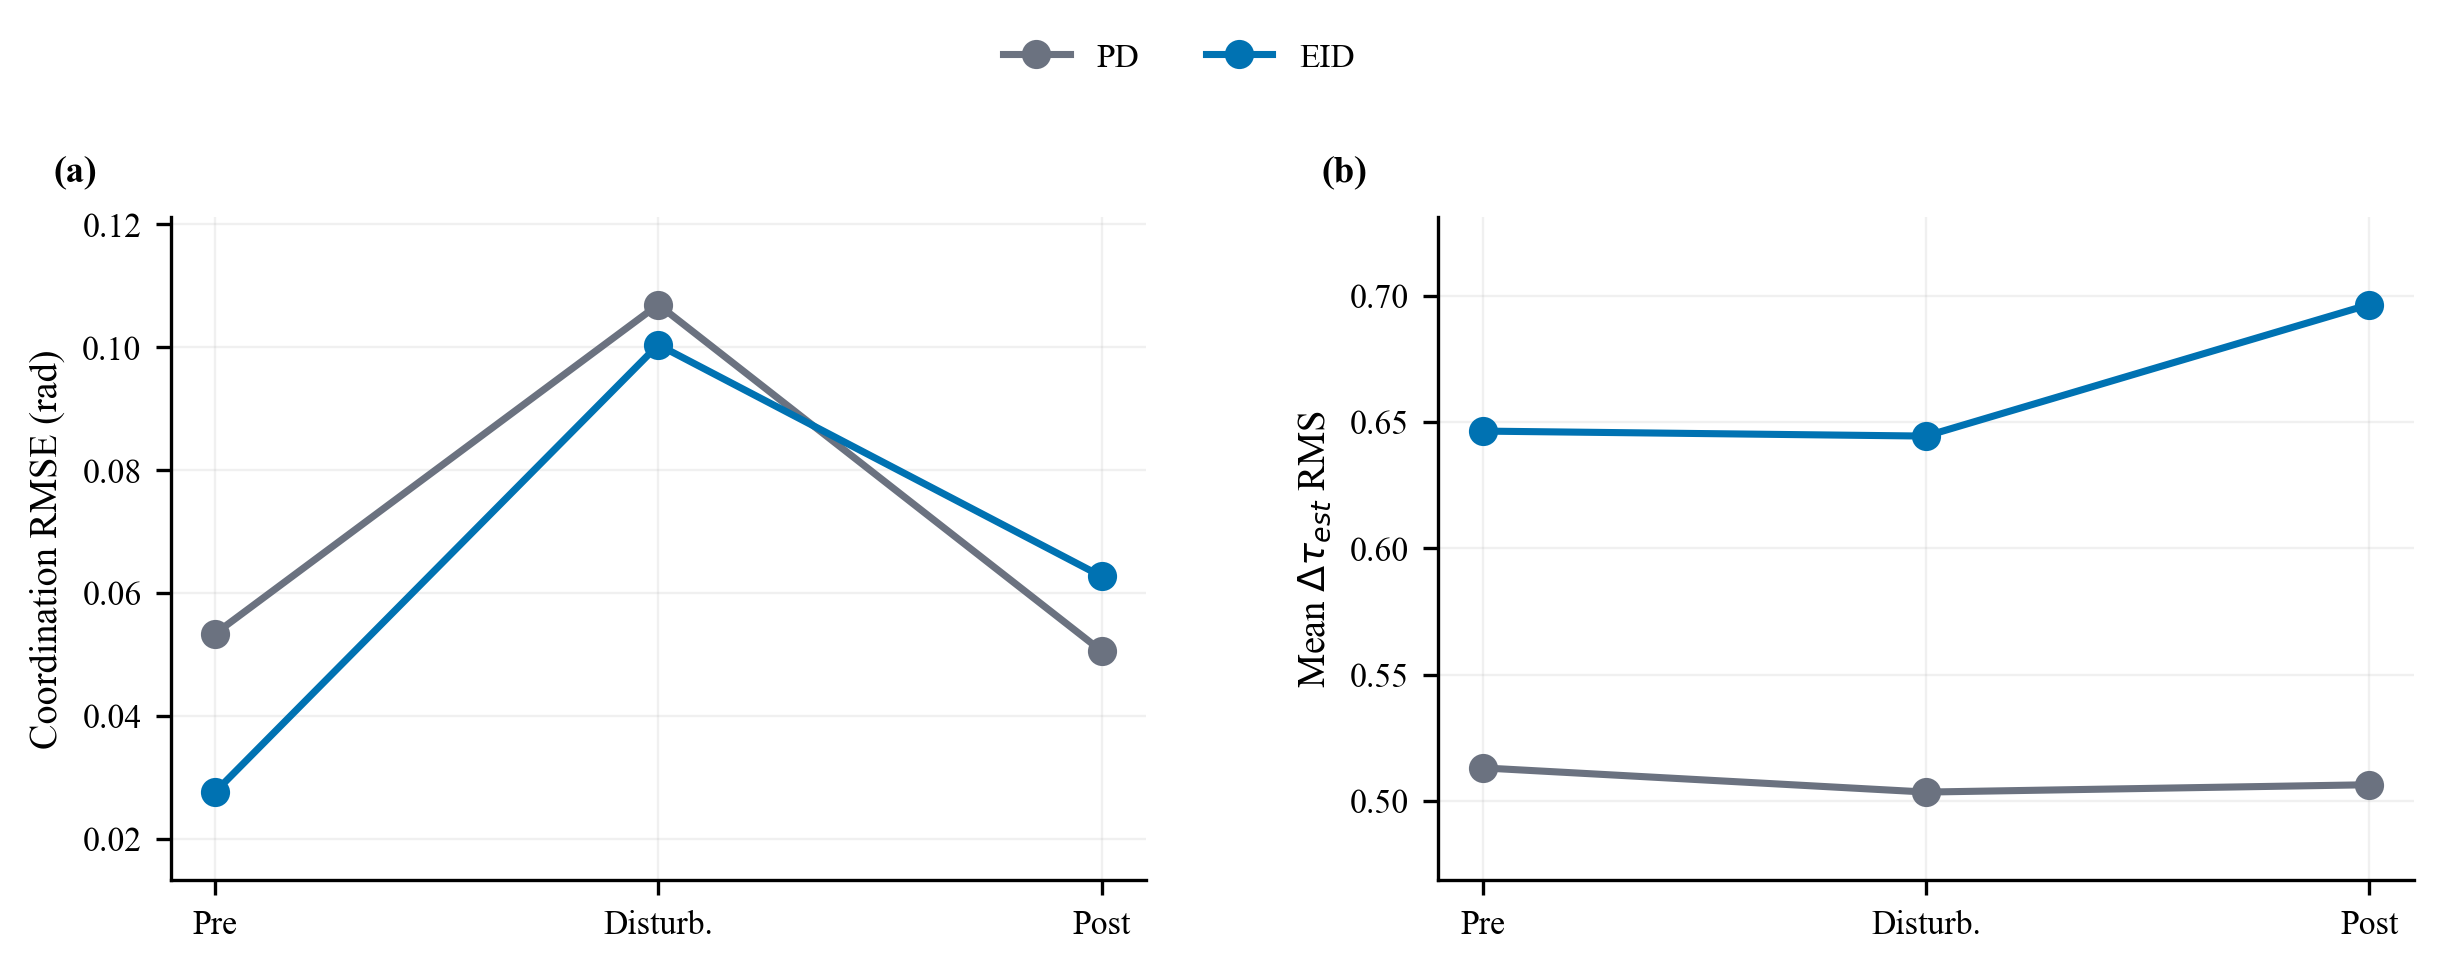
\includegraphics[keepaspectratio,alt={P2D 扰动窗口与恢复段统计}]{analysis_artifacts/bychen_answer/figures/bychen_p2d_window_recovery.png}}
\caption{P2D 扰动前、扰动窗口和恢复段统计。该图用于判断控制器是否只在扰动窗口内降低误差，却在扰动撤除后引入力矩活动或恢复段误差。恢复段仍属于软件输入端扰动实验，不能替代真实接触外扰实验。}
\end{figure}

\subsection{2.2 协调 RMSE 下降需要分解}

协调误差定义为

\[
e_{\rm coord}=e_{\rm hip}-e_{\rm knee}.
\]

因此协调 RMSE 的平方满足

\[
\mathrm{RMSE}_{\rm coord}^{2}
=E[(e_{\rm hip}-e_{\rm knee})^2]
=E[e_{\rm hip}^{2}]+E[e_{\rm knee}^{2}]-2E[e_{\rm hip}e_{\rm knee}].
\]

这意味着协调 RMSE 的下降可能来自髋误差下降、膝误差下降，或髋膝误差相关项变化。P2D 中膝 RMSE 上升而协调 RMSE 下降，所以必须把协调指标写成分解结果，而不能直接写成``双关节协调整体改善''。

\begin{longtable}[]{@{}lrrrr@{}}
\caption{P2D 协调误差均方分解。各项为 5 次完整扰动窗口重复的均值，单位为 rad\(^2\)。直接计算的 \(E[e_{\rm coord}^2]\) 与三项重构误差的最大绝对误差为 \(1.73\times 10^{-18}\)。}\\
\toprule
方法 & \(E[e_{\rm hip}^{2}]\) & \(E[e_{\rm knee}^{2}]\) & \(-2E[e_{\rm hip}e_{\rm knee}]\) & \(E[e_{\rm coord}^{2}]\) \\
\midrule
\endfirsthead
\toprule
方法 & \(E[e_{\rm hip}^{2}]\) & \(E[e_{\rm knee}^{2}]\) & \(-2E[e_{\rm hip}e_{\rm knee}]\) & \(E[e_{\rm coord}^{2}]\) \\
\midrule
\endhead
\bottomrule
\endlastfoot
PD & 0.003985 & 0.002047 & 0.005401 & 0.011433 \\
EID & 0.002666 & 0.002477 & 0.004934 & 0.010077 \\
\end{longtable}

\begin{figure}[H]
\centering
\pandocbounded{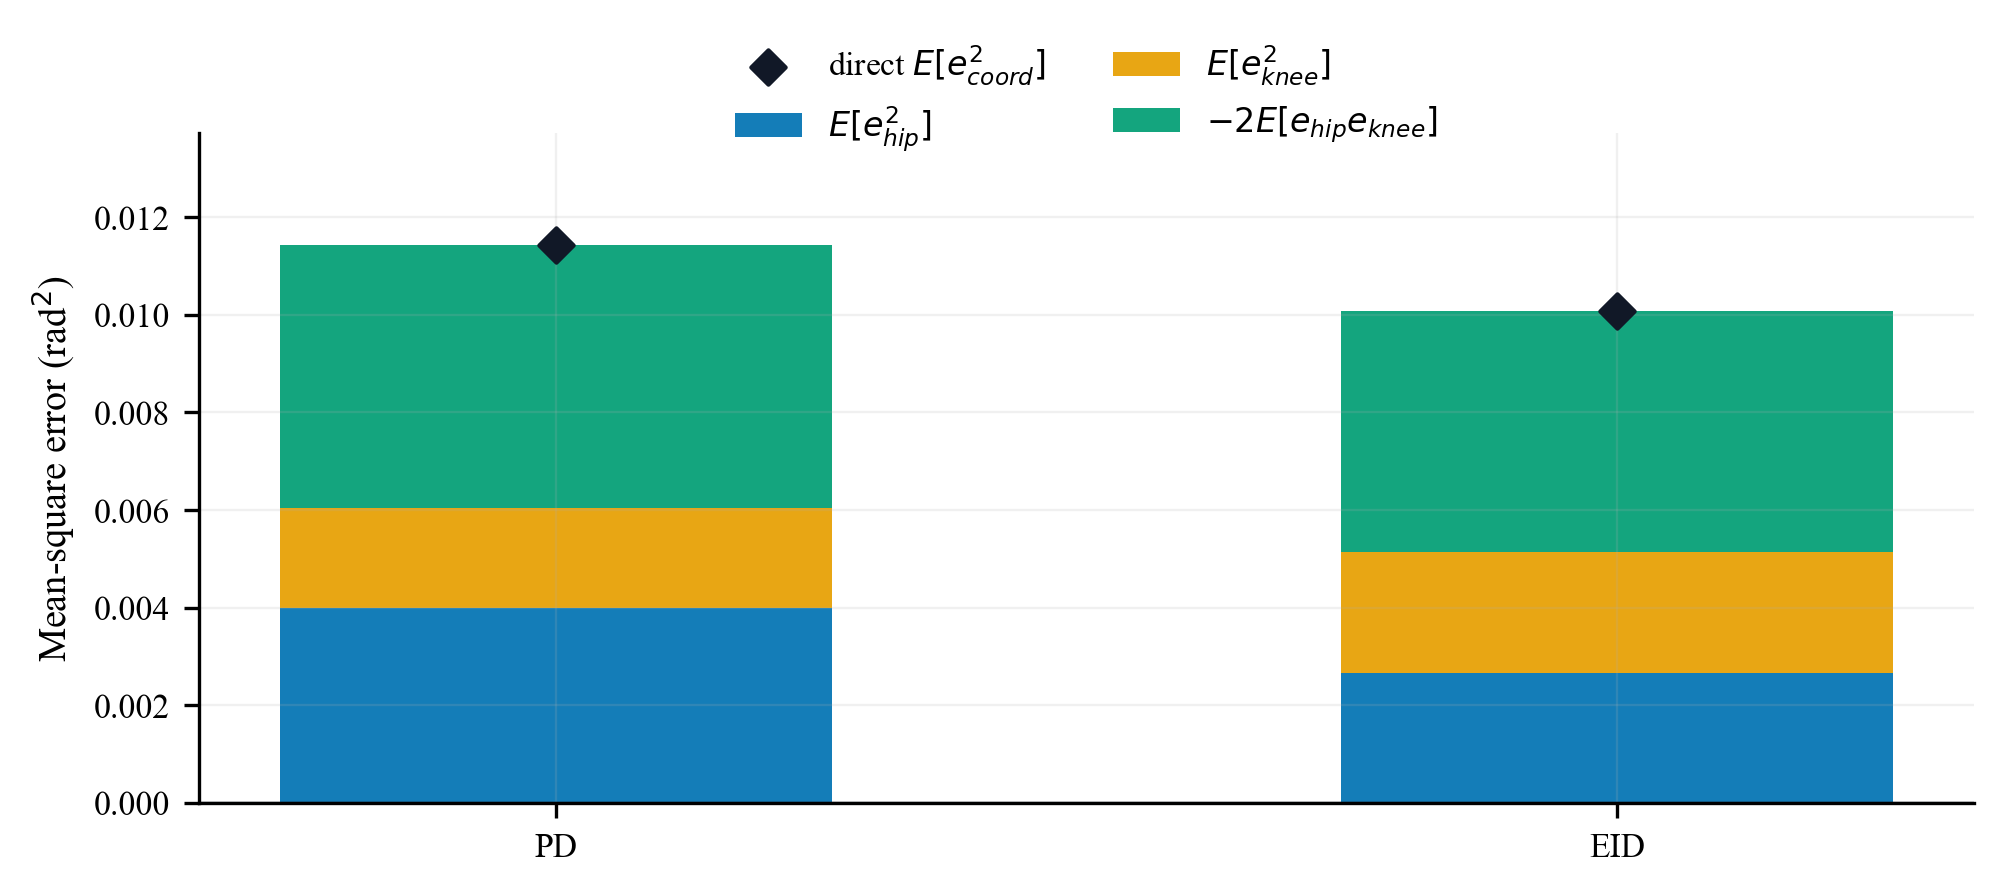
\includegraphics[keepaspectratio,alt={P2D 协调误差分解}]{analysis_artifacts/bychen_answer/figures/bychen_coord_decomposition.png}}
\caption{P2D 协调误差均方分解。EID 降低了髋误差项和相关项贡献，但膝误差项上升；因此协调 RMSE 的下降应解释为误差结构重分配，而不是髋膝两个关节同时变好。}
\end{figure}

\section{3. 机制证据：\texorpdfstring{\(\eta_u=K_u\eta\)}{eta_u=K_u eta} 不是当前主要 RMSE 杠杆}
\label{sec:mechanism}

如果 \(\eta_u=K_u\eta\) 是当前主要抗扰通道，那么它应在幅值、相位或结构消融中表现出对输入端残差的解释力。需要注意的是，当前日志能直接给出的只是软件力矩脉冲；对膝关节而言，完整输入端残差还包含第 2.1 节所述的非惯性项和髋膝耦合项。因此，本节的 \(\eta_u\) 对齐结果只能否定``\(\eta_u\) 直接等于软件脉冲估计''这一解释；它不能单独否定 \(\eta_u\) 对复合膝端残差的响应。尽管如此，P4D 的 \(K_u\) 扫描、力矩项分解和 MuJoCo 结构消融仍共同显示：当前窗口 RMSE 的主要变化更接近反馈中心与残差通道，而不是直接输入补偿项。

\subsection{3.1 当前 EID 更新带有对自身 \texorpdfstring{\(\eta\)}{eta} 的反馈}

控制算法说明中，EID 更新使用的是 \(x_k-\bar{x}_k\)，而不是 \(x_k-\hat{x}_k\)。由于

\[
\bar{x}_k=\hat{x}_k+\eta_k,
\]

残差实际为

\[
x_k-\bar{x}_k=x_k-\hat{x}_k-\eta_k.
\]

将该关系代入更新式，可写成

\[
\eta_{k+1}
=\alpha K_o(x_k-\hat{x}_k)
\left[(1-\alpha)I-\alpha K_o\right]\eta_k.
\]

因此，\(\eta\) 是带自反馈的残差滤波状态。这个结构解释了为什么继续放大 \(K_u\) 不一定降低 RMSE：如果 \(\eta\) 本身没有与输入端复合残差干净对齐，增大 \(K_u\) 更可能把内部活动注入力矩端。

\subsection{3.2 \texorpdfstring{\(\eta_u\)}{eta_u} 与软件脉冲不对齐}

下表使用的是 \(\eta_u\) 与日志中已知软件脉冲 \(\tau_d\) 的对齐，而不是与第 2.1 节定义的膝端复合输入残差 \(d_{k,\rm in}\) 的对齐。因此，它适合回答一个较窄的问题：当前 \(\eta_u\) 是否可以被解释成软件脉冲的直接估计。它不适合回答更强的问题：\(\eta_u\) 是否已经吸收了髋段加速度折合到膝端的非惯性扰动。

\begin{longtable}[]{@{}llrrr@{}}
\caption{\(\eta_u\) 与已知软件脉冲的对齐摘要。RMS 比值为 \(\mathrm{RMS}(\eta_u)/\mathrm{RMS}(\tau_d)\)，相关性使用 \(-\eta_u\) 与 \(\tau_d\) 比较；\(\tau_d\) 不包含膝端非惯性耦合残差。}\\
\toprule
组别 & 关节 & RMS 比值 & 零滞后相关 & 最优相关 \\
\midrule
\endfirsthead
\toprule
组别 & 关节 & RMS 比值 & 零滞后相关 & 最优相关 \\
\midrule
\endhead
\bottomrule
\endlastfoot
P2D & Hip & 0.00394 & -0.312 & -0.319 \\
P2D & Knee & 0.01296 & -0.610 & -0.623 \\
O5 & Hip & 0.00540 & -0.182 & -0.196 \\
O5 & Knee & 0.01298 & -0.623 & -0.635 \\
U1 & Hip & 0.00196 & -0.296 & -0.308 \\
U1 & Knee & 0.00656 & -0.631 & -0.643 \\
\end{longtable}

\begin{figure}[H]
\centering
\pandocbounded{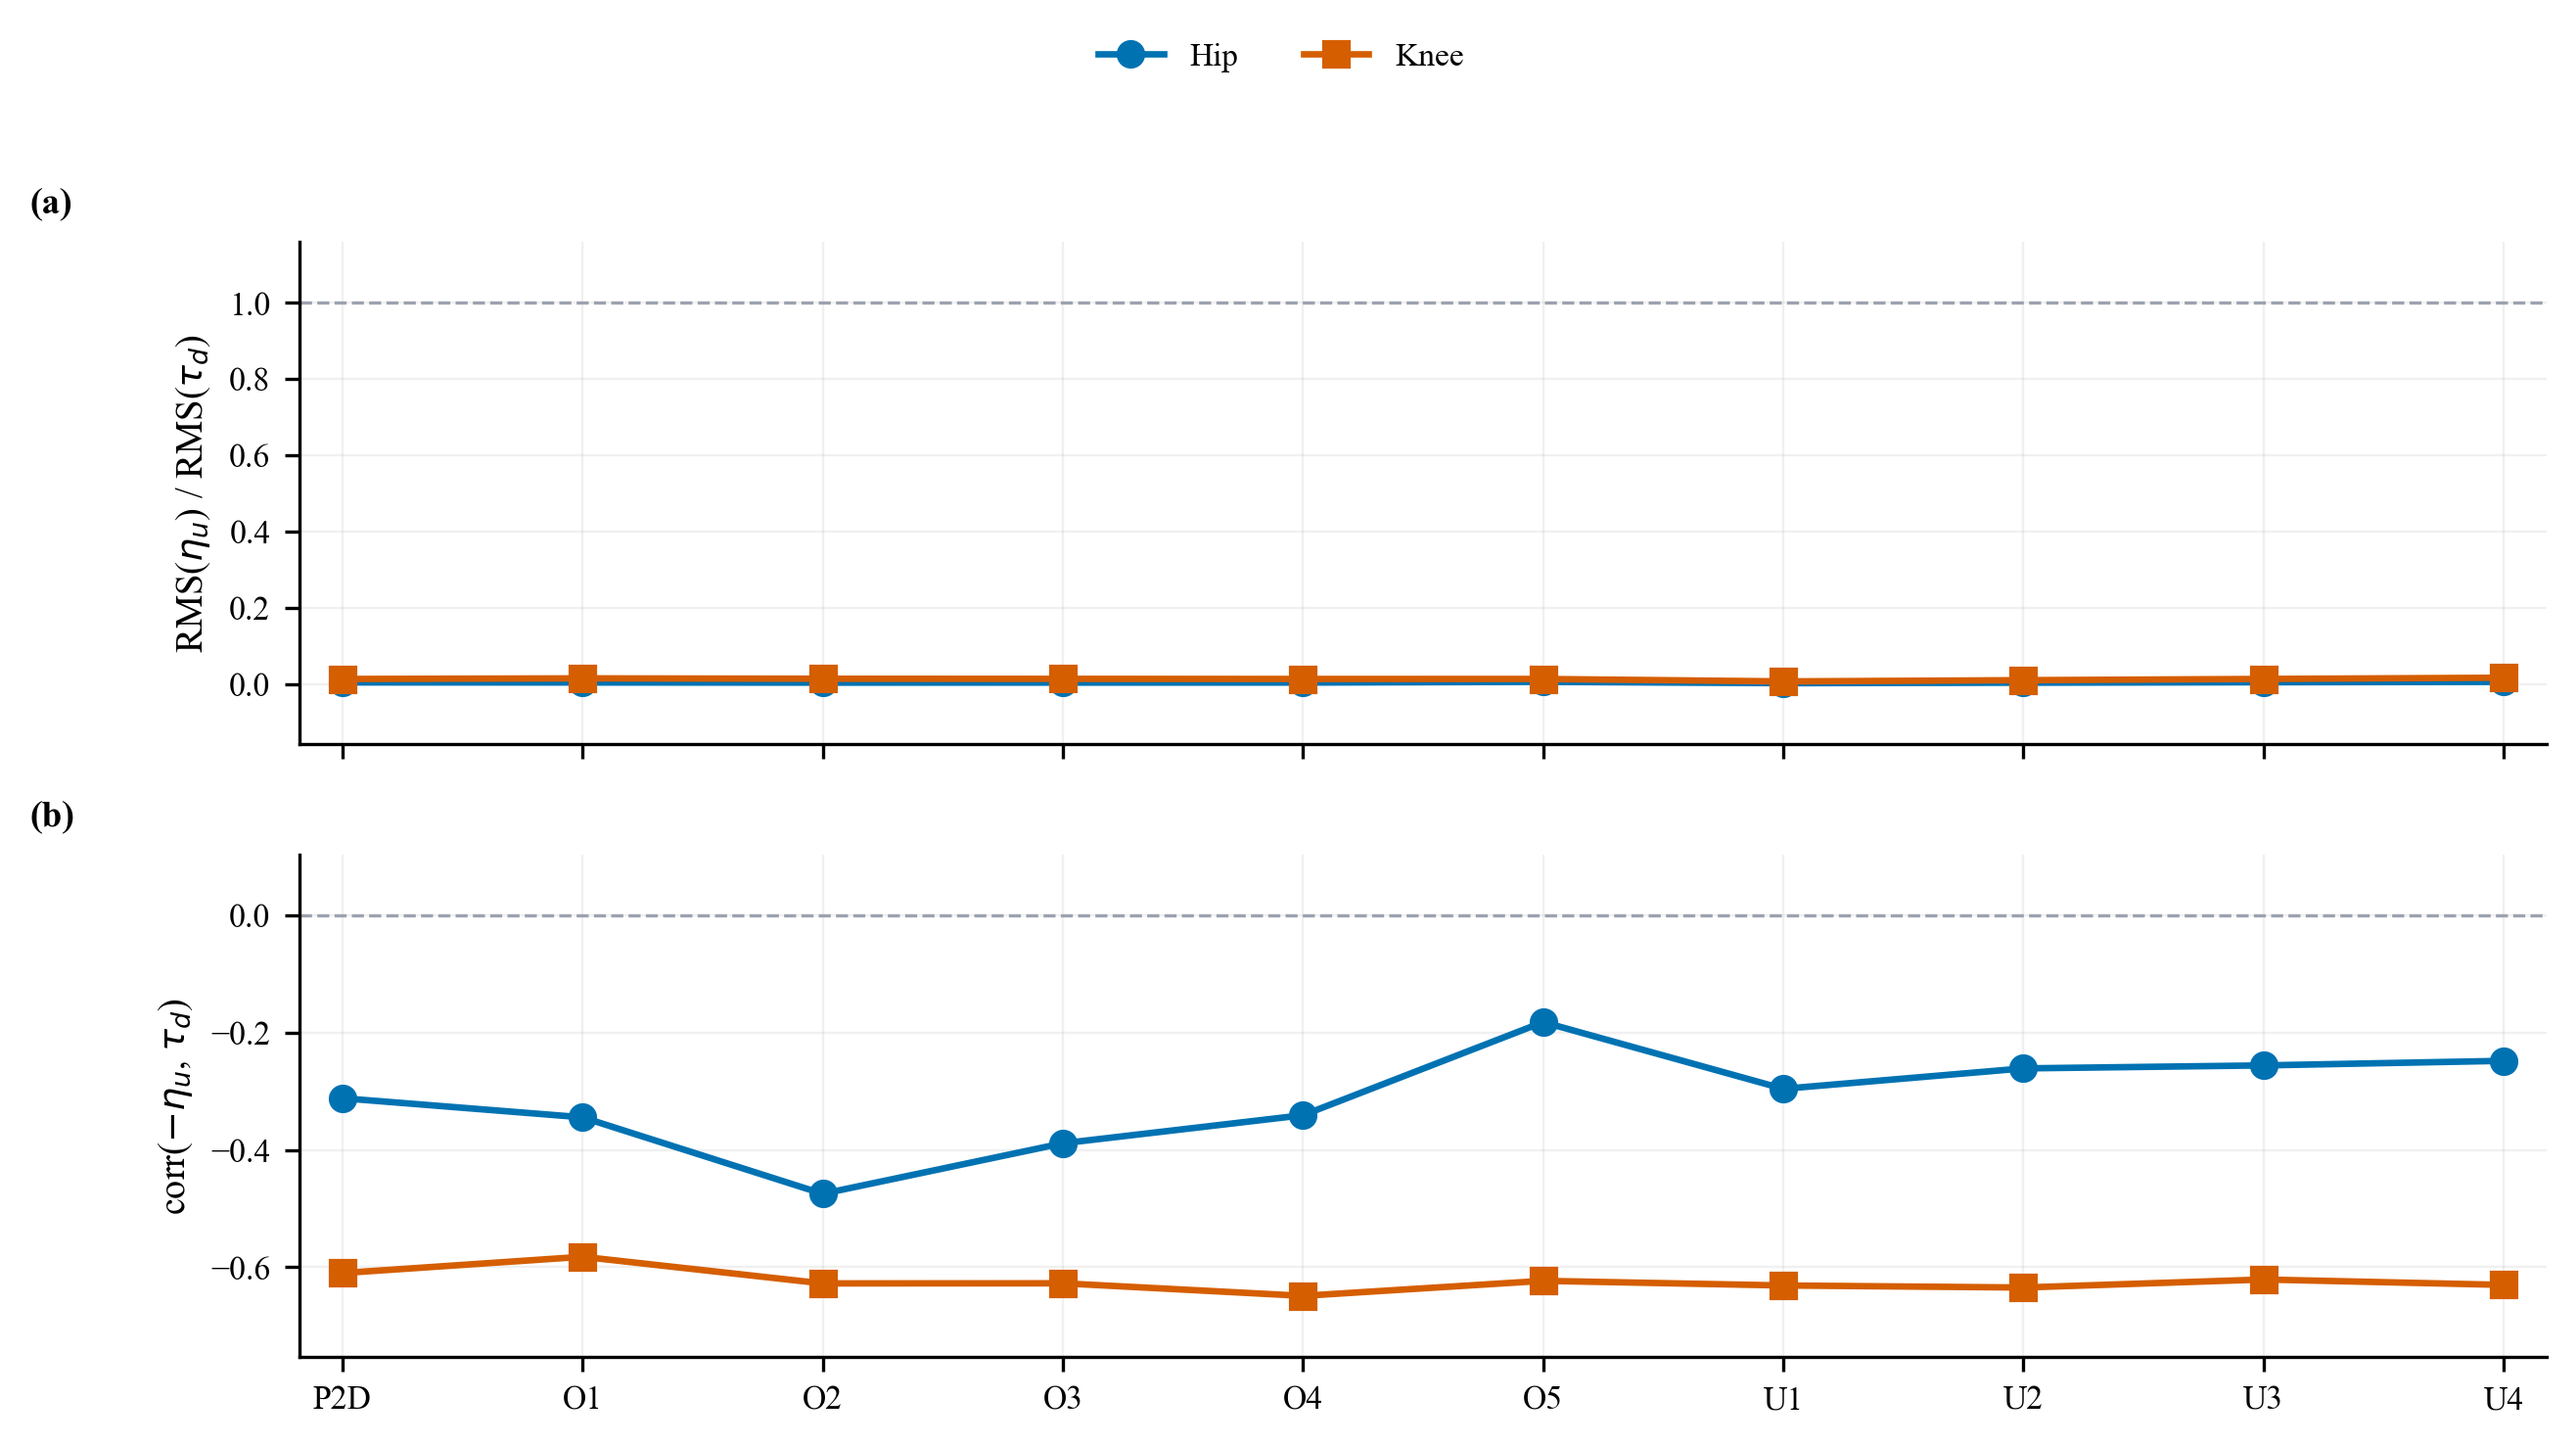
\includegraphics[keepaspectratio,alt={eta_u 与软件扰动对齐}]{analysis_artifacts/bychen_answer/figures/bychen_eta_disturbance_alignment.png}}
\caption{\(\eta_u\) 与软件输入端力矩脉冲对齐。当前 \(\eta_u\) 的幅值远小于已知软件脉冲，相关性也不支持将其直接解释为软件脉冲估计；膝端复合输入残差仍需另行由动力学模型重构。}
\end{figure}

\subsection{3.3 力矩项分解显示反馈项远大于输入补偿项}

\begin{longtable}[]{@{}llrrrr@{}}
\caption{扰动窗口内 EID 力矩项 RMS 分解，单位为 N m。}\\
\toprule
组别 & 关节 & \(u^\star\) & \(u_{\rm fb}\) & \(-\eta_u\) & \(u_t\) \\
\midrule
\endfirsthead
\toprule
组别 & 关节 & \(u^\star\) & \(u_{\rm fb}\) & \(-\eta_u\) & \(u_t\) \\
\midrule
\endhead
\bottomrule
\endlastfoot
P2D & Hip & 2.581 & 6.001 & 0.0214 & 7.845 \\
P2D & Knee & 1.124 & 5.327 & 0.0470 & 5.543 \\
O5 & Hip & 2.579 & 5.830 & 0.0294 & 7.662 \\
O5 & Knee & 1.124 & 5.301 & 0.0471 & 5.627 \\
U1 & Hip & 2.580 & 5.811 & 0.0107 & 7.665 \\
U1 & Knee & 1.124 & 5.242 & 0.0238 & 5.602 \\
\end{longtable}

\begin{figure}[H]
\centering
\pandocbounded{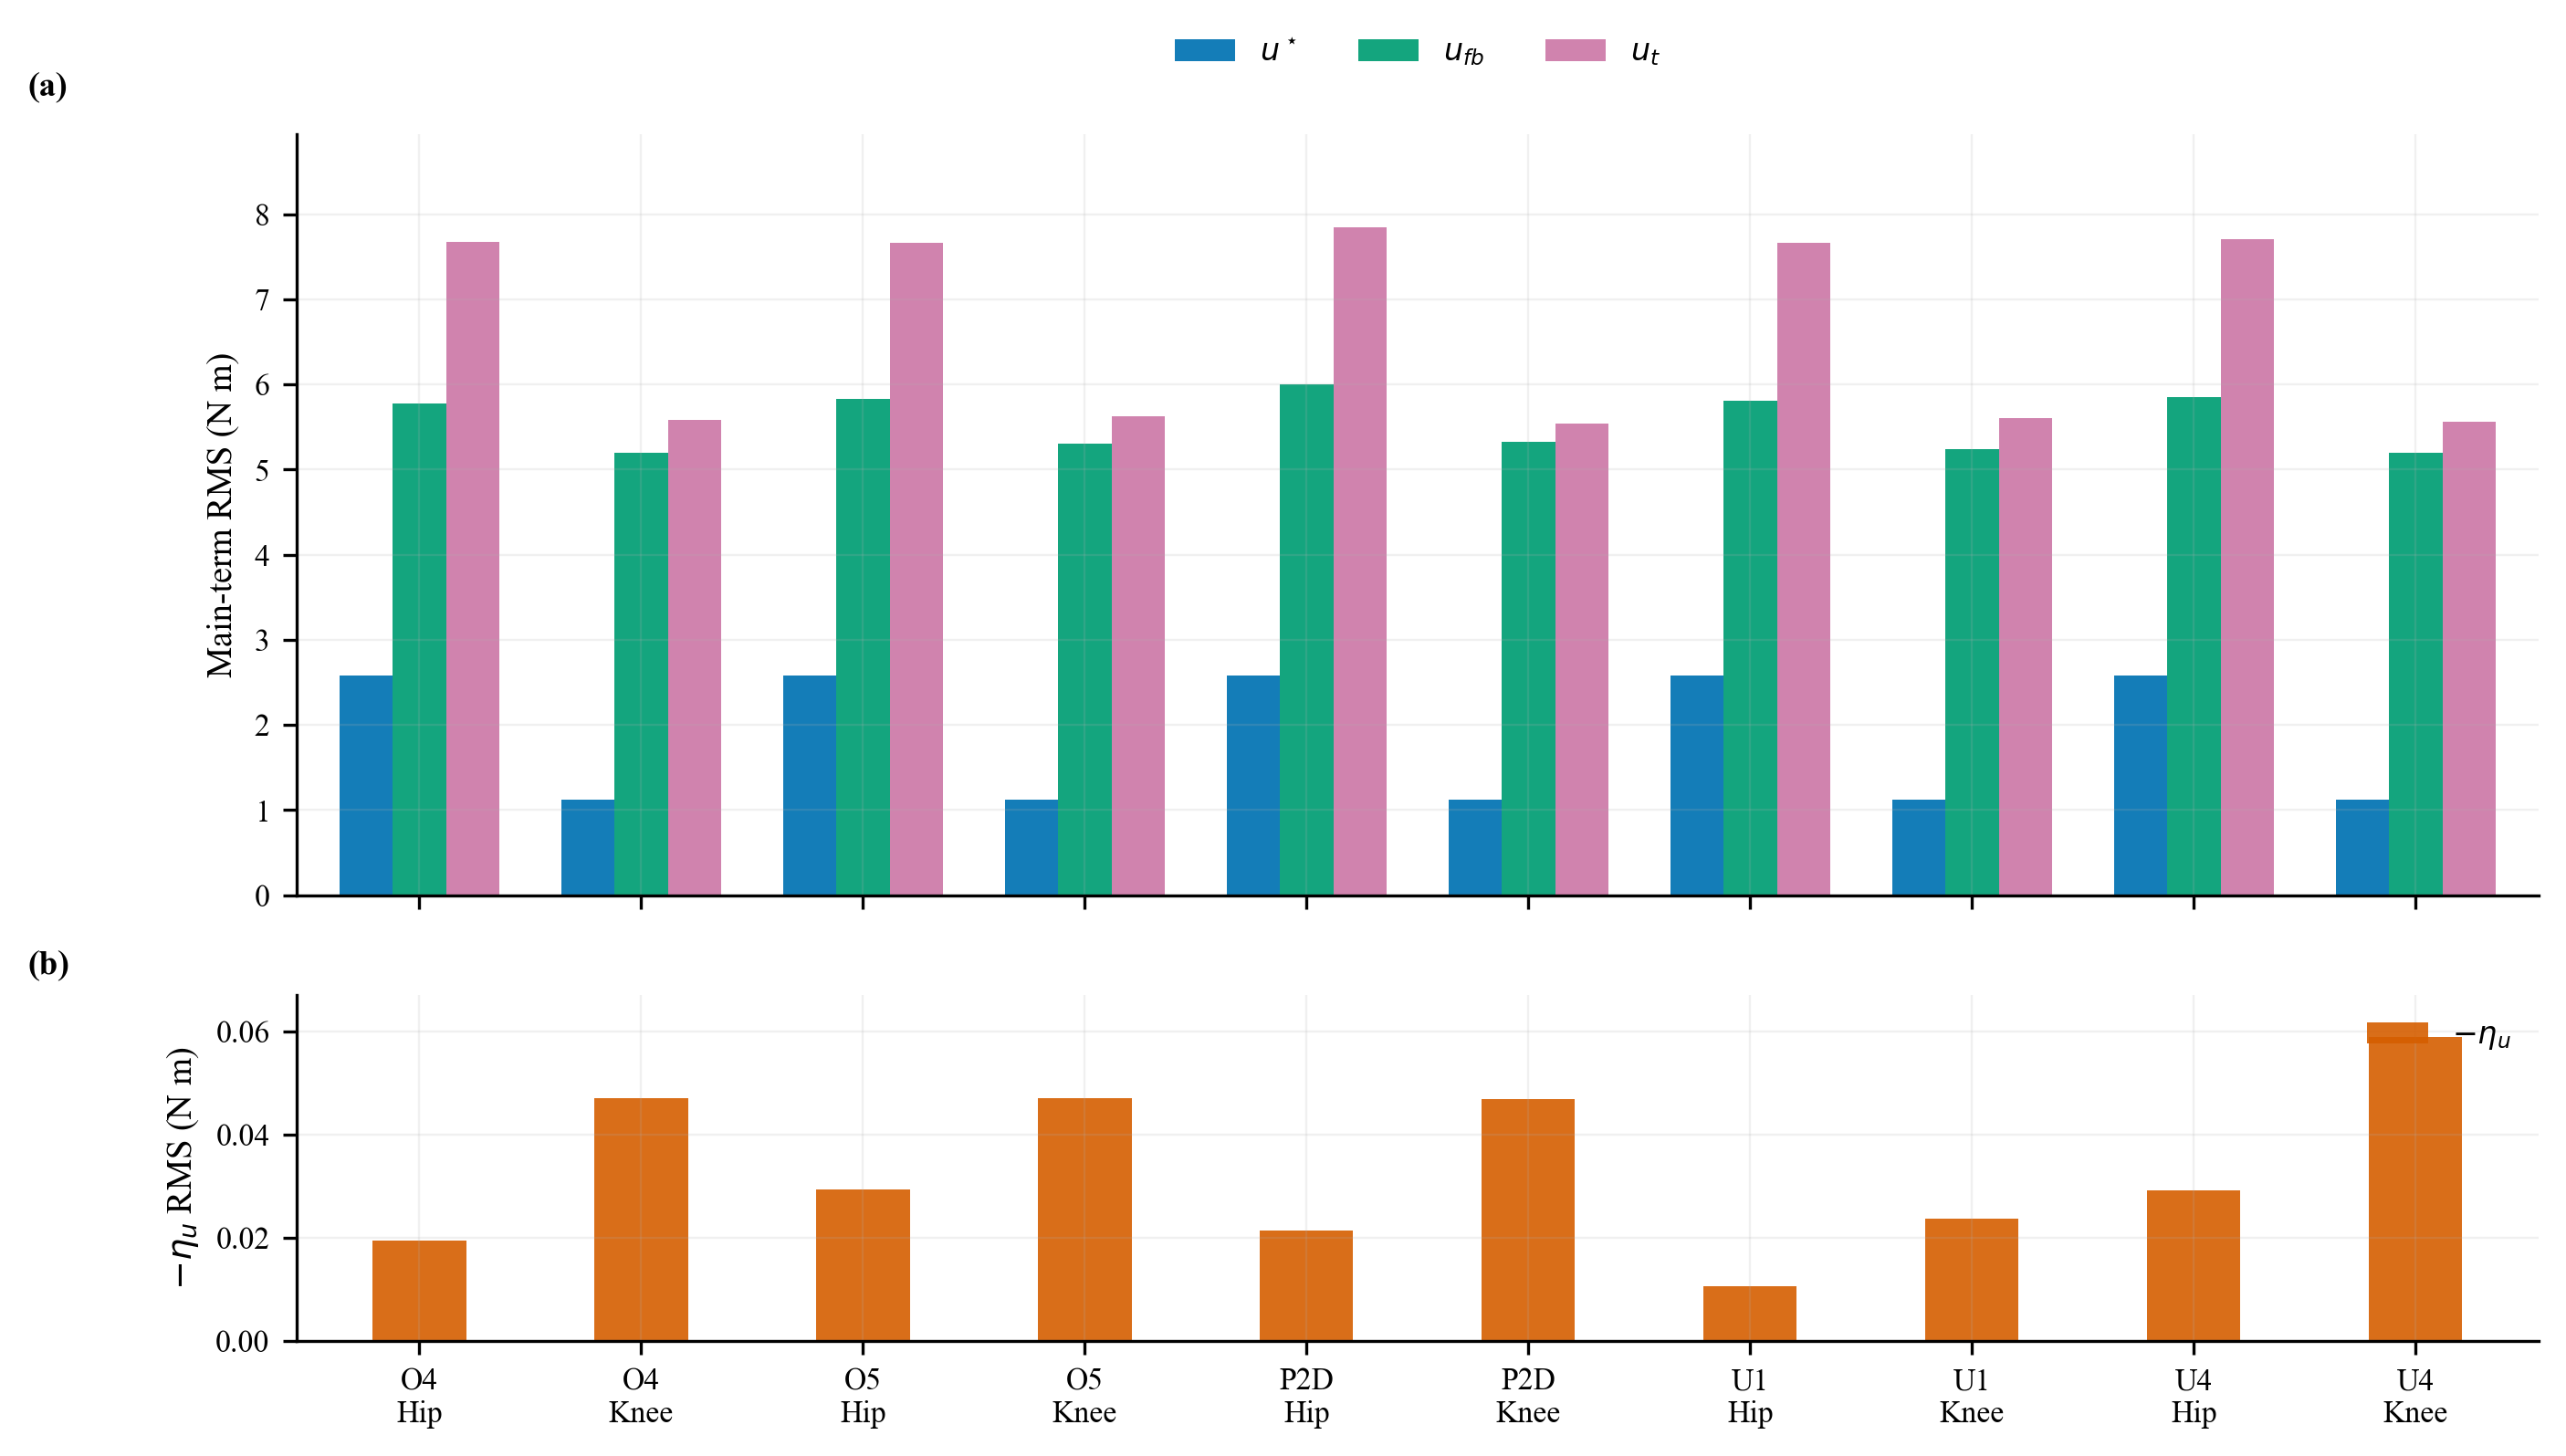
\includegraphics[keepaspectratio,alt={力矩项分解}]{analysis_artifacts/bychen_answer/figures/bychen_force_decomposition.png}}
\caption{扰动窗口内力矩项分解。反馈项 RMS 远大于 \(-\eta_u\) 输入补偿项，支持将当前主要可调性放在反馈中心、残差定义和 \(K_o\) 通道上，而不是直接放在 \(\eta_u=K_u\eta\) 上。}
\end{figure}

\subsection{3.4 结构消融与残差扫描的指向}

结构消融的目的，是把完整 EID 拆成几种可理解的功能块，判断误差收益更像来自哪一块。这里比较四种模式：只保留解析逆模型、只保留输入补偿 \(-\eta_u\)、只改变反馈中心 \(\bar{x}\)、以及完整 EID。结果显示，在 \(\mathrm{O4+U1}\) 与 \(\mathrm{O5+U1}\) 两个候选上，“只保留输入补偿”与“只保留解析逆模型”的协调 RMSE 非常接近，而“只改变反馈中心”与“完整 EID”更接近。因此，当前收益更像来自反馈中心和残差通道，而不是直接来自 \(-\eta_u\) 输入补偿。

\begin{longtable}[]{@{}llrrr@{}}
\caption{MuJoCo 结构消融摘要。该表只用于机理解释，不用于给出实机安全结论。}\\
\toprule
候选 & 消融模式 & 协调 RMSE & 膝 \(\Delta\tau_{\rm total}\) RMS & 膝 \(\eta_u\) RMS \\
\midrule
\endfirsthead
\toprule
候选 & 消融模式 & 协调 RMSE & 膝 \(\Delta\tau_{\rm total}\) RMS & 膝 \(\eta_u\) RMS \\
\midrule
\endhead
\bottomrule
\endlastfoot
\(\mathrm{O4+U1}\) & 只保留解析逆模型 & 0.059987 & 0.132226 & 0.000000 \\
\(\mathrm{O4+U1}\) & 只保留输入补偿 & 0.059821 & 0.132180 & 0.015753 \\
\(\mathrm{O4+U1}\) & 只改变反馈中心 & 0.067726 & 0.137277 & 0.000000 \\
\(\mathrm{O4+U1}\) & 完整 EID & 0.067562 & 0.137295 & 0.015854 \\
\(\mathrm{O5+U1}\) & 只保留解析逆模型 & 0.059987 & 0.132226 & 0.000000 \\
\(\mathrm{O5+U1}\) & 只保留输入补偿 & 0.059822 & 0.132128 & 0.015572 \\
\(\mathrm{O5+U1}\) & 只改变反馈中心 & 0.066155 & 0.138418 & 0.000000 \\
\(\mathrm{O5+U1}\) & 完整 EID & 0.065995 & 0.138420 & 0.015655 \\
\end{longtable}

\begin{figure}[H]
\centering
\pandocbounded{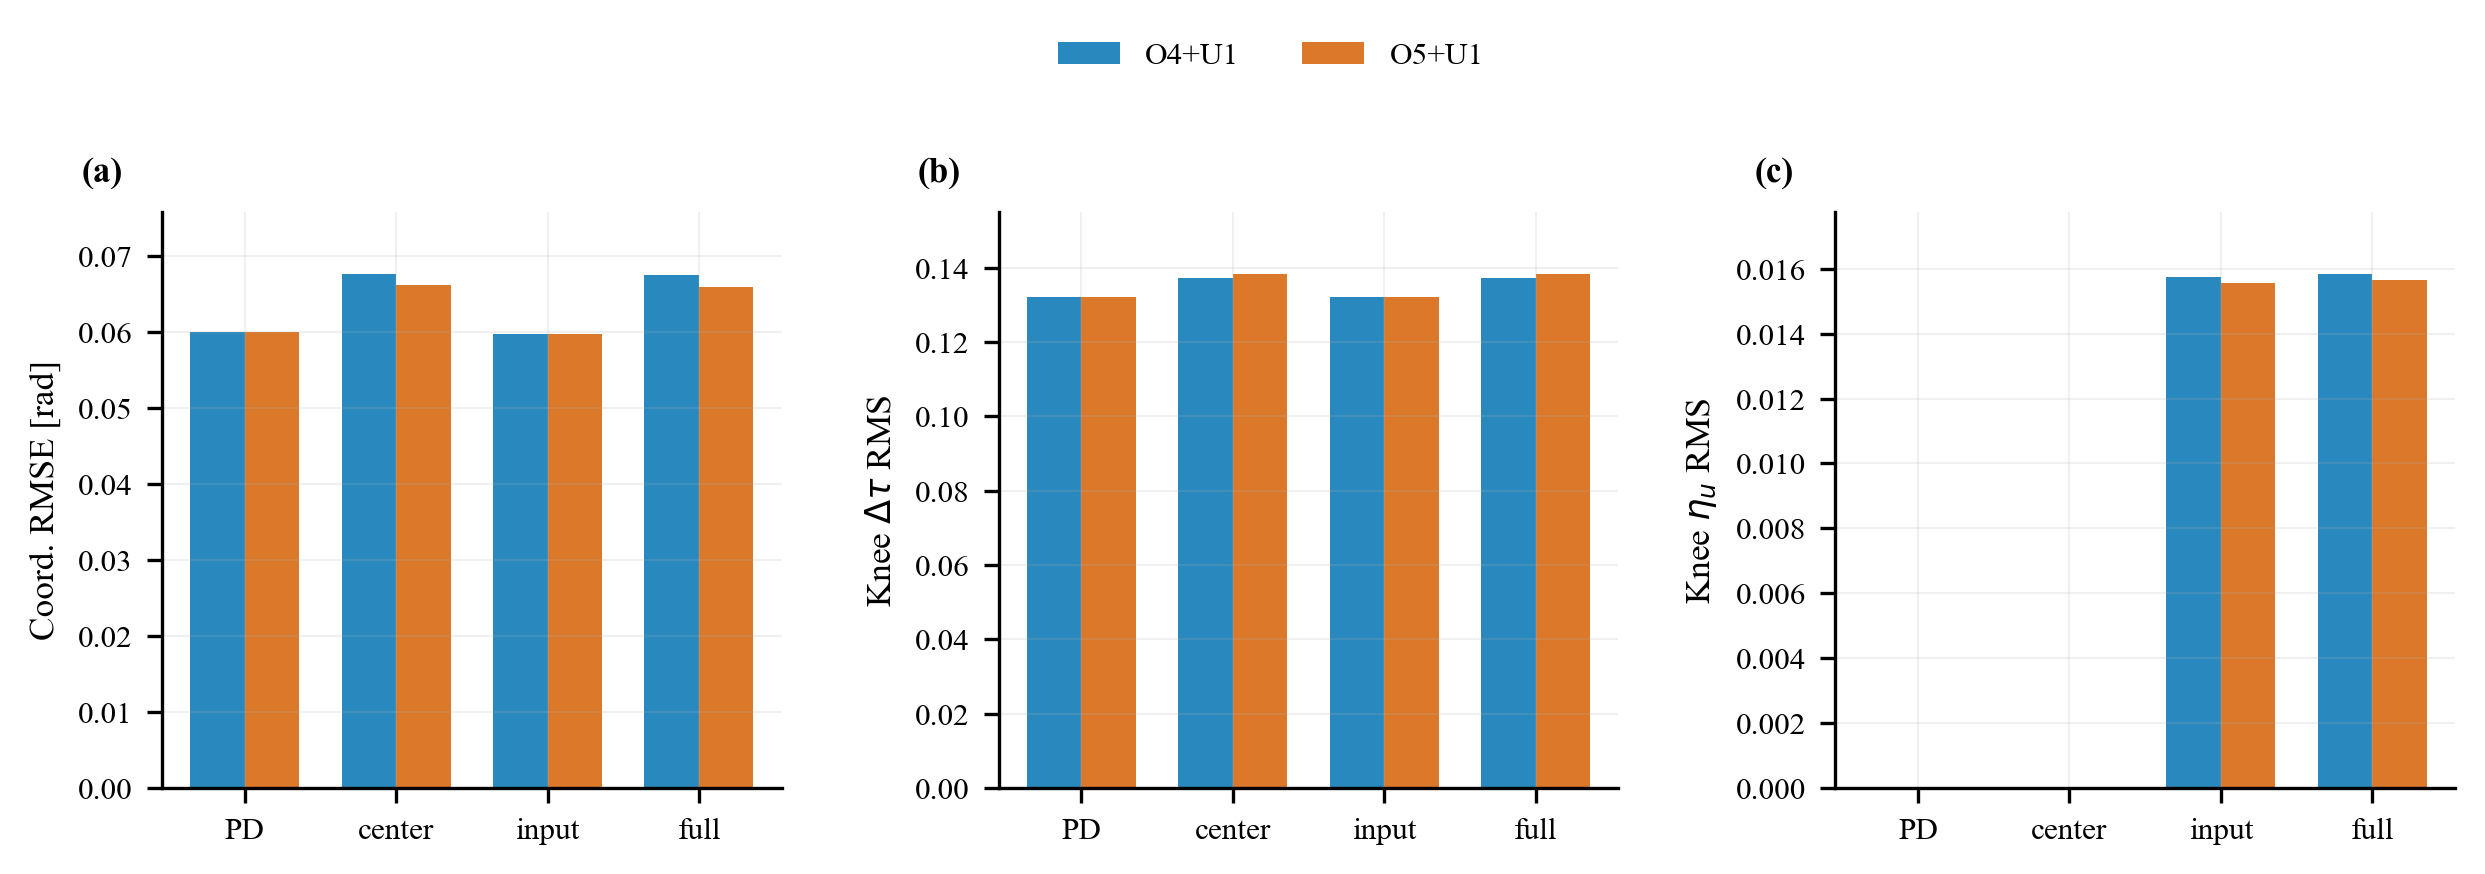
\includegraphics[keepaspectratio,alt={MuJoCo 结构消融}]{analysis_artifacts/bychen_mujoco_mechanism_completion/figures/mujoco_mechanism_structure_ablation.png}}
\caption{MuJoCo 结构消融。该结果支持将 \(\bar{x}\) 反馈中心和残差定义作为下一轮机理问题，而不是继续扩大 \(K_u\) 扫描。}
\end{figure}

残差 \(\lambda\) 扫描进一步说明，残差定义本身也是误差-力矩权衡。以 \(\mathrm{O5+U1}\) 为例，\(\lambda=0\) 将协调 RMSE 从 0.065995 降到 0.064238，但膝 \(\Delta\tau_{\rm total}\) RMS 从 0.138420 增到 0.139901。该趋势不支持把残差定义写成``越激进越好''，而应作为需要噪声和限幅约束进一步筛查的结构变量。

\begin{figure}[H]
\centering
\pandocbounded{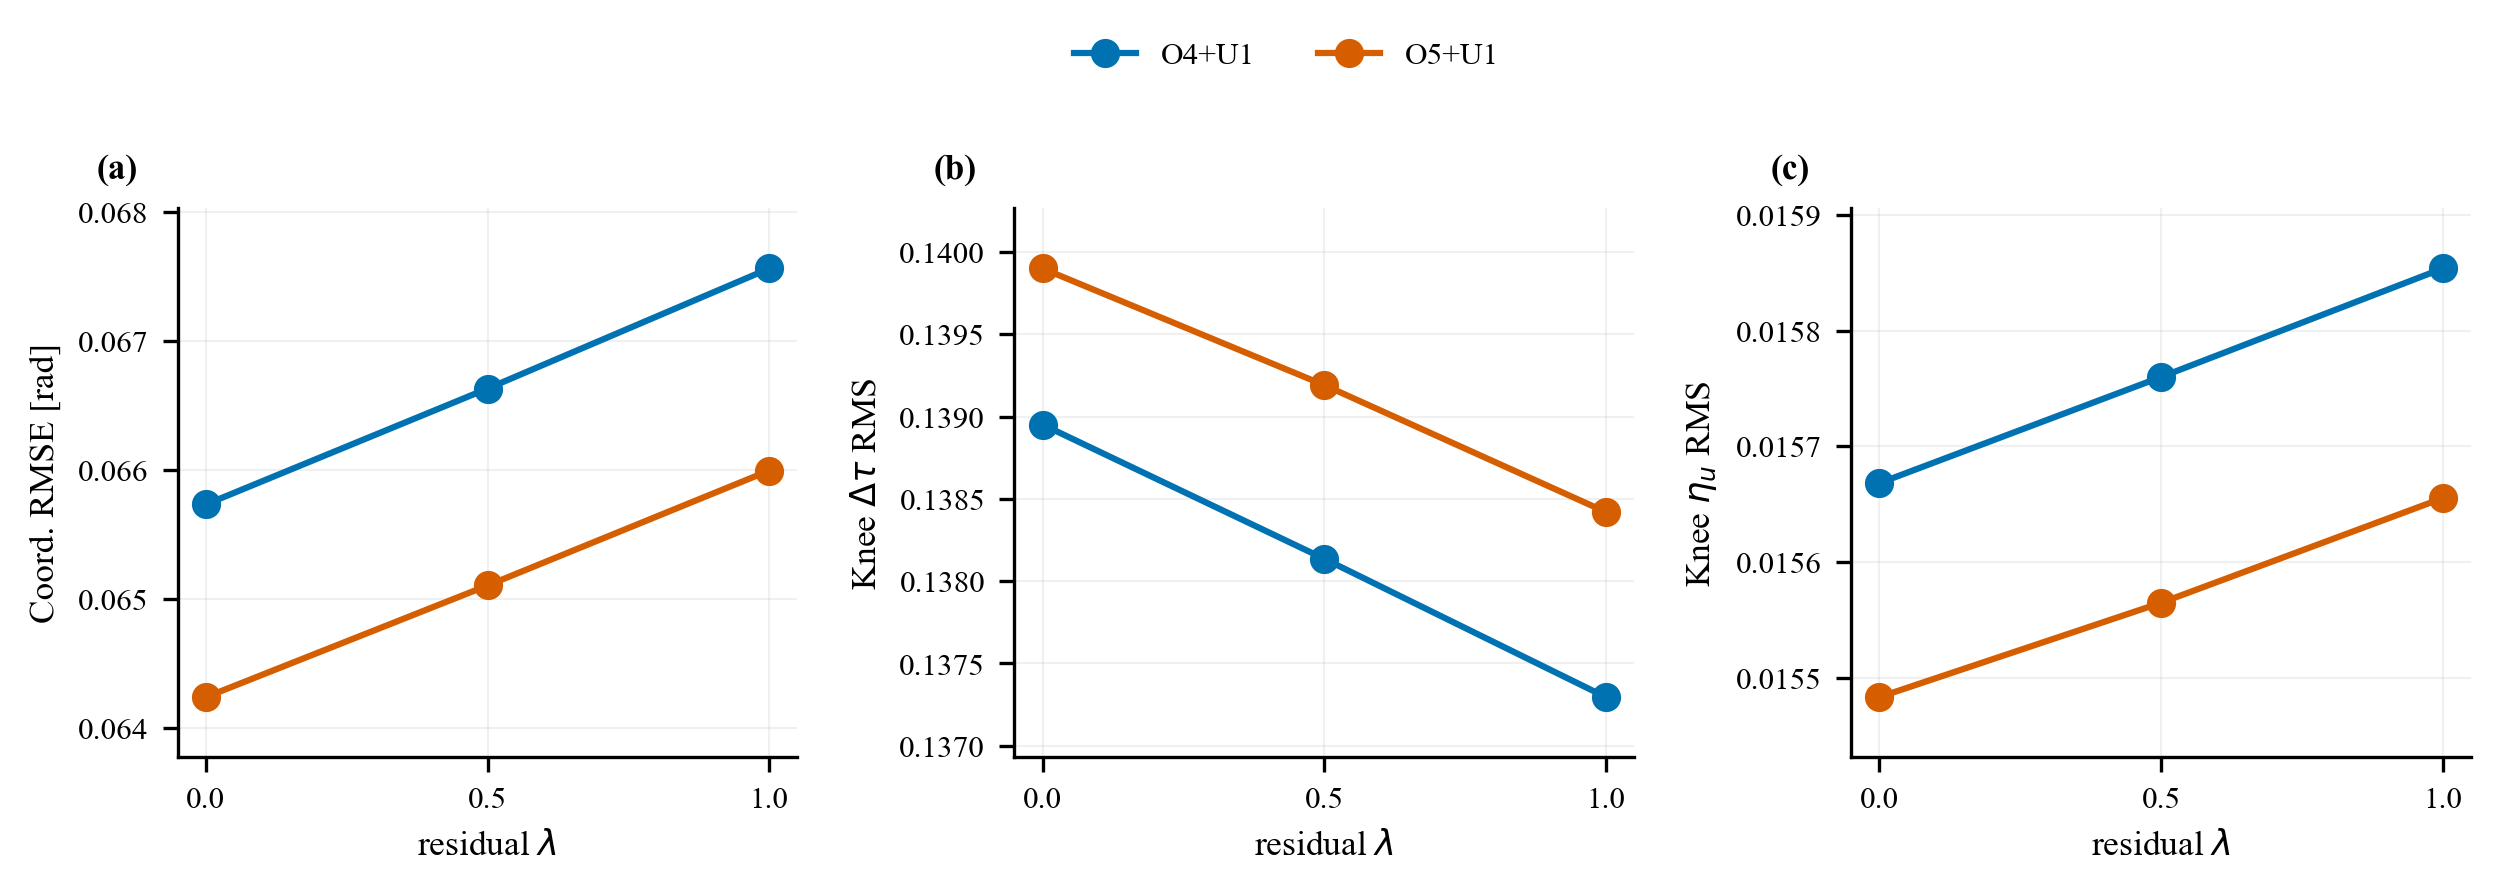
\includegraphics[keepaspectratio,alt={MuJoCo 残差 lambda 扫描}]{analysis_artifacts/bychen_mujoco_mechanism_completion/figures/mujoco_mechanism_residual_lambda.png}}
\caption{MuJoCo 残差 \(\lambda\) 扫描。较小 \(\lambda\) 与较低协调 RMSE 相关，但同时提高膝力矩变化量；该结果只支持机理筛查，不支持直接上机。}
\end{figure}

\section{4. 参数证据：\texorpdfstring{\(K_o\)}{K_o} 是性能杠杆，\texorpdfstring{\(K_u\)}{K_u} 是代价旋钮}
\label{sec:params}

P4D 参数扫描回答两个不同问题：共同提高 \(K_o\) 是否影响扰动窗口误差；提高 \(K_u\) 是否带来可辨识 RMSE 收益。当前结果显示，前者成立，后者不明显。

\subsection{4.1 共同 \texorpdfstring{\(K_o\)}{K_o} 扫描}

\begin{longtable}[]{@{}lrrrrrrrr@{}}
\caption{P4D 共同 \(K_o\) 扫描。\(\mathrm{O0}\) 未覆盖完整扰动窗口，因此不用于窗口 RMSE 排名。}\\
\toprule
组别 & \(s_o\) & 完整运行 & 完整窗口 & 髋 RMSE & 膝 RMSE & 协调 RMSE & 髋 \(\tau_{\rm est}\) RMS & 膝 \(\tau_{\rm est}\) RMS \\
\midrule
\endfirsthead
\toprule
组别 & \(s_o\) & 完整运行 & 完整窗口 & 髋 RMSE & 膝 RMSE & 协调 RMSE & 髋 \(\tau_{\rm est}\) RMS & 膝 \(\tau_{\rm est}\) RMS \\
\midrule
\endhead
\bottomrule
\endlastfoot
O0 & 0.00 & 0/3 & 0/3 & - & - & - & - & - \\
O1 & 0.25 & 2/3 & 3/3 & 0.0588 & 0.0755 & 0.1334 & 2.6362 & 2.5498 \\
O2 & 0.50 & 2/3 & 3/3 & 0.0529 & 0.0582 & 0.1101 & 2.5895 & 2.7183 \\
O3 & 0.75 & 2/3 & 3/3 & 0.0510 & 0.0532 & 0.1031 & 2.6378 & 2.9040 \\
O4 & 1.00 & 3/3 & 3/3 & 0.0499 & 0.0497 & 0.0984 & 2.6002 & 2.8164 \\
O5 & 1.25 & 3/3 & 3/3 & 0.0494 & 0.0485 & 0.0965 & 2.6647 & 2.8815 \\
\end{longtable}

\begin{figure}[H]
\centering
\pandocbounded{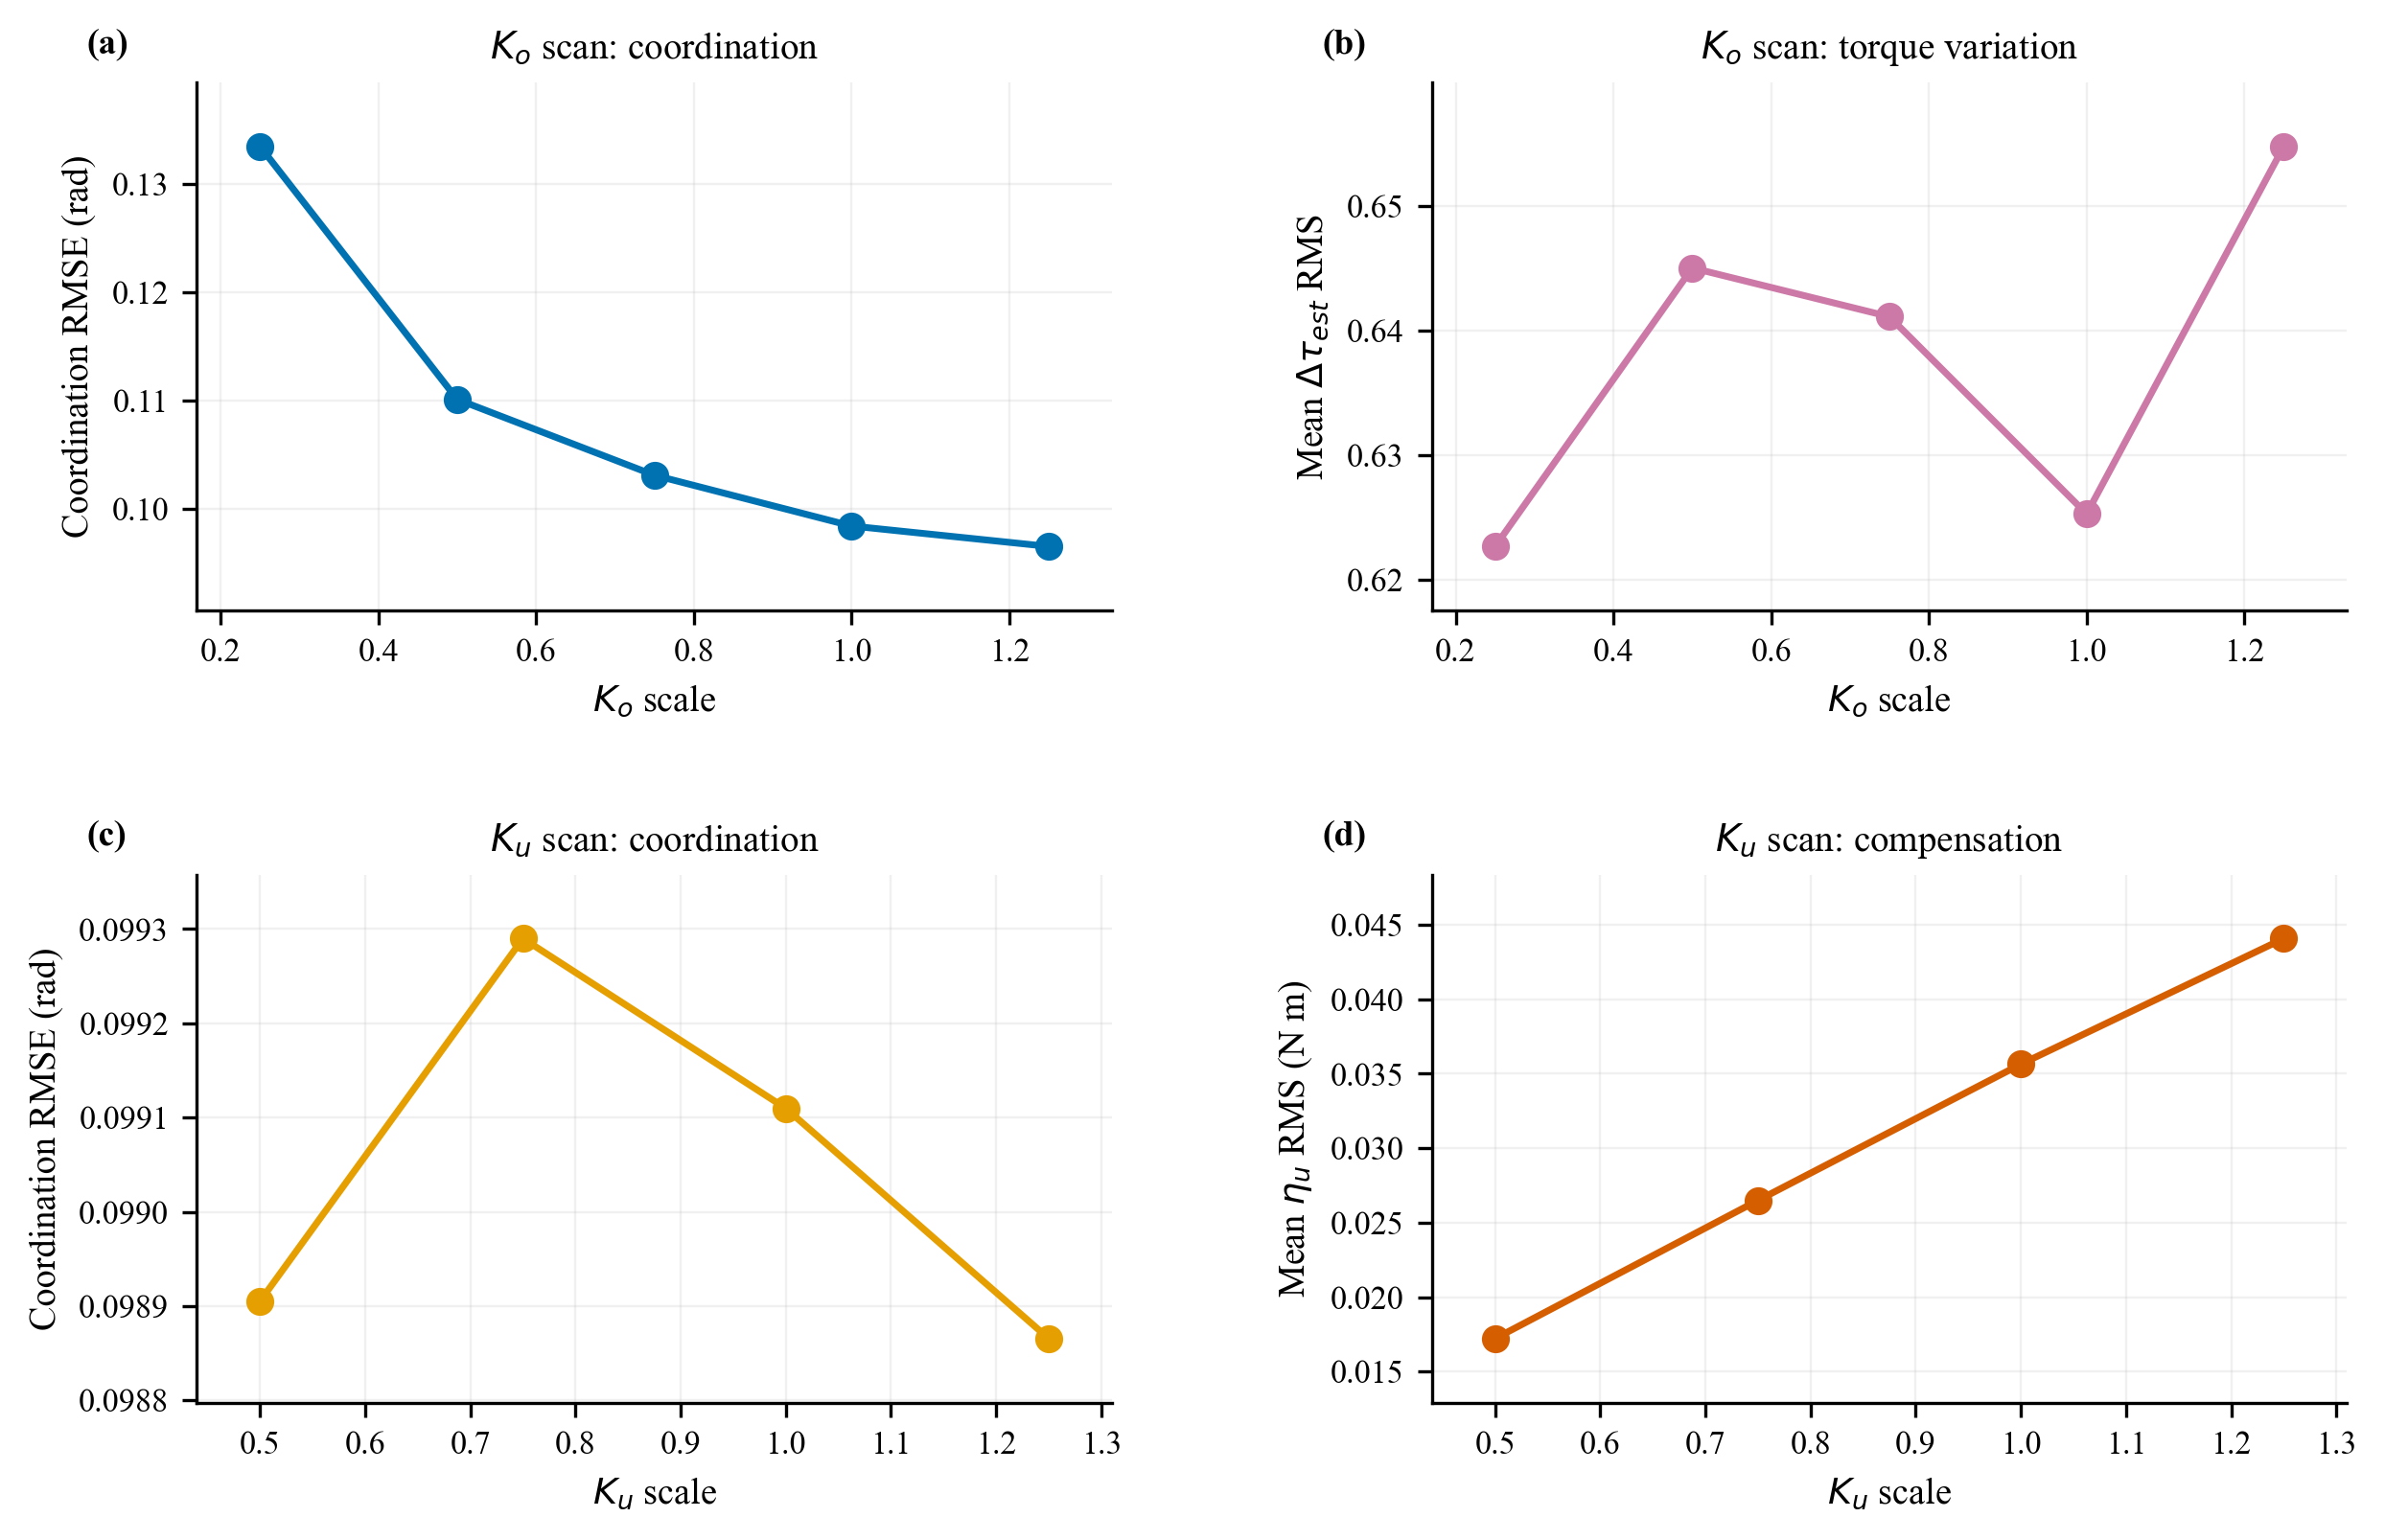
\includegraphics[keepaspectratio,alt={P4D 增益扫描}]{analysis_artifacts/bychen_answer/figures/bychen_p4d_gain_scans.png}}
\caption{P4D 增益扫描。共同 \(K_o\) 增大时窗口 RMSE 下降；\(K_u\) 扫描中窗口 RMSE 近似重合，但 \(\eta_u\) RMS 随倍率增大。}
\end{figure}

该结果只能说明共同提高髋膝 \(K_o\) 时窗口 RMSE 下降。它不回答哪个关节、哪个通道应该提高或降低。因此，下一轮不应继续做 \(\mathrm{O6}\)/\(\mathrm{O7}\) 这类一维共同倍率扫描，而应做逐关节机制矩阵。

\subsection{4.2 \texorpdfstring{\(K_u\)}{K_u} 扫描}

\begin{longtable}[]{@{}lrrrrrrr@{}}
\caption{P4D \(K_u\) 扫描。窗口 RMSE 基本不随 \(K_u\) 改变，\(\eta_u\) RMS 随倍率增大。}\\
\toprule
组别 & \(s_u\) & 完整运行 & 髋 RMSE & 膝 RMSE & 协调 RMSE & 髋 \(\eta_u\) RMS & 膝 \(\eta_u\) RMS \\
\midrule
\endfirsthead
\toprule
组别 & \(s_u\) & 完整运行 & 髋 RMSE & 膝 RMSE & 协调 RMSE & 髋 \(\eta_u\) RMS & 膝 \(\eta_u\) RMS \\
\midrule
\endhead
\bottomrule
\endlastfoot
U1 & 0.50 & 3/3 & 0.0501 & 0.0499 & 0.0989 & 0.0107 & 0.0238 \\
U2 & 0.75 & 3/3 & 0.0505 & 0.0499 & 0.0993 & 0.0176 & 0.0354 \\
U3 & 1.00 & 3/3 & 0.0506 & 0.0499 & 0.0991 & 0.0240 & 0.0473 \\
U4 & 1.25 & 3/3 & 0.0504 & 0.0497 & 0.0989 & 0.0293 & 0.0589 \\
\end{longtable}

这张表是本报告最关键的参数证据之一。在当前实现和当前软件输入端扰动下，\(K_u\) 不像主要抗扰旋钮；继续增大 \(K_u\) 更可能增加内部活动和力矩粗糙度，而不是显著提高窗口抗扰能力。\(\mathrm{U1}\) 因此应作为保守输入补偿基线，而不是性能降级项。

\begin{figure}[H]
\centering
\pandocbounded{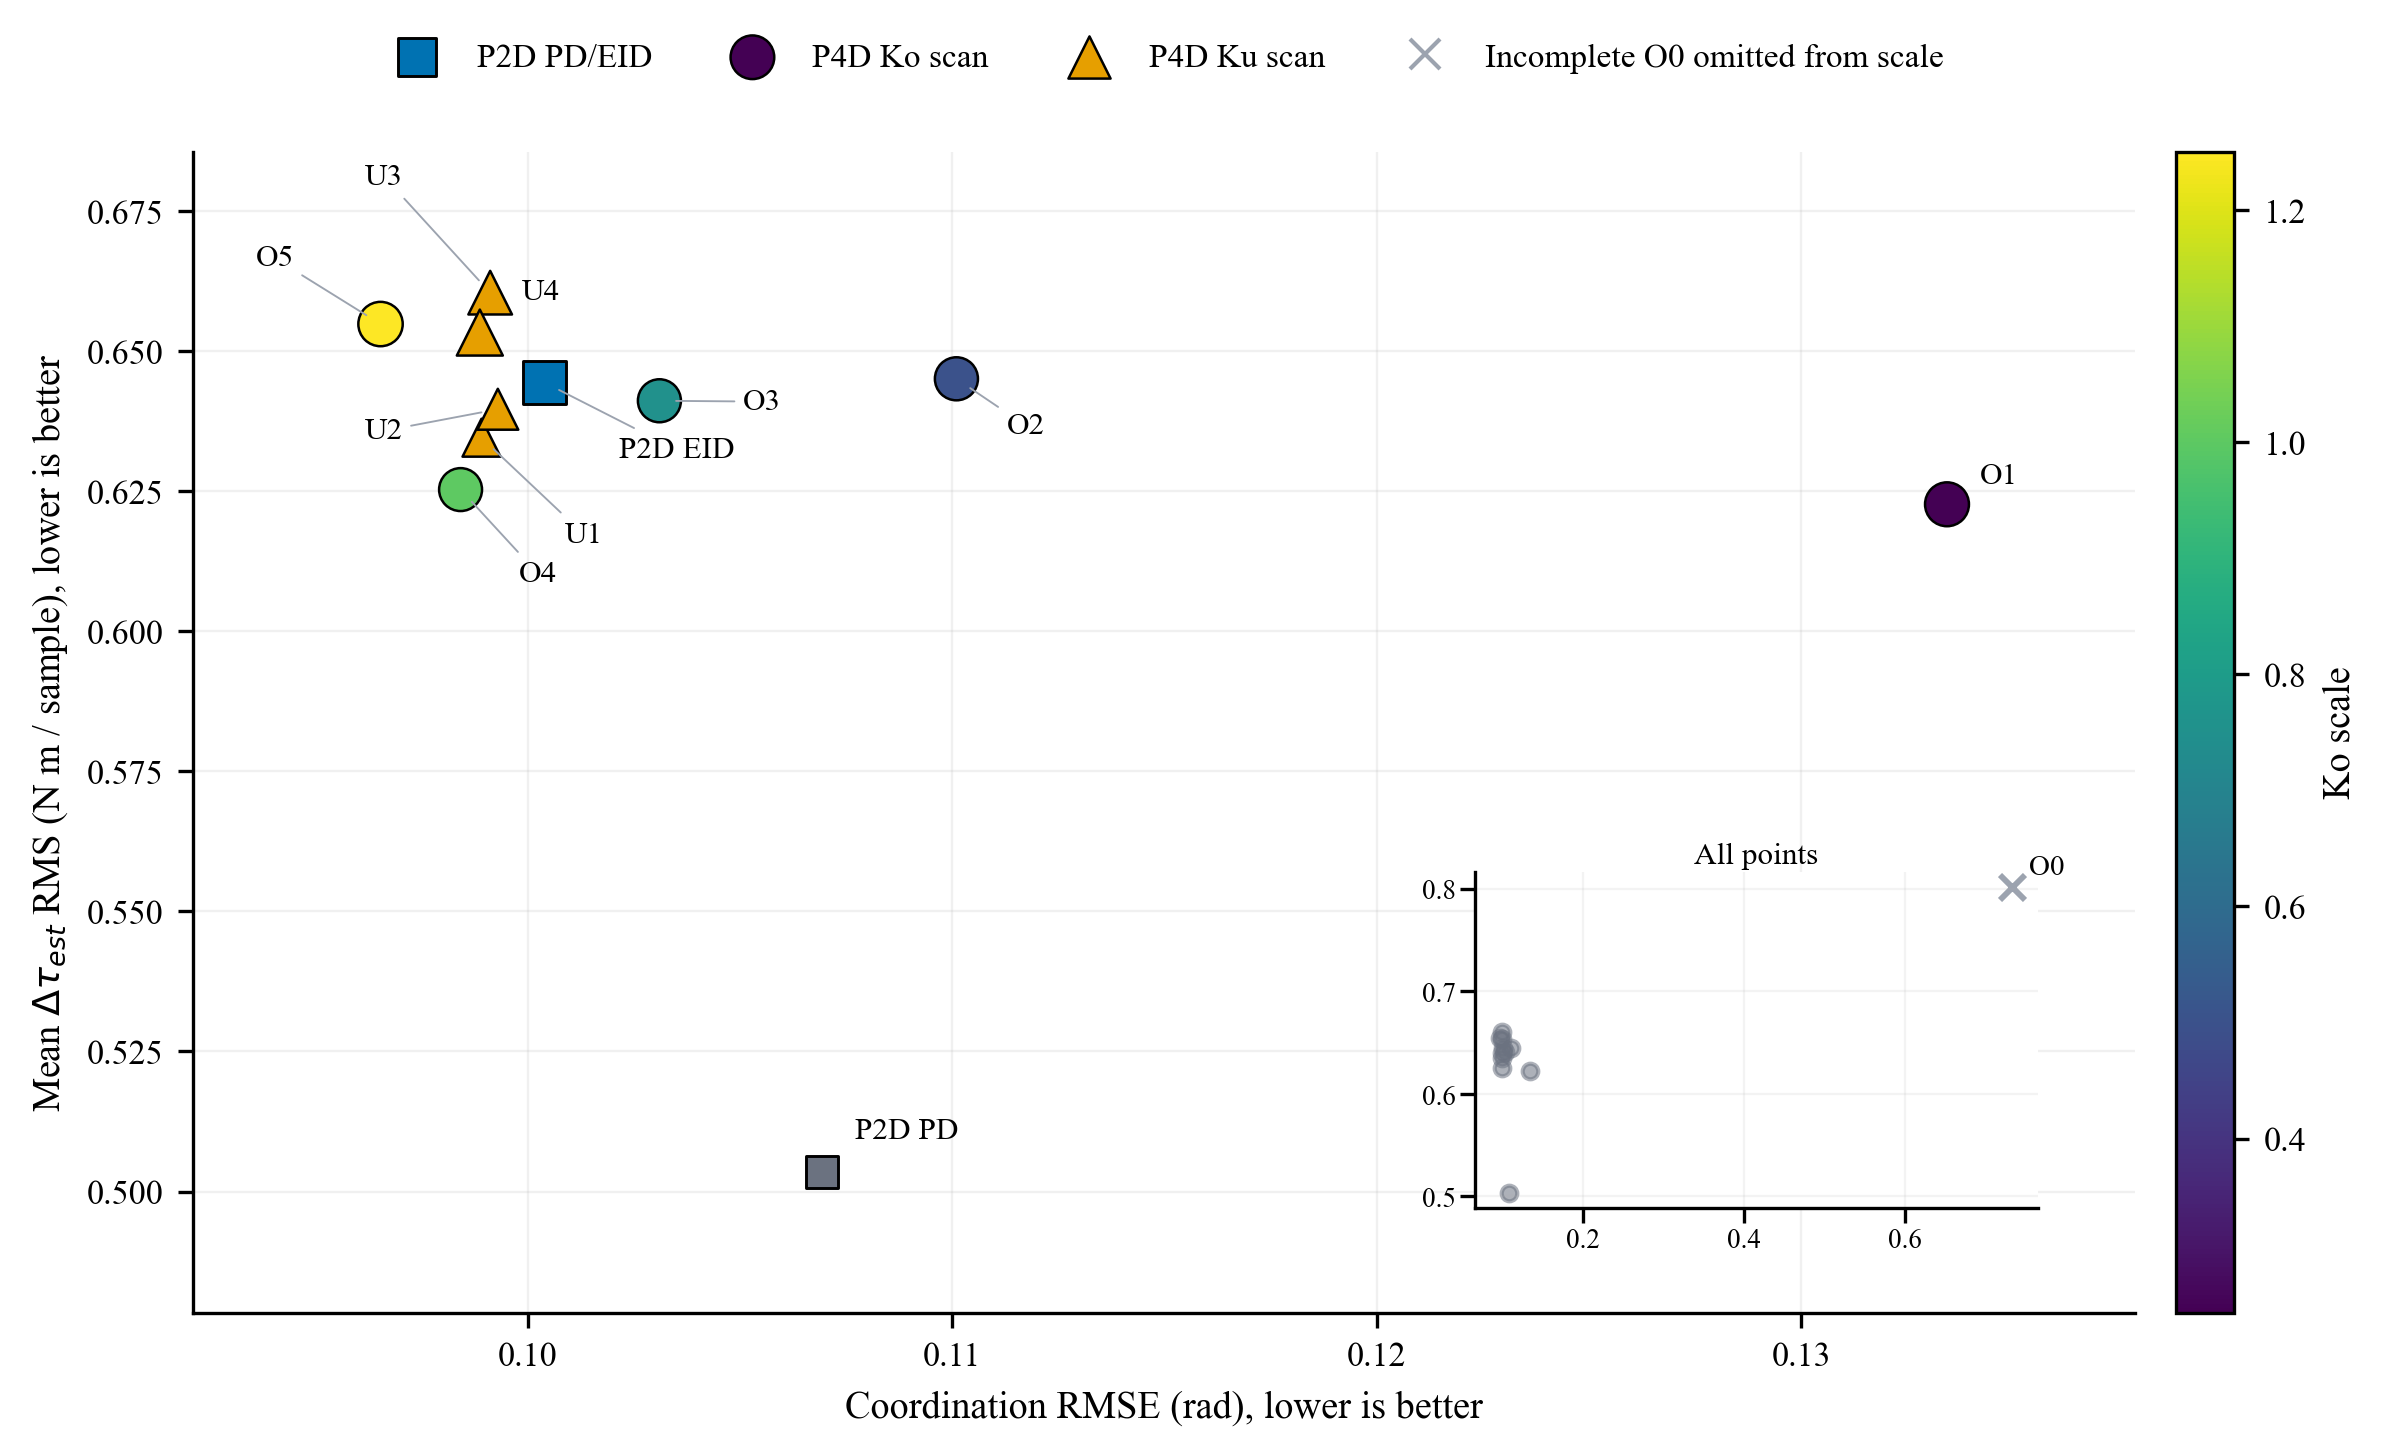
\includegraphics[keepaspectratio,alt={误差收益-力矩代价 Pareto}]{analysis_artifacts/bychen_answer/figures/bychen_tradeoff_pareto.png}}
\caption{实物日志误差-力矩代价 Pareto。横轴为协调 RMSE，纵轴为平均 \(\Delta\tau_{\rm est}\) RMS，点大小表示平均 \(\eta_u\) RMS。参数选择应先看 Pareto 关系和硬约束，而不是只按单一 RMSE 最小化排名。}
\end{figure}

\section{5. 仿真预筛：MuJoCo 用于确定下一轮实机优先级}
\label{sec:mujoco}

本节回答一个很具体的问题：在实机时间和风险都有限的情况下，下一轮应该优先测试哪几组参数。MuJoCo 仿真使用与实机控制器一致的控制计算流程，并施加与 P2D/P4D 相同的软件输入端等效扰动，用来做仿真预筛：先排除明显不值得优先上机的组合，再把剩余候选分成“保守基线”“误差收益候选”和“膝力矩活动机制验证点”。它不能证明某个候选在实机上最优，也不能给出上机安全裕度。本轮所有候选在仿真中都触发同一类风险标记，因此表中只比较误差与力矩趋势，不把仿真排名写成上机安全排序。

\begin{longtable}[]{@{}L{0.25\linewidth}L{0.18\linewidth}rrrr@{}}
\caption{MuJoCo 候选层结果。相对变化均相对 A/\(\mathrm{O4+U1}\)；负值表示下降；表中膝 \(\Delta\tau\) 为膝 \(\Delta\tau_{\rm total}\) RMS。}\\
\toprule
候选 & 角色 & 协调 RMSE & 膝 \(\Delta\tau\) & 协调变化 & 膝 \(\Delta\tau\) 变化 \\
\midrule
\endfirsthead
\toprule
候选 & 角色 & 协调 RMSE & 膝 \(\Delta\tau\) & 协调变化 & 膝 \(\Delta\tau\) 变化 \\
\midrule
\endhead
\bottomrule
\endlastfoot
A：保守基线 \(\mathrm{O4+U1}\) & 保守基线 & 0.067562 & 0.137295 & 0.00\% & 0.00\% \\
B：只提高髋 \(K_o\) & 髋增强候选 & 0.067200 & 0.137283 & -0.54\% & -0.01\% \\
E：共同提高髋膝 \(K_o\) & 误差优先候选 & 0.065995 & 0.138420 & -2.32\% & +0.82\% \\
D：提高髋 \(K_o\)、降低膝 \(K_o\) & 膝机制验证 & 0.069233 & 0.135377 & +2.47\% & -1.40\% \\
只降低膝速度通道 & 膝速度机制验证 & 0.069429 & 0.135514 & +2.76\% & -1.30\% \\
\end{longtable}

\begin{figure}[H]
\centering
\pandocbounded{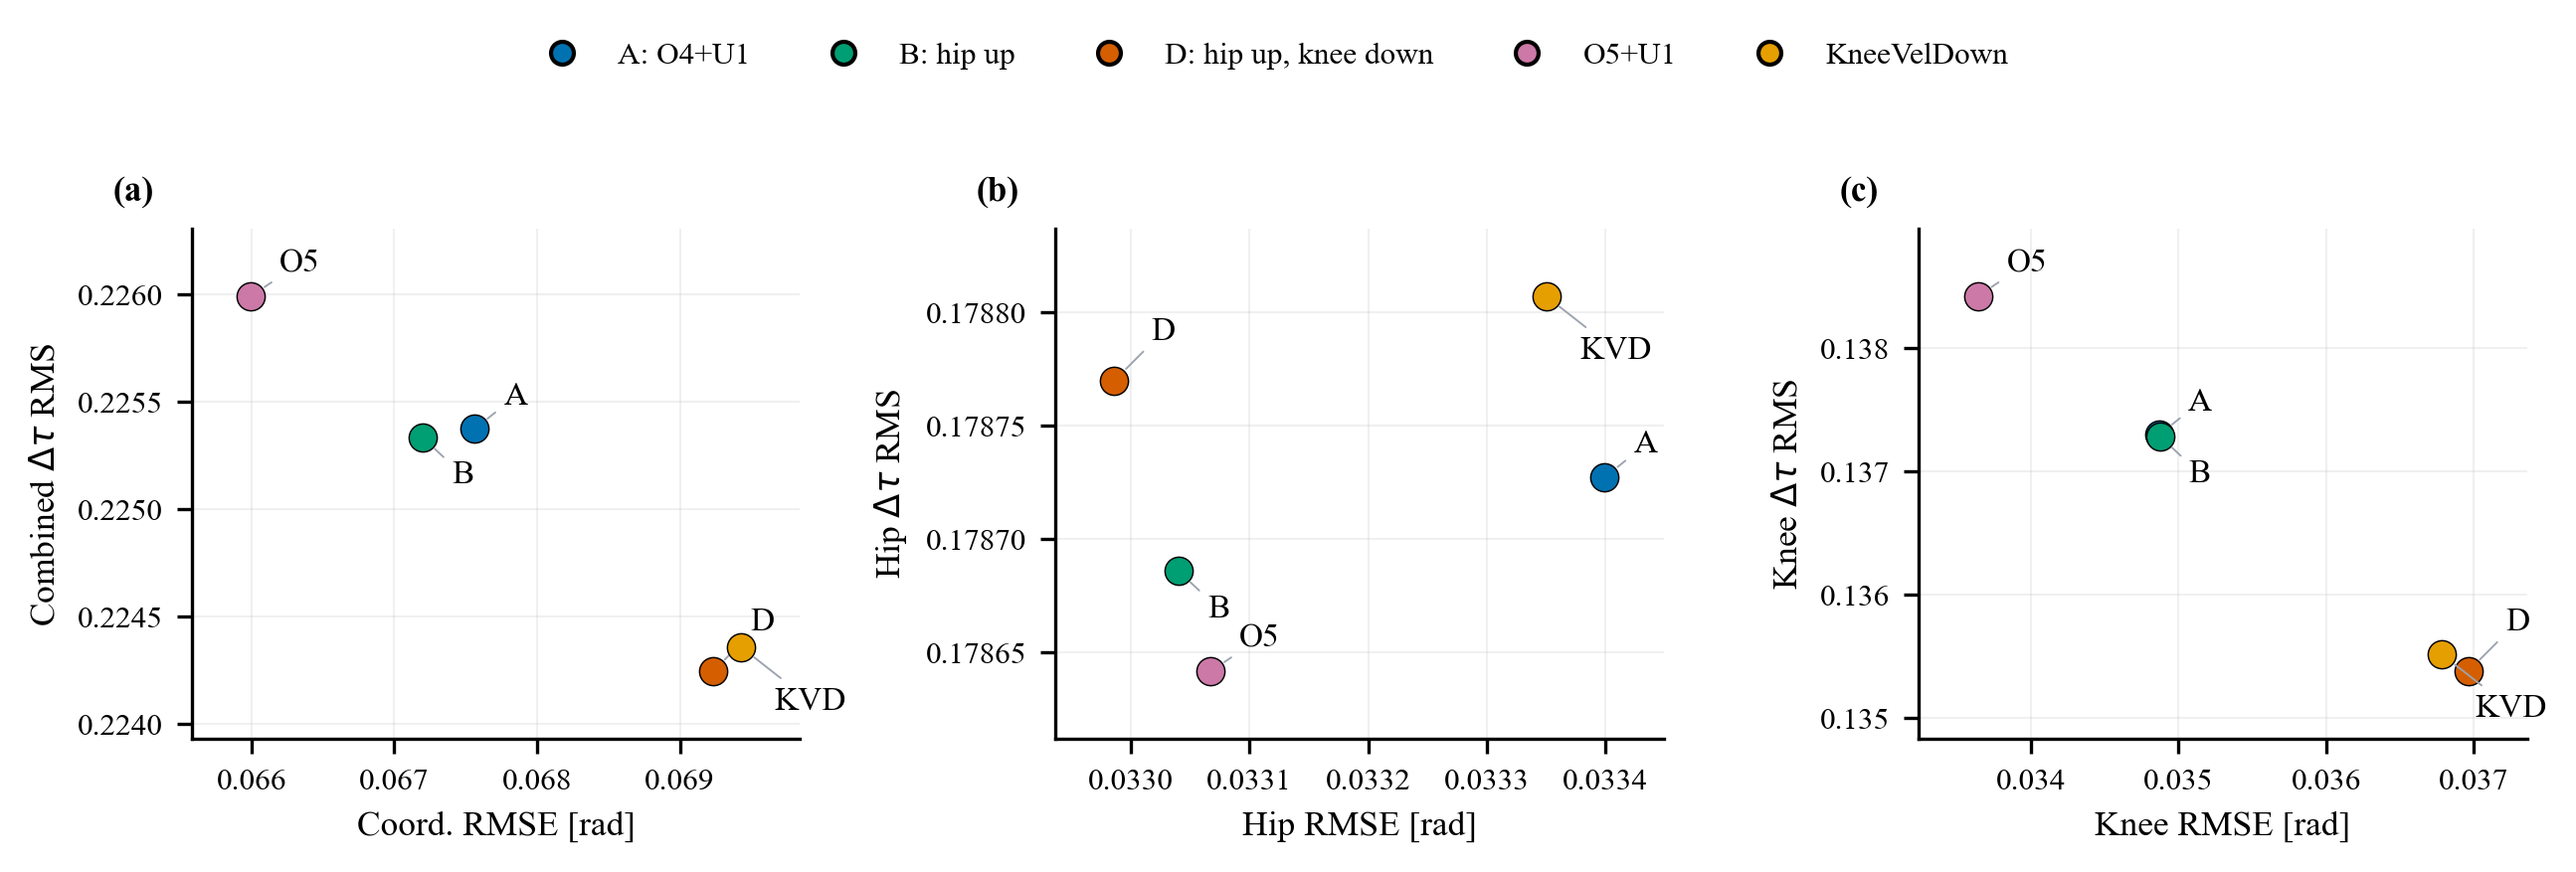
\includegraphics[keepaspectratio,alt={MuJoCo 机制矩阵候选 Pareto}]{analysis_artifacts/bychen_mujoco_mechanism_completion/figures/mujoco_mechanism_candidate_pareto.png}}
\caption{MuJoCo 机制矩阵候选 Pareto。B 和 E 用于误差收益验证；D 与“只降低膝速度通道”用于膝力矩活动机制验证。该图不支持把这些膝通道候选预写成最优候选。}
\end{figure}

这组结果给出三个候选角色。A 是已有实机依据的保守基线。B 是低风险误差收益候选，因为协调 RMSE 只下降约 0.54\%，但膝力矩变化量几乎不变。E 是误差优先候选，因为协调 RMSE 下降约 2.32\%，但膝 \(\Delta\tau_{\rm total}\) RMS 上升约 0.82\%，且组合本身尚未实机验证。提高髋 \(K_o\) 同时降低膝 \(K_o\)、或只降低膝速度通道，更适合作为膝力矩活动机制验证点，因为它们降低膝力矩变化量约 1.3\%--1.4\%，但协调 RMSE 变差约 2.5\%--2.8\%。

\begin{figure}[H]
\centering
\pandocbounded{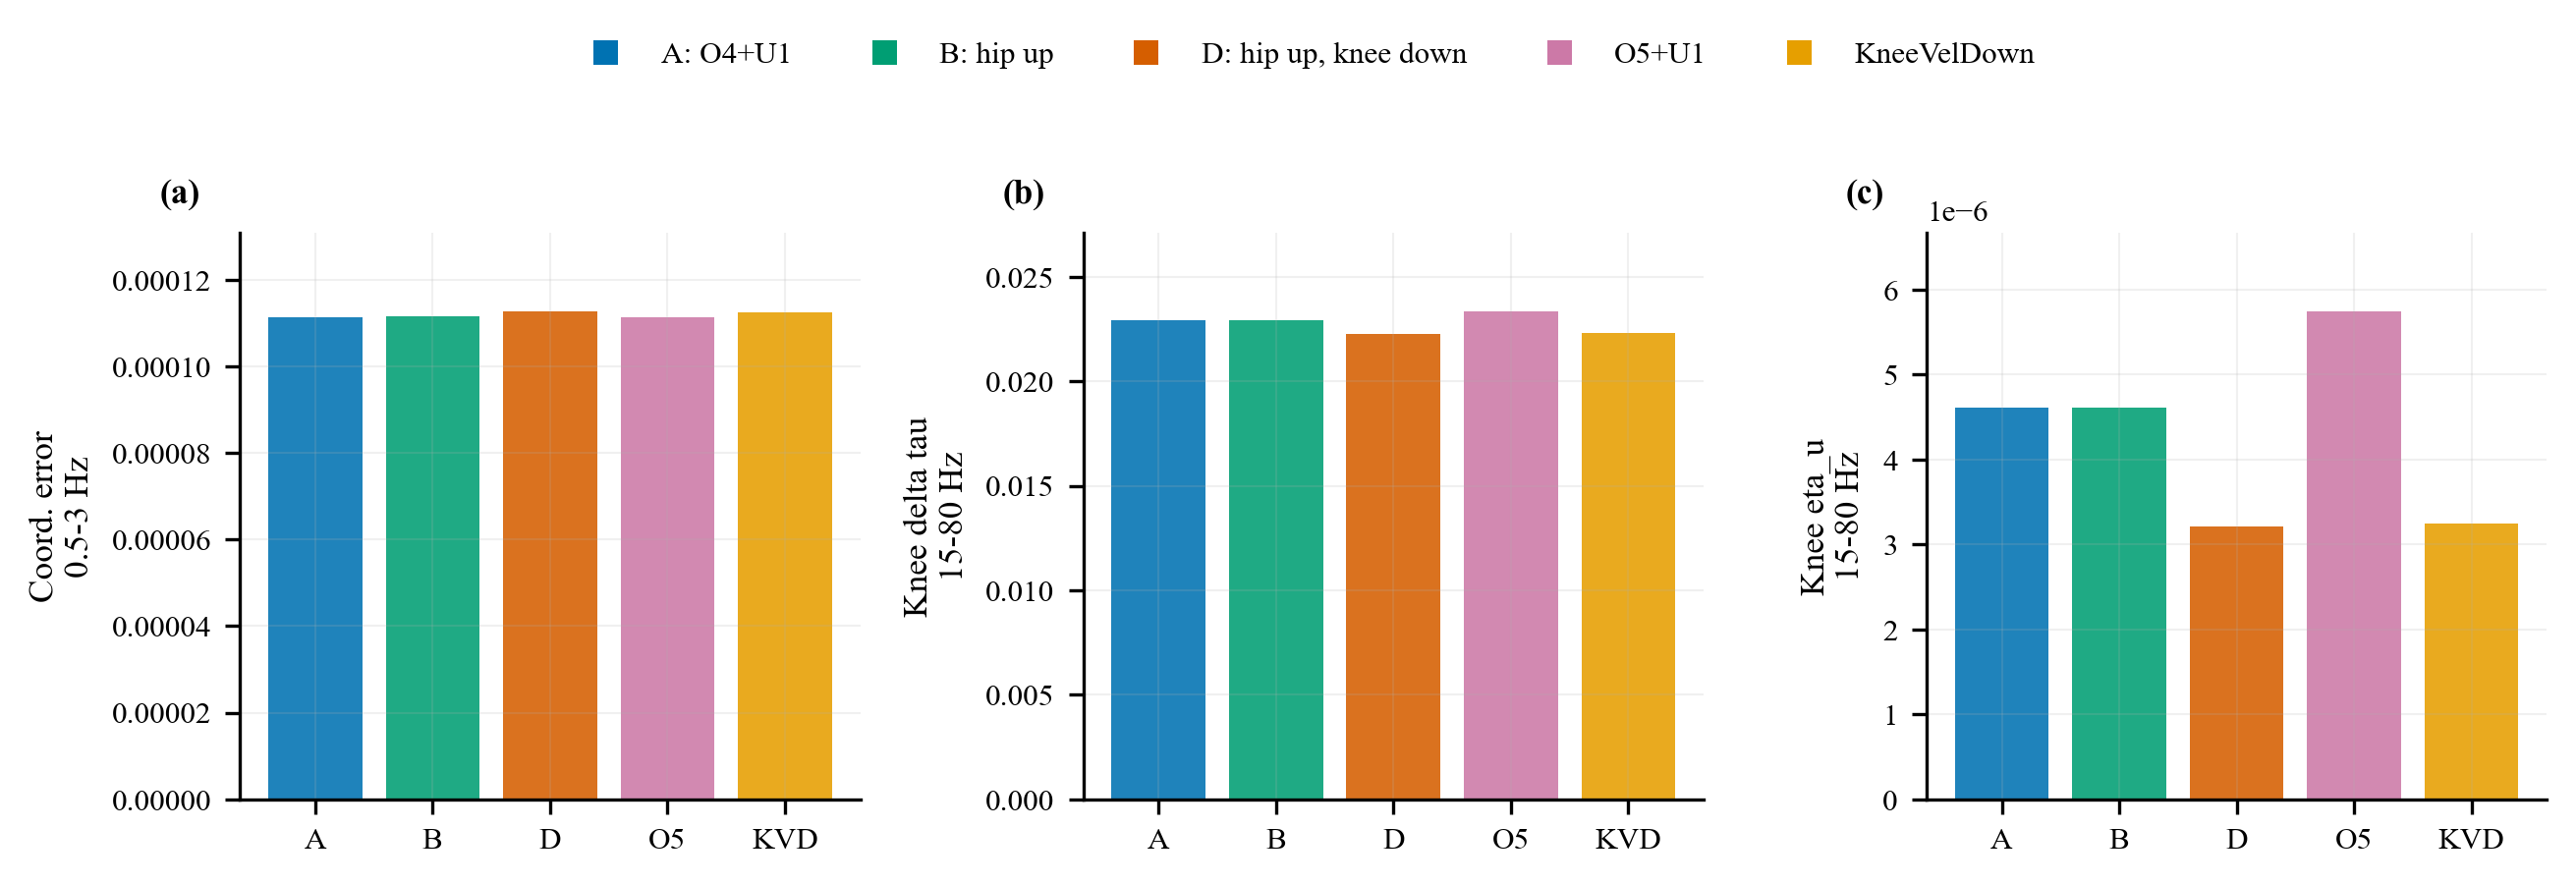
\includegraphics[keepaspectratio,alt={MuJoCo 机制矩阵频谱摘要}]{analysis_artifacts/bychen_mujoco_mechanism_completion/figures/mujoco_mechanism_spectrum_summary.png}}
\caption{MuJoCo 机制矩阵频谱摘要。提高观测器倍率更偏向误差收益，降低膝速度或膝观测器倍率更偏向膝力矩活动约束；二者在当前数据里不能同时最优。}
\end{figure}

\section{6. 下一轮实验设计}
\label{sec:next}

下一轮实验应从``继续扫更大的 O 或 U''转为假设判别：复测保守基线，验证两个误差收益候选，再用膝通道候选检查力矩活动机制。所有 EID 候选默认固定弱输入补偿：

\[
s_{u,h}=s_{u,k}=0.5,\qquad \alpha=0.85.
\]

\subsection{6.1 同批实机复测矩阵}

\begin{longtable}[]{@{}L{0.12\linewidth}L{0.20\linewidth}cL{0.16\linewidth}L{0.39\linewidth}@{}}
\caption{下一轮第一优先级实机矩阵。每组先做无扰动门槛，再做 P2D 软件输入端扰动，每组至少 5 次完整重复。}\\
\toprule
优先级 & 候选 & 髋 \(s_o\) & 膝 \(s_o\) & 回答的问题 \\
\midrule
\endfirsthead
\toprule
优先级 & 候选 & 髋 \(s_o\) & 膝 \(s_o\) & 回答的问题 \\
\midrule
\endhead
\bottomrule
\endlastfoot
必做 & A / \(\mathrm{O4+U1}\) & 1.00 & 1.00 & 保守基线是否可在同批次复现 \\
必做 & B：只提高髋 \(K_o\) & 1.25 & 1.00 & 只提高髋 \(K_o\) 是否带来更稳妥的误差收益 \\
必做 & E / \(\mathrm{O5+U1}\) & 1.25 & 1.25 & 共同高 \(K_o\) + 弱 \(K_u\) 是否真的优于 A \\
机制验证 & C：只降低膝 \(K_o\) & 1.00 & 0.75 & 单独降低膝 \(K_o\) 的代价和收益 \\
机制验证 & D：提高髋 \(K_o\)、降低膝 \(K_o\) & 1.25 & 0.75 & 直接检验``髋增、膝减''假设 \\
机制验证 & 只降低膝速度通道 & 1.00 & 膝位置 1.00，膝速度 0.75 & 膝力矩活动是否主要来自速度残差通道 \\
\end{longtable}

如果上机时间有限，先做 A/B/E；若必须直接回答非对称调参问题，则执行 A/B/C/D 的最小 2x2 矩阵。每组必须报告髋/膝/协调窗口 RMSE、峰值误差、恢复段 RMSE、恢复时间、\(\tau_{\rm est}\) RMS、\(\Delta\tau_{\rm est}\) RMS、分频段力矩功率、饱和次数、速度超限和完整运行率。

\subsection{6.3 真实物理外扰验证}

P2D/P4D 的软件扰动是在命令侧叠加的输入端等效扰动，不能替代真实外部物理接触力。下一轮如果要回答真实外扰抗扰能力，必须引入可测外力方式，例如带力传感器的加载装置或已知加载机构。需要检验的假设包括：真实外扰是否仍主要通过状态误差进入 \(\bar{x}\)/反馈中心；接触冲击是否使 \(\eta\) 更像噪声或冲击滤波状态；Preview-MPC 对真实外扰的帮助是否有限，因为它主要降低参考激励而不直接处理接触冲击。

\clearpage
\section{附录 A：频谱、恢复段与图表索引}
\label{sec:appendix-figures}

正文只保留会改变决策的问题。下面图表用于复核频谱、恢复段和候选差异来源。

\begin{figure}[H]
\centering
\pandocbounded{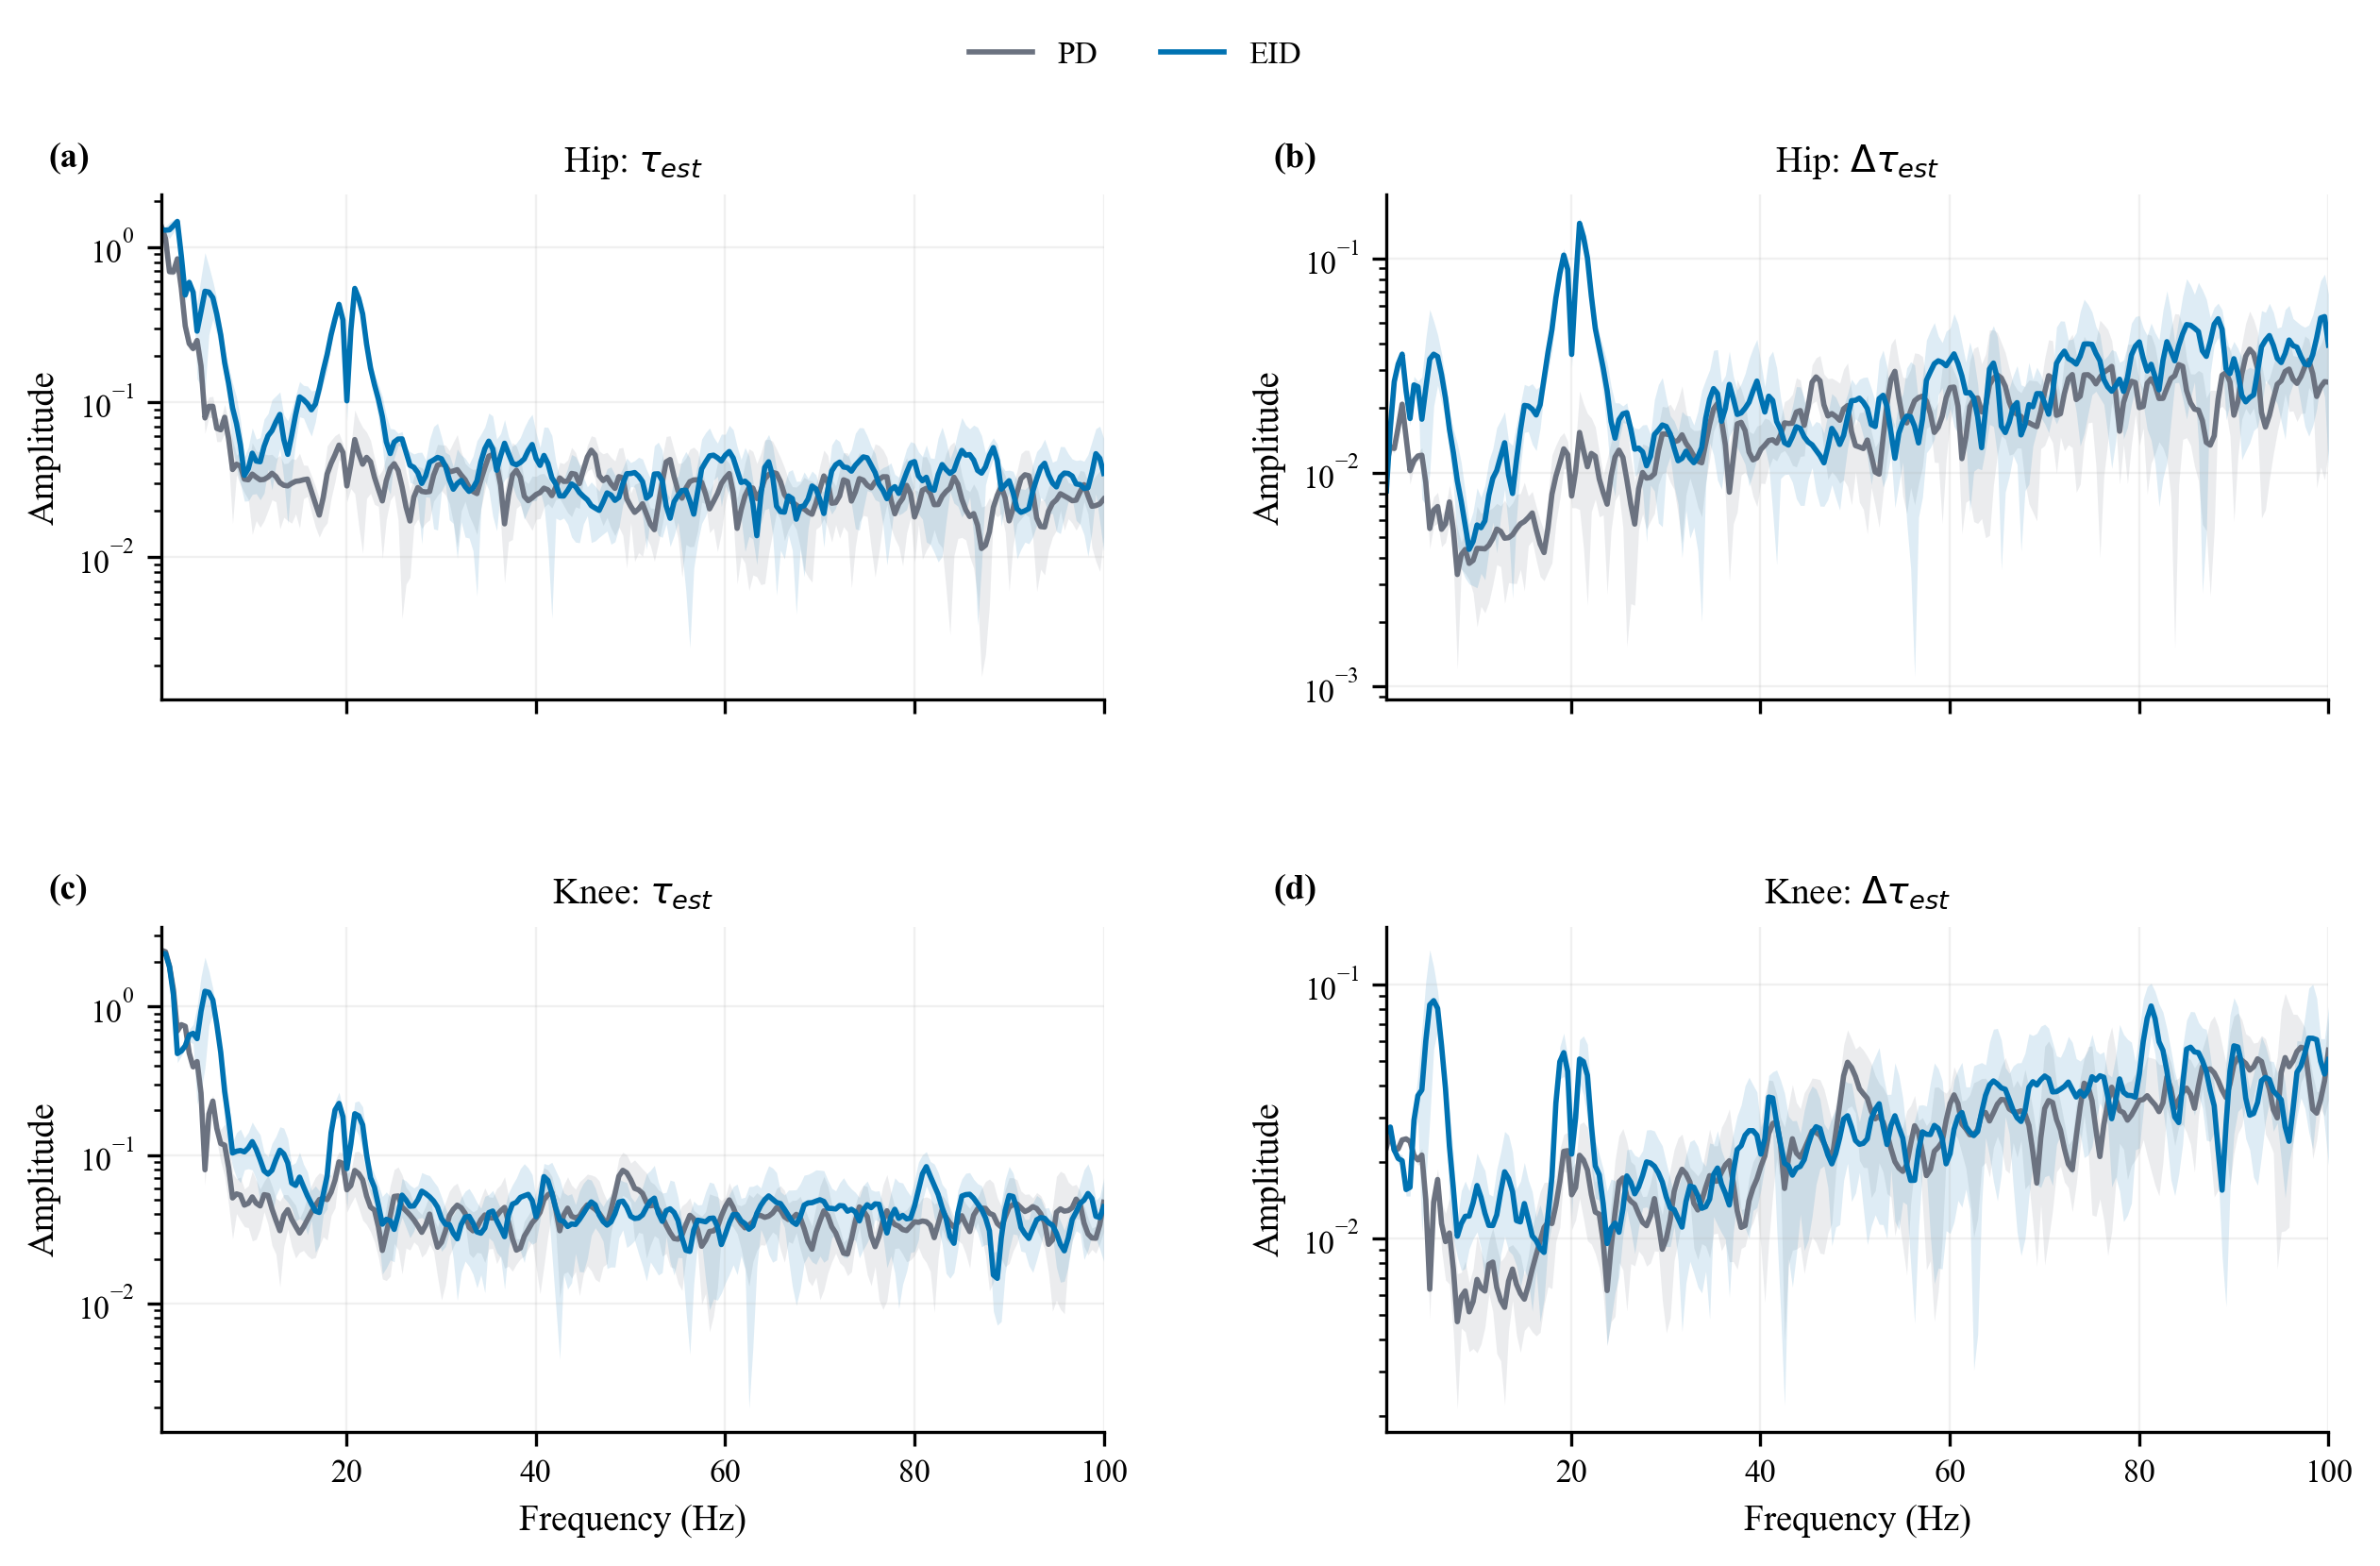
\includegraphics[keepaspectratio,alt={P2D 全重复频谱}]{analysis_artifacts/bychen_answer/figures/bychen_p2d_all_repeat_spectrum.png}}
\caption{P2D 全重复频谱。EID 的力矩活动增加不是单一 RMSE 指标能描述的现象，需要与频段和恢复段一起阅读。}
\end{figure}

\begin{figure}[H]
\centering
\pandocbounded{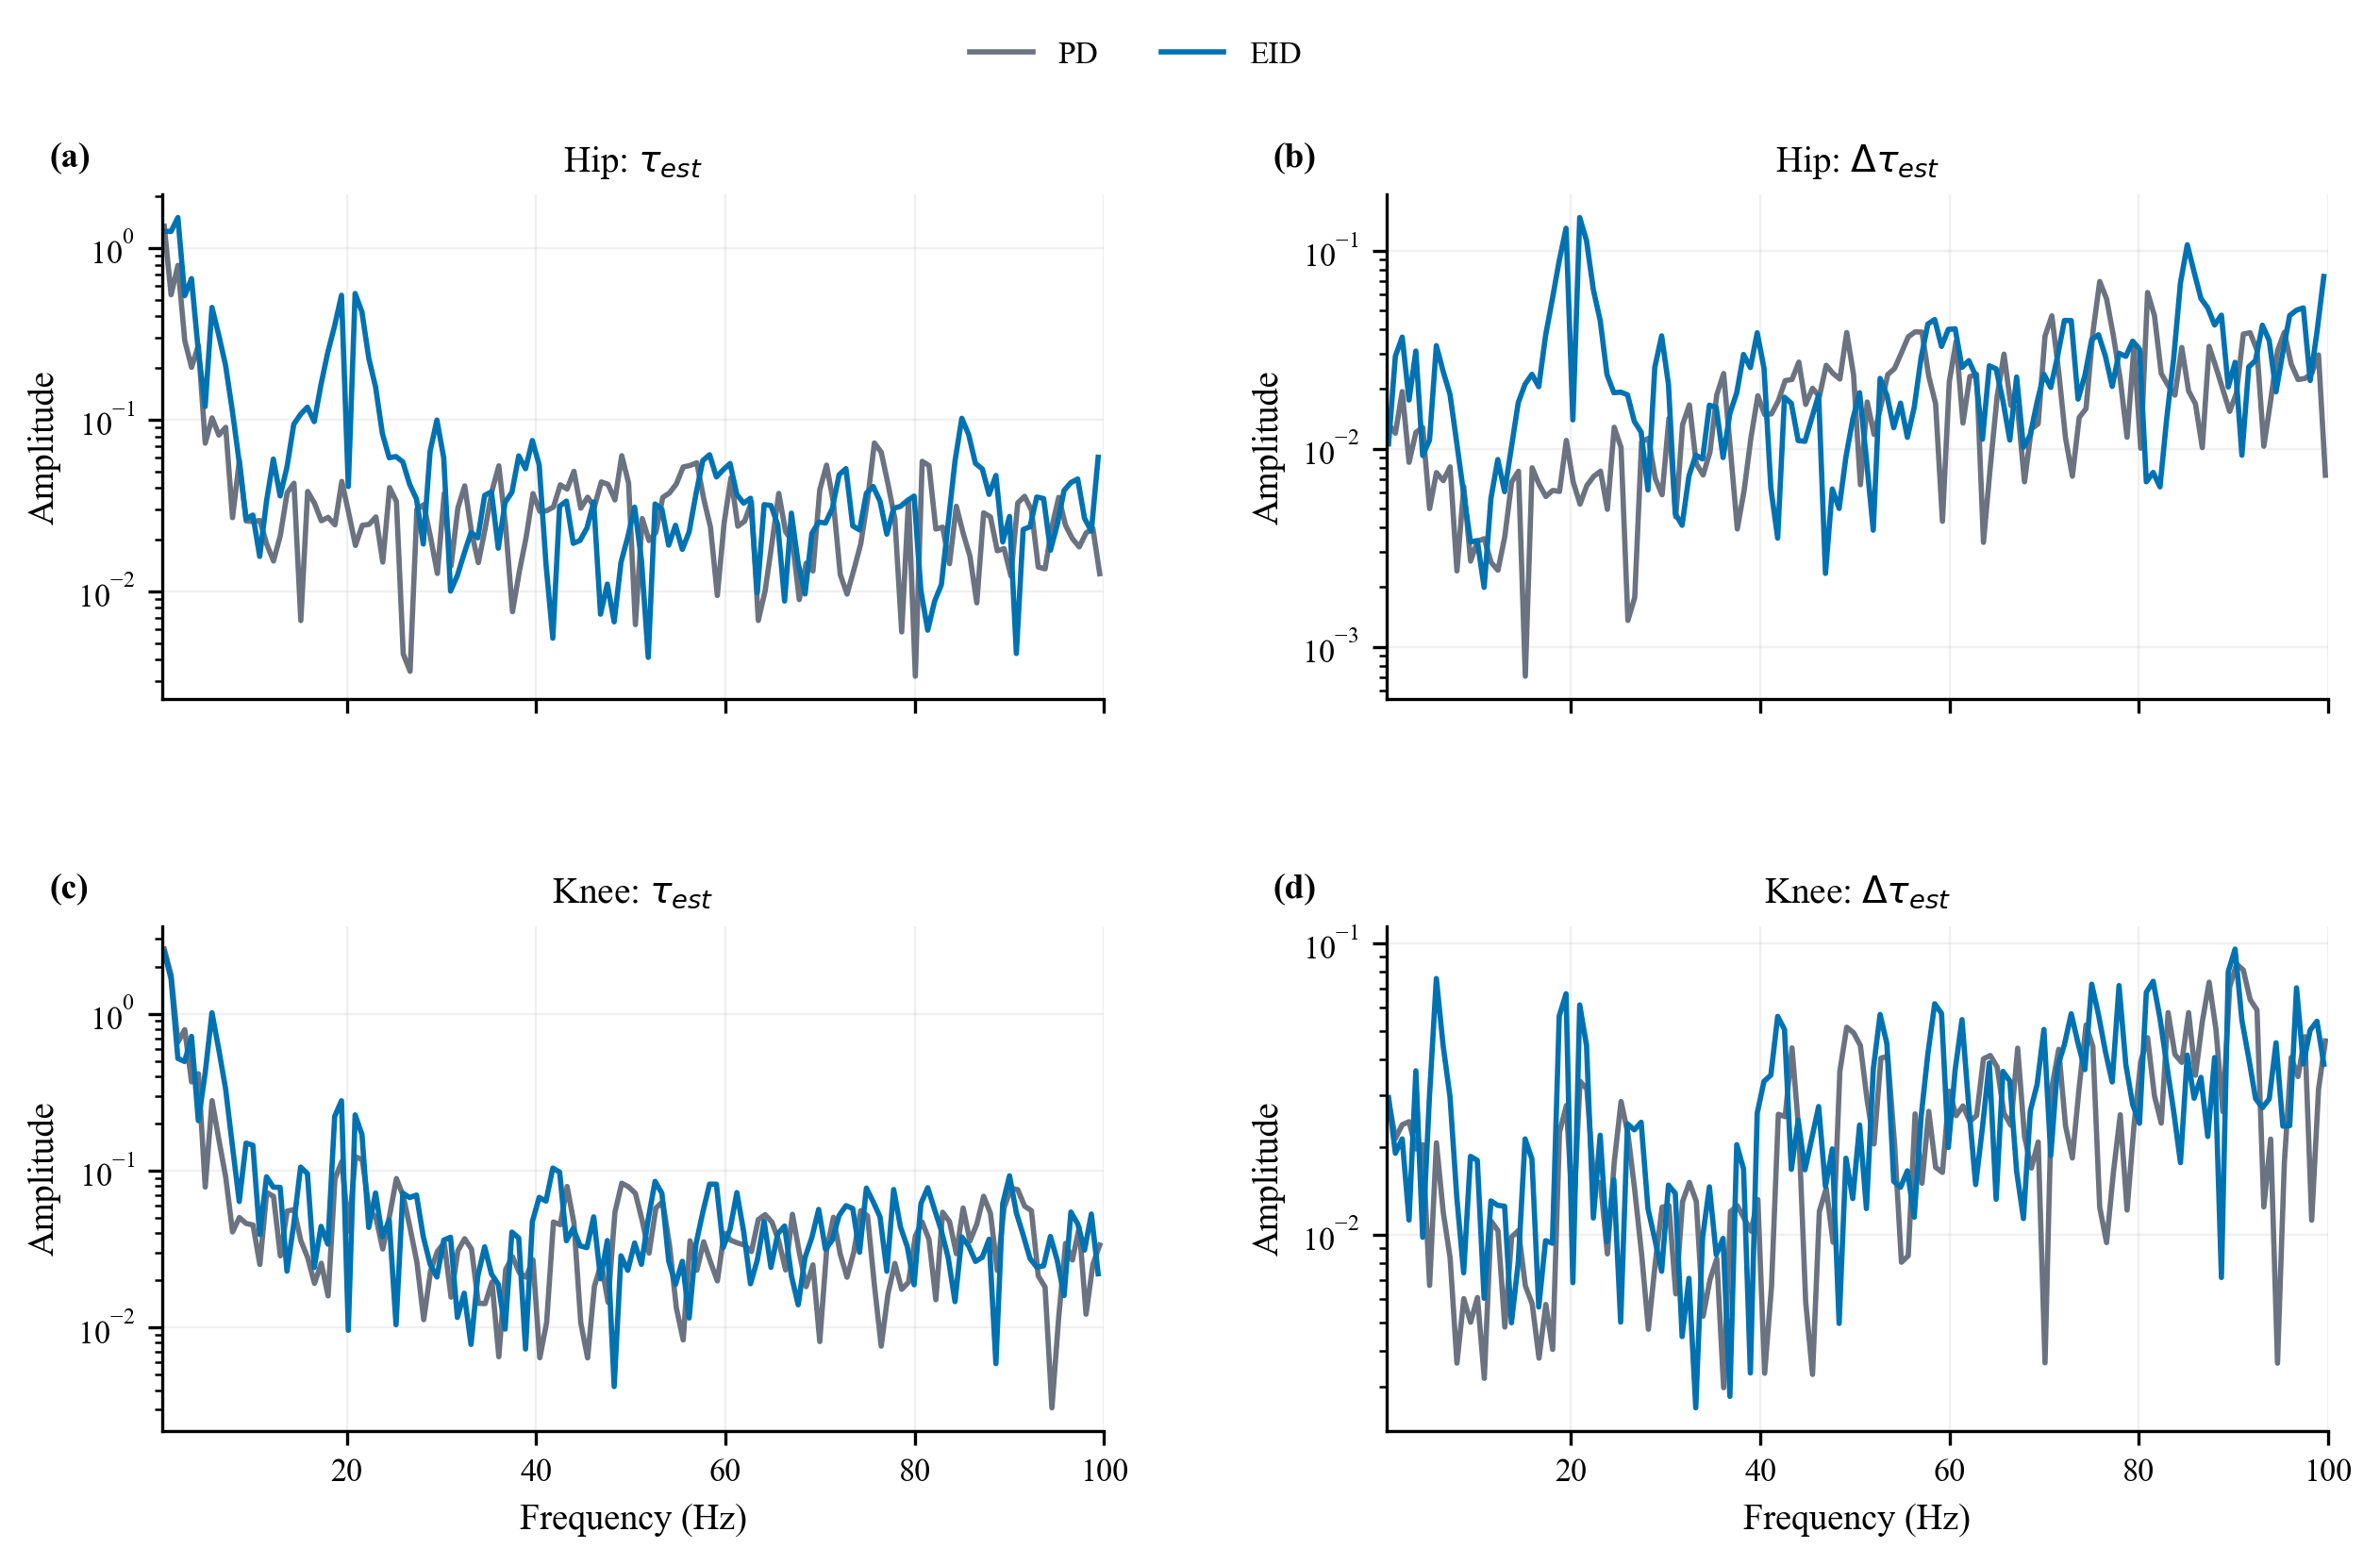
\includegraphics[keepaspectratio,alt={P2D 扰动窗口频谱}]{analysis_artifacts/bychen_answer/figures/bychen_p2d_disturbance_spectrum.png}}
\caption{P2D 扰动窗口频谱。该图用于区分窗口内误差响应和力矩活动的频率分布。}
\end{figure}

\begin{figure}[H]
\centering
\pandocbounded{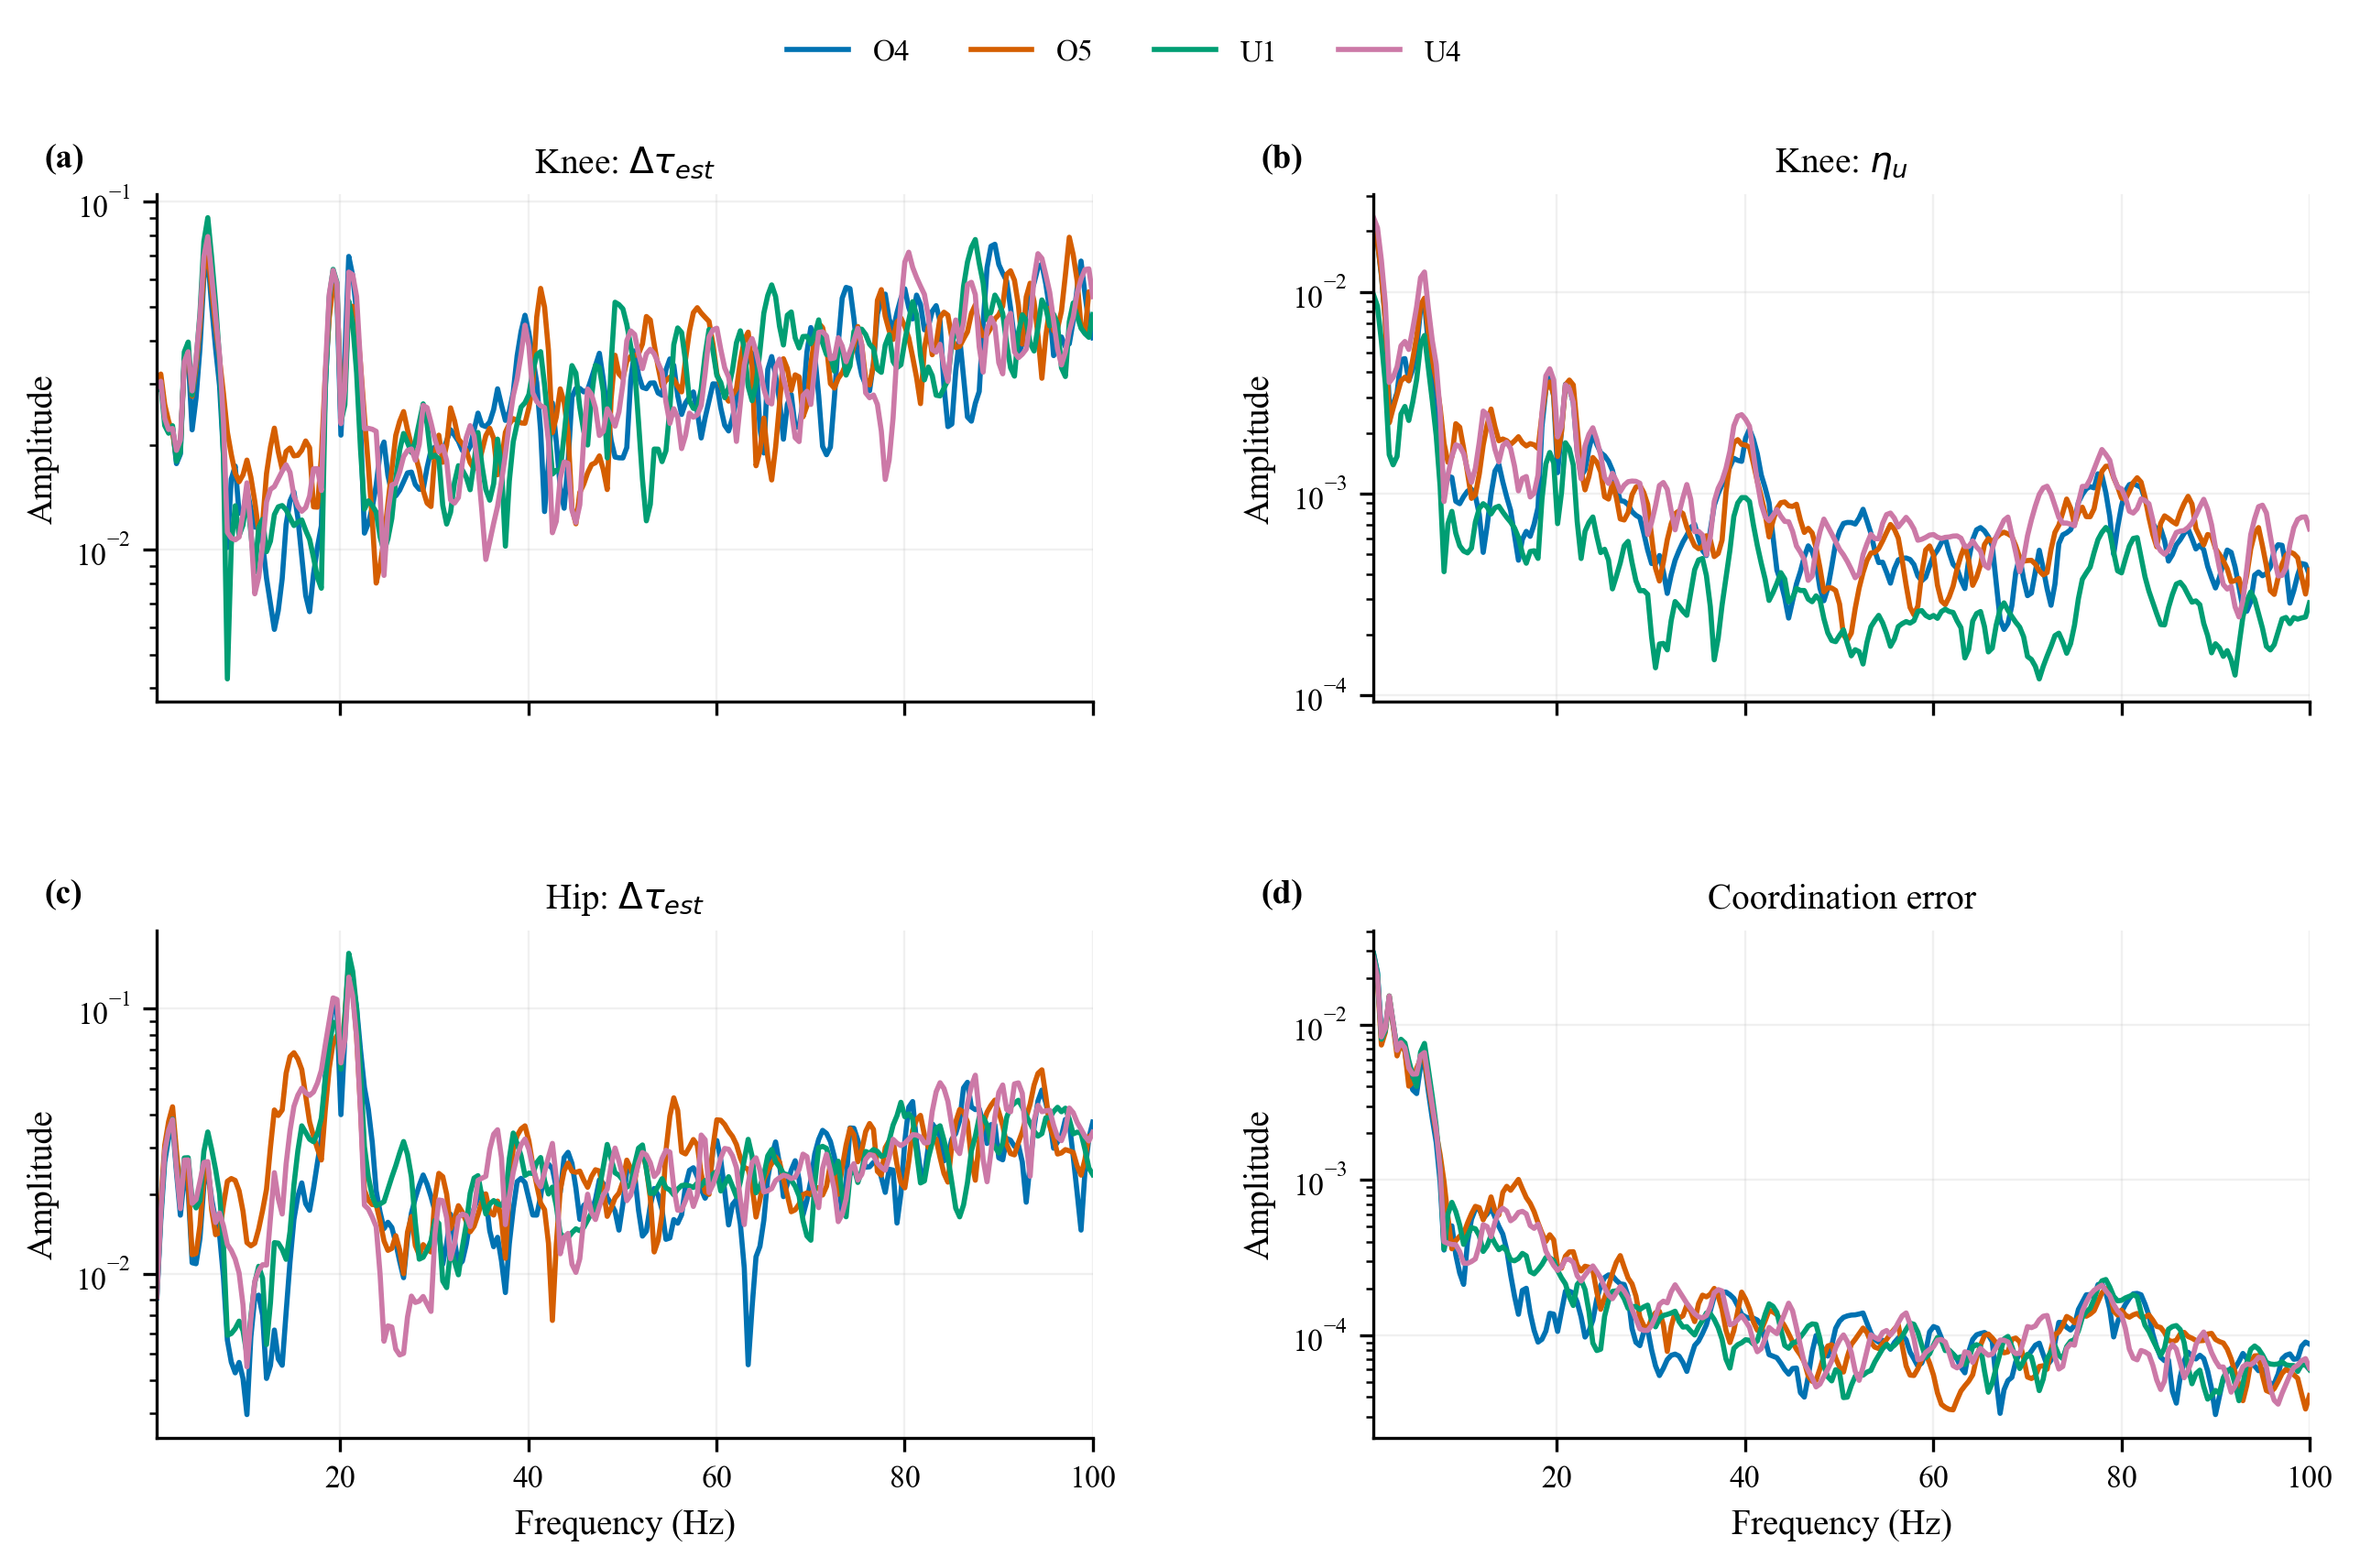
\includegraphics[keepaspectratio,alt={P4D 候选频谱}]{analysis_artifacts/bychen_answer/figures/bychen_p4d_candidate_spectrum.png}}
\caption{P4D O4/O5/U1/U4 候选频谱。O5 的协调误差频谱略低，但局部 \(\eta_u\) 和力矩高频活动更强；U1 是更保守的补偿基线。}
\end{figure}

\begin{figure}[H]
\centering
\pandocbounded{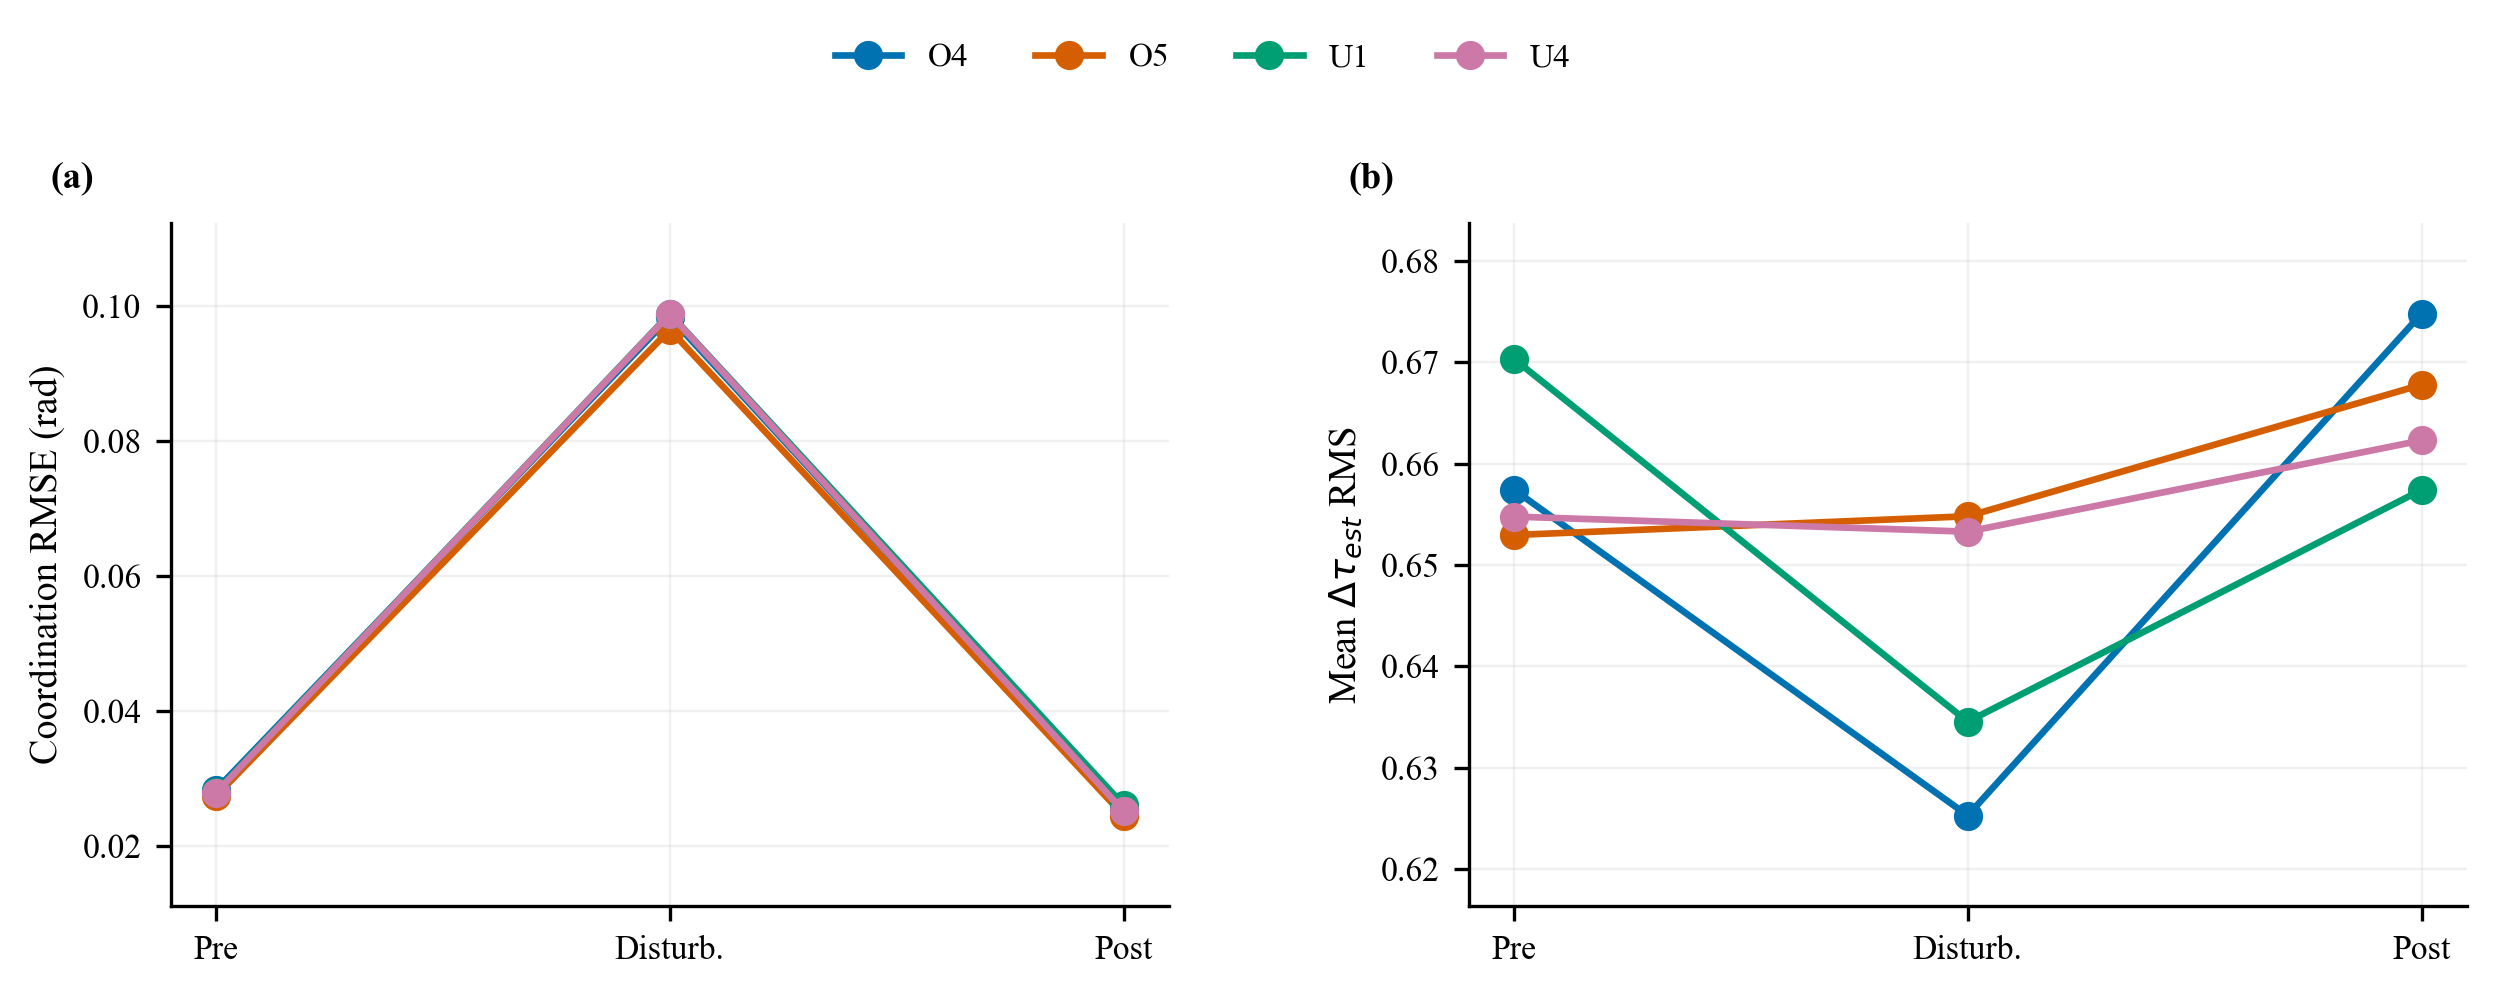
\includegraphics[keepaspectratio,alt={P4D 候选窗口统计}]{analysis_artifacts/bychen_answer/figures/bychen_p4d_candidate_windows.png}}
\caption{P4D 候选窗口统计。该图用于复核扰动前、扰动窗口和恢复段的候选差异。}
\end{figure}

\section{附录 B：MuJoCo 日志频谱与局部模型}
\label{sec:appendix-models}

本附录解释第 5 节中 MuJoCo 仿真预筛背后的频域和局部模型分析。这里有两层分析。第一层直接使用 MuJoCo 日志，计算功率谱密度（PSD）、扰动与响应之间的 coherence，以及经验频响函数（FRF）。它回答的问题是：扰动、误差和力矩活动主要集中在哪些频段，不同候选的频域行为是否一致。第二层先从 MuJoCo 日志辨识一个局部离散时间关节模型，再把 EID 的预测状态、内部状态和输入补偿更新写进增广闭环矩阵。它回答的问题是：在这个局部线性近似里，候选之间的极点、扰动到误差频响、测量噪声到控制输出放大趋势有什么差别。

这两层分析的作用都是解释候选差异来源，而不是证明实机稳定性。原因有三点。第一，MuJoCo 中使用的是软件输入端等效扰动，不是真实外部接触力。第二，离散时间增广模型是围绕当前日志工作点辨识得到的局部线性模型，不等同于完整非线性机器人。第三，频响和极点只覆盖辨识窗口、候选参数和当前扰动形式。因此，下面的图可以支持“哪个候选更值得上机验证”或“差异可能来自哪条通道”，但不能写成“实机全局稳定”或“实机安全裕度已经验证”。

局部离散时间模型的基本形式是：

\[
x_{k+1}=A x_k+B u_k,
\qquad x_k=[q_k,\dot q_k]^\top .
\]

其中 \(q_k\) 和 \(\dot q_k\) 分别是关节位置和速度，\(u_k\) 是该关节总力矩。辨识后，再把 EID 控制器的内部量并入增广状态：

\[
x^{\rm aug}_k=\left[x_k,\hat{x}_k,\eta_k,z_{1,k},\ldots,z_{m,k}\right]^\top .
\]

这里 \(\hat{x}_k\) 是标称预测状态，\(\eta_k\) 是 EID 内部状态，\(z_{i,k}\) 是用于表示采样/计算延迟的历史状态。增广闭环写成：

\[
x^{\rm aug}_{k+1}
=A_{\rm cl}x^{\rm aug}_k+B_d d_k+B_v v_k .
\]

\(d_k\) 表示输入端等效扰动，\(v_k\) 表示测量噪声。本文只读两个输出通道：一个是扰动到位置误差 \(d\rightarrow e_q\)，用于看扰动抑制趋势；另一个是测量噪声到控制输出 \(v\rightarrow u\)，用于看噪声是否容易被放大成力矩活动。

下面各图的读法如下：PSD 看能量集中在哪些频段；coherence 看扰动和响应在某一频段是否具有可解释的线性相关；经验 FRF/Bode 看扰动输入到误差输出的幅值和相位趋势；\(z\) 平面极点看局部离散模型中极点是否接近单位圆；奇异值图看测量噪声进入控制输出时的最大放大趋势。

\begin{figure}[H]
\centering
\pandocbounded{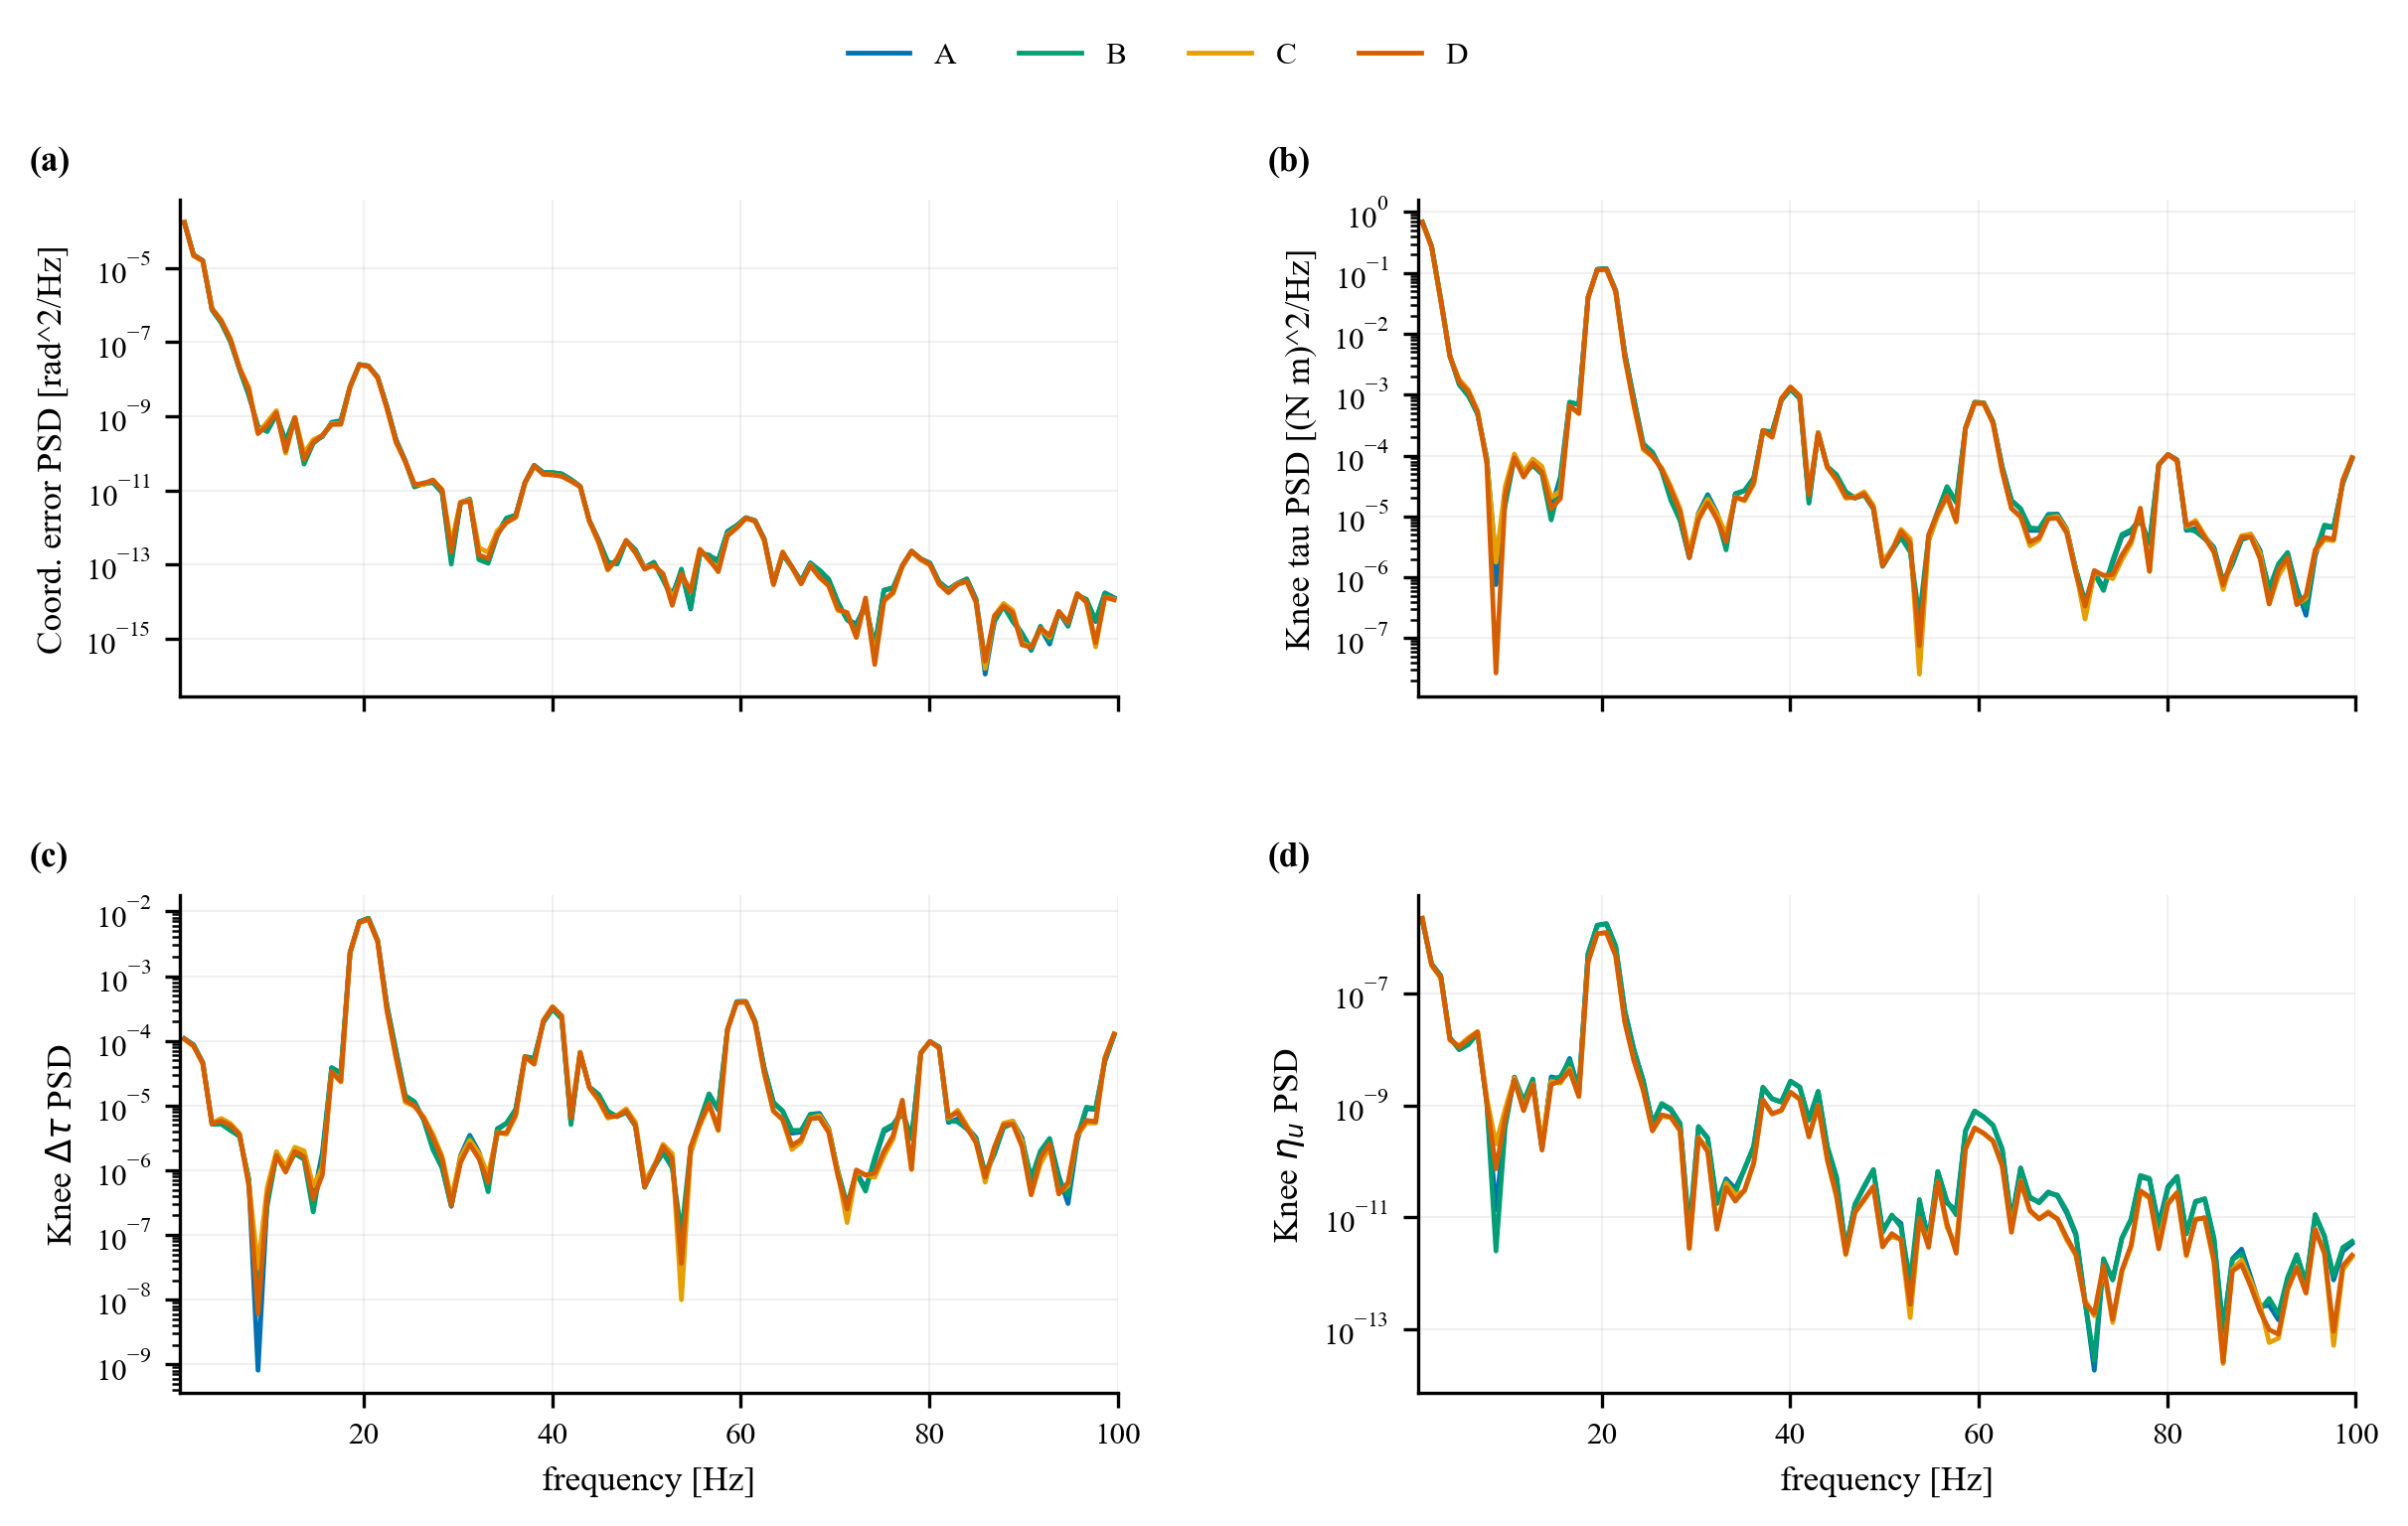
\includegraphics[keepaspectratio,alt={MuJoCo 日志 PSD}]{analysis_artifacts/bychen_mujoco_sweep/mujoco_deep_analysis/figures/bychen_mujoco_log_psd.png}}
\caption{MuJoCo A-D 日志 PSD。该图用于观察候选间误差和力矩活动的频谱差异。}
\end{figure}

\begin{figure}[H]
\centering
\pandocbounded{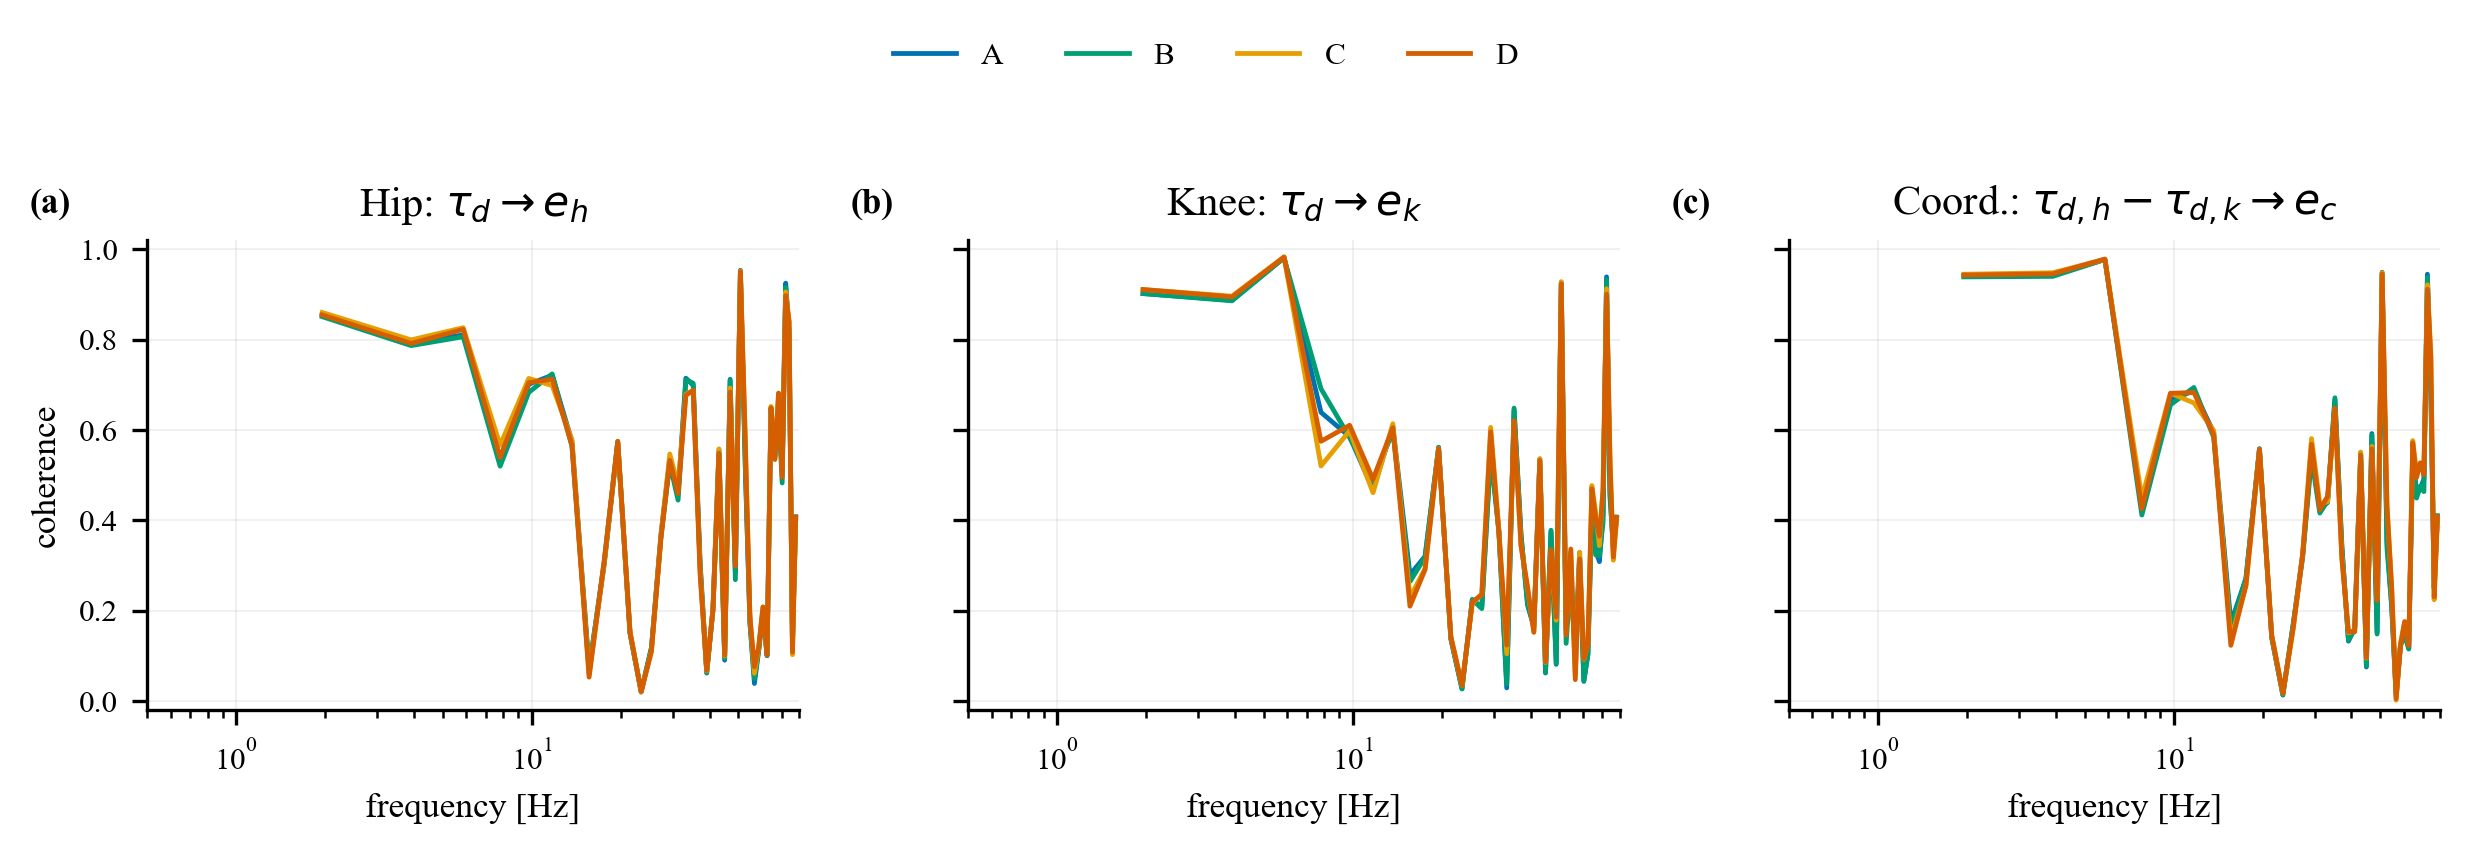
\includegraphics[keepaspectratio,alt={MuJoCo 扰动 coherence}]{analysis_artifacts/bychen_mujoco_sweep/mujoco_deep_analysis/figures/bychen_mujoco_disturbance_coherence.png}}
\caption{MuJoCo 扰动 coherence。该图用于判断扰动输入与误差/力矩信号之间的线性相关频段。}
\end{figure}

\begin{figure}[H]
\centering
\pandocbounded{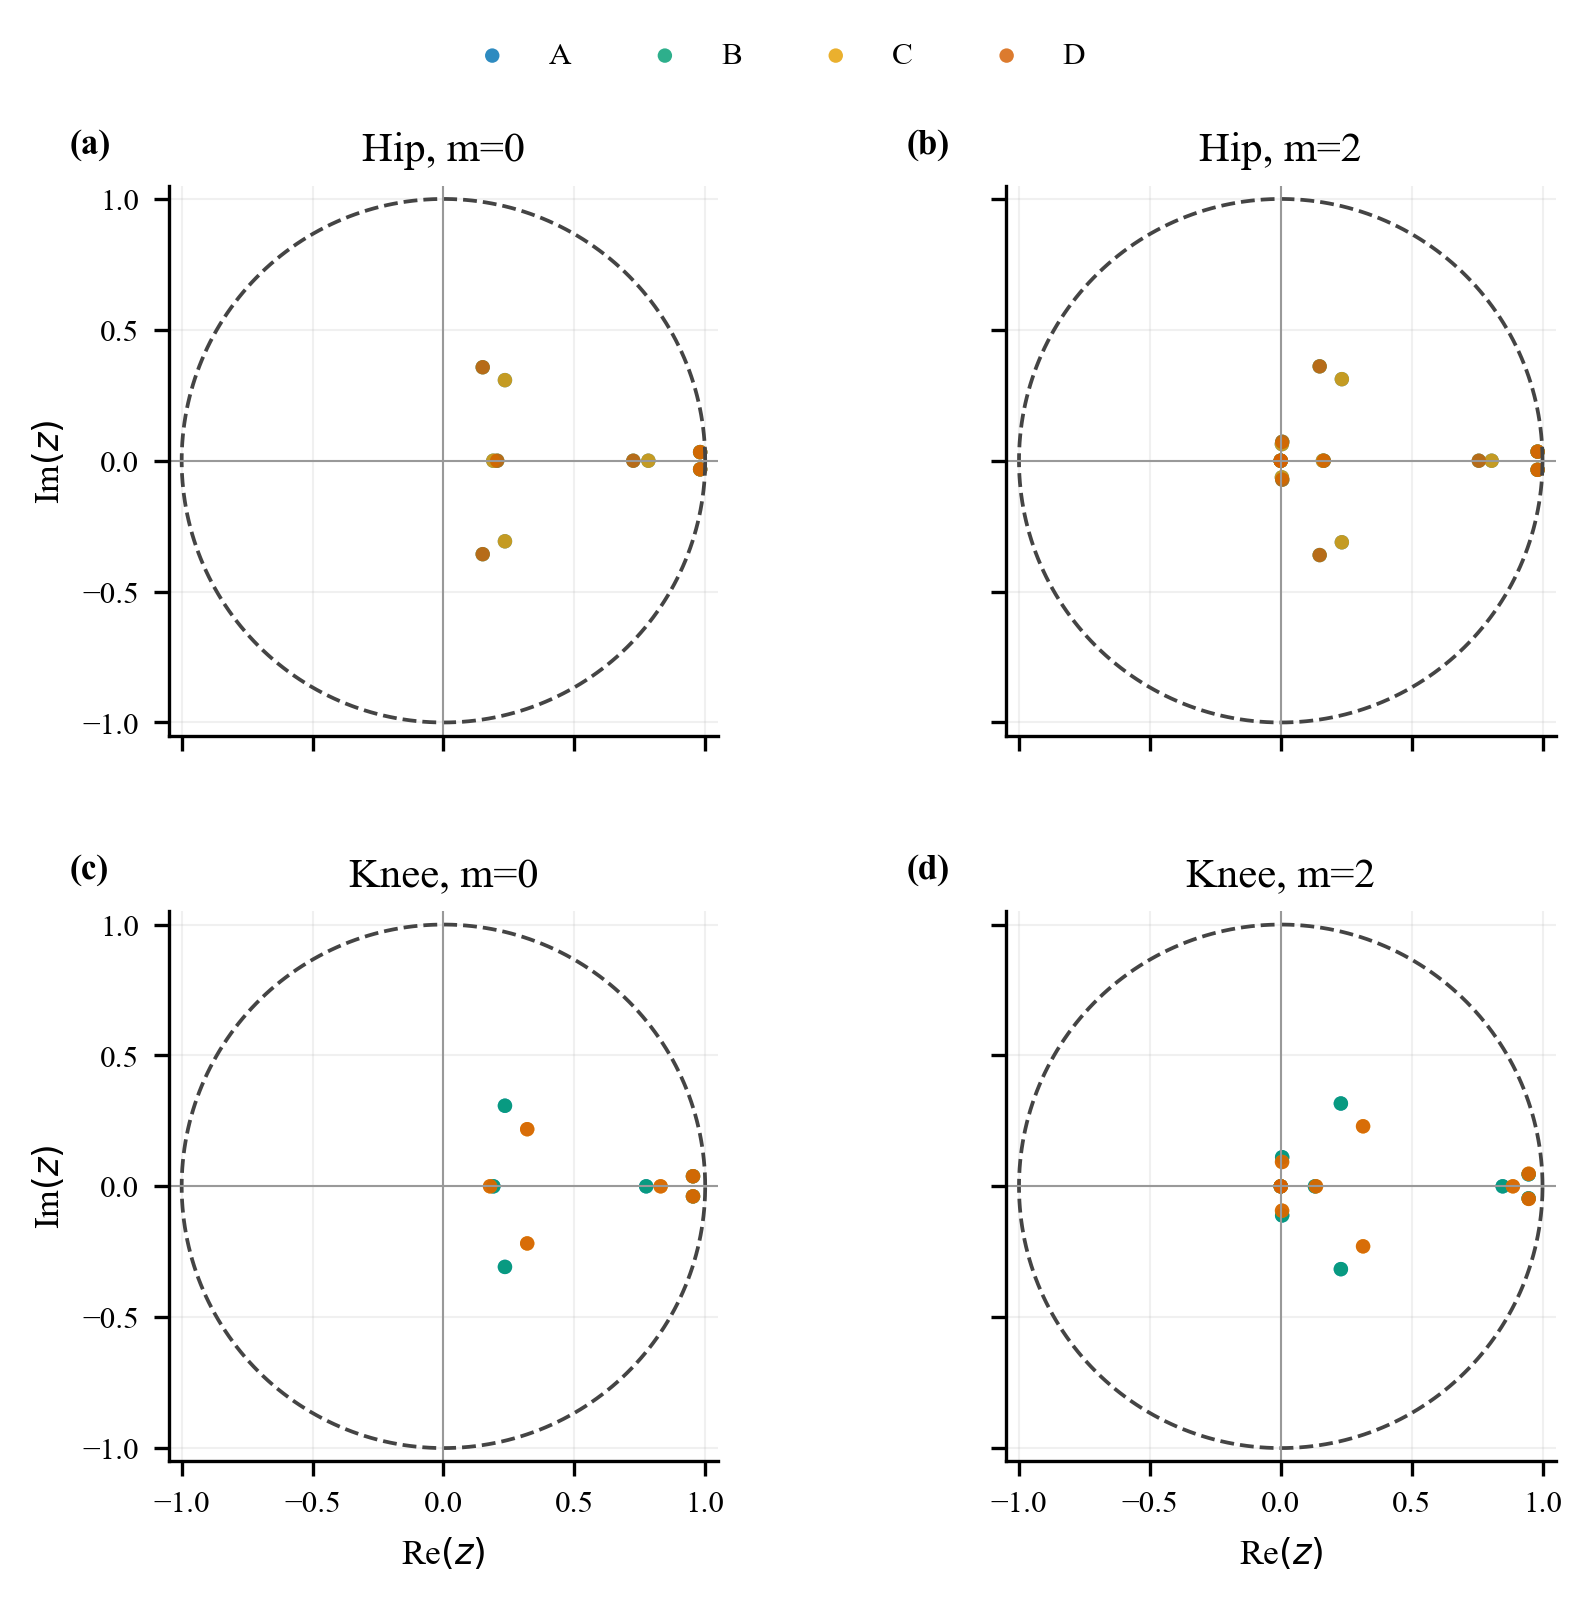
\includegraphics[keepaspectratio,alt={MuJoCo 增广闭环 z 平面极点}]{analysis_artifacts/bychen_mujoco_sweep/mujoco_deep_analysis/figures/bychen_mujoco_augmented_zplane_poles.png}}
\caption{MuJoCo 日志辨识的局部增广闭环极点。在该局部模型中未发现单位圆外极点，但该结果不能写成实机全局稳定性结论。}
\end{figure}

\begin{figure}[H]
\centering
\pandocbounded{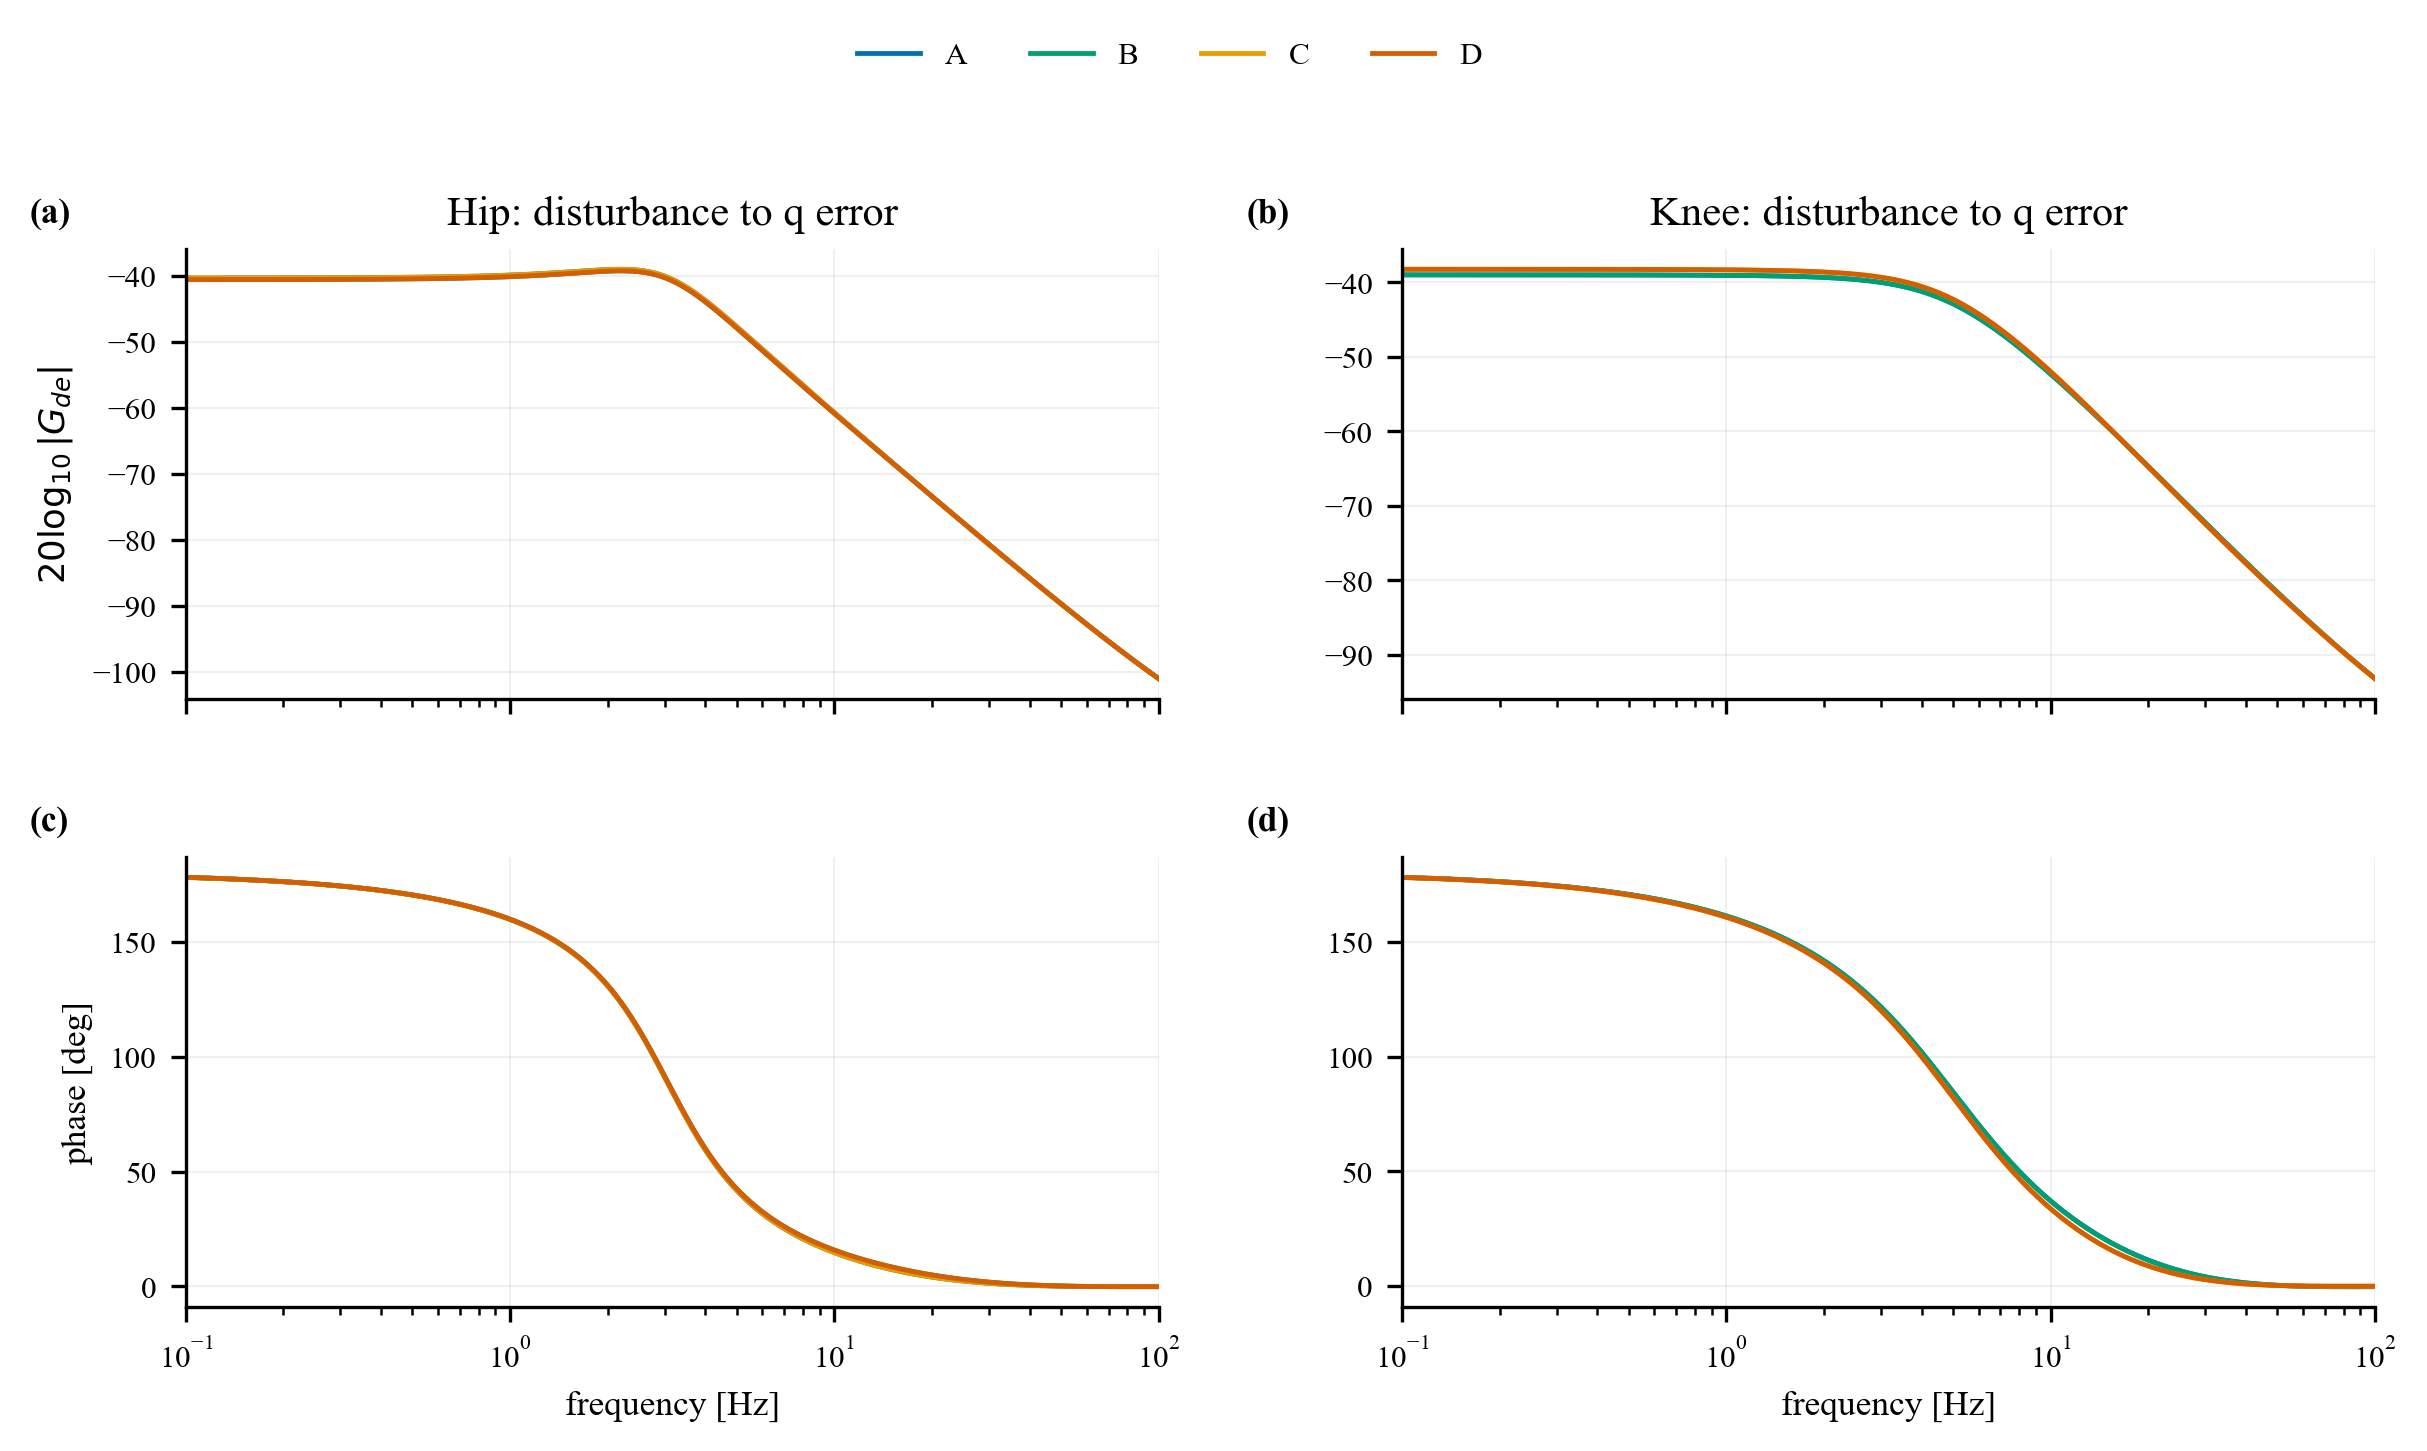
\includegraphics[keepaspectratio,alt={辨识模型扰动到误差 Bode}]{analysis_artifacts/bychen_mujoco_sweep/mujoco_deep_analysis/figures/bychen_mujoco_identified_bode_disturbance.png}}
\caption{辨识模型扰动到误差 Bode。该图用于比较候选的局部扰动抑制趋势。}
\end{figure}

\begin{figure}[H]
\centering
\pandocbounded{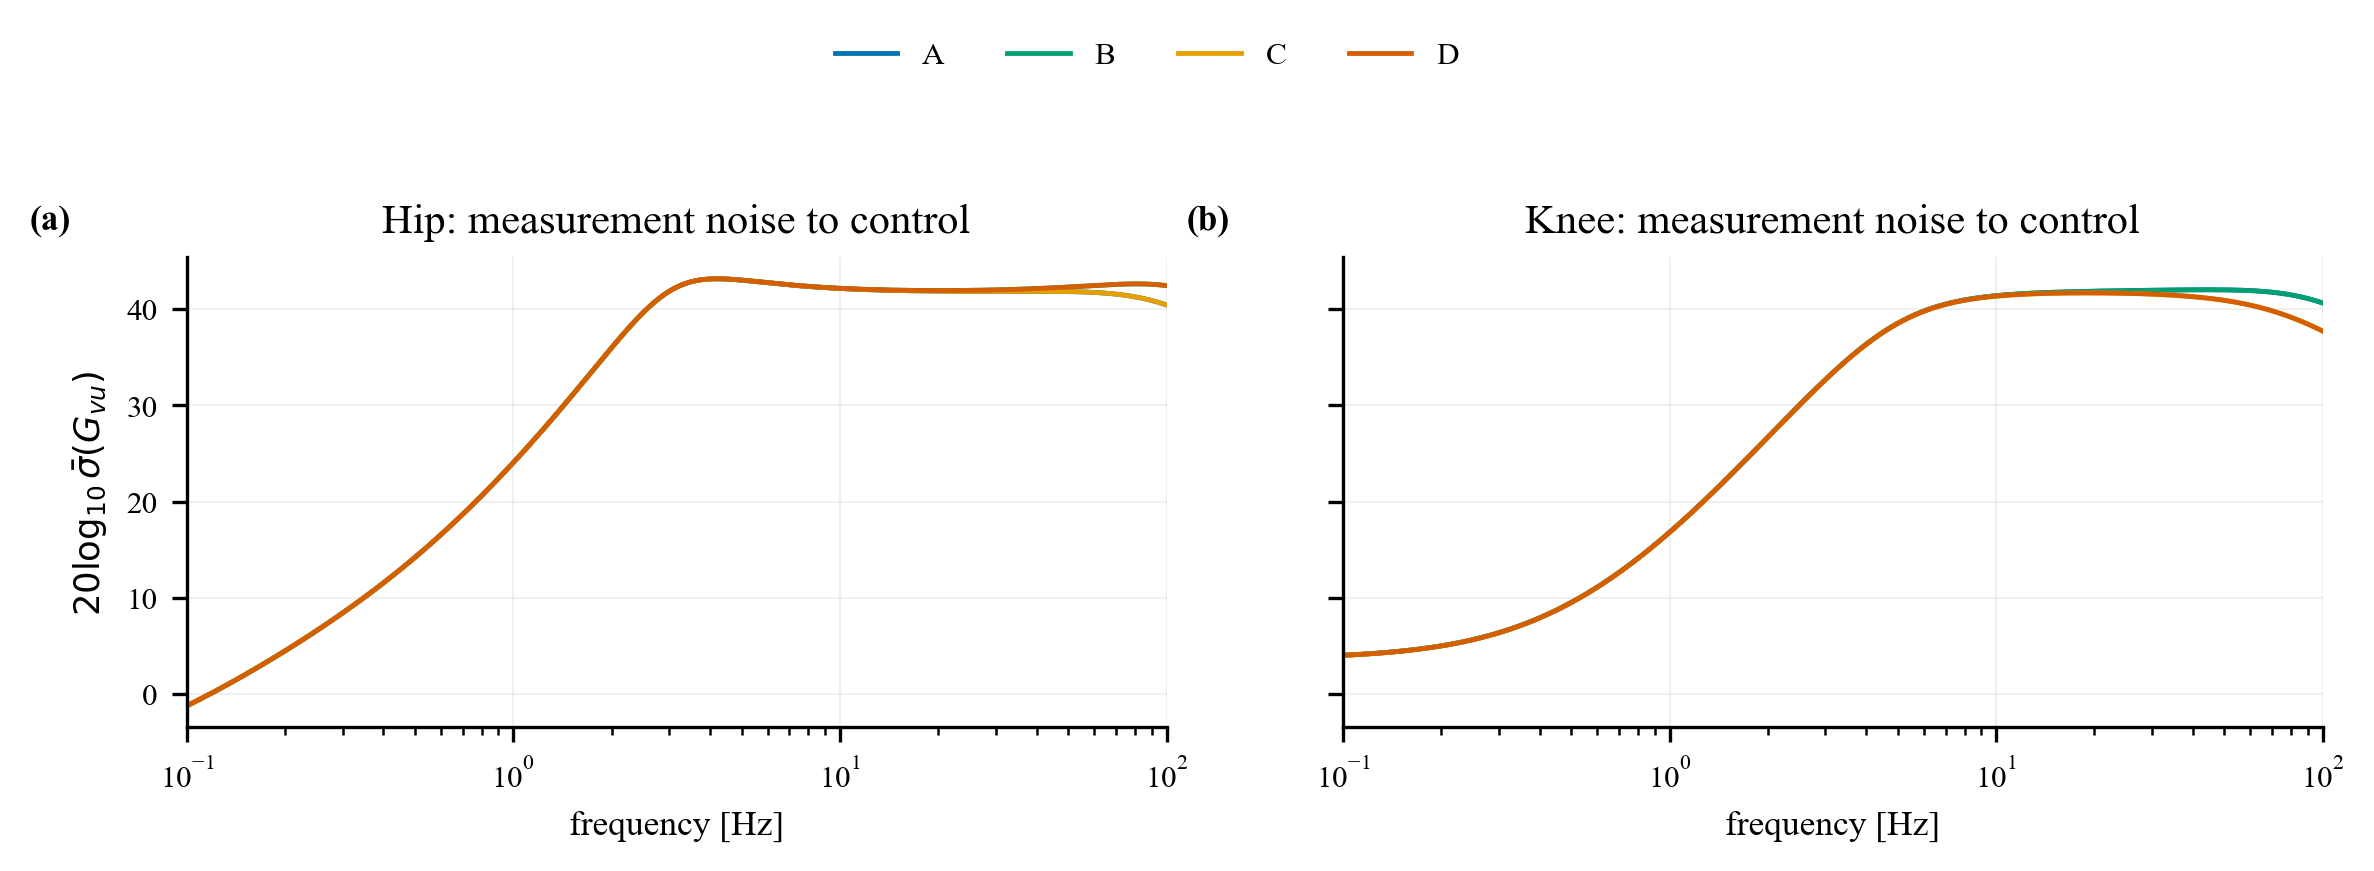
\includegraphics[keepaspectratio,alt={辨识模型测量噪声到控制奇异值}]{analysis_artifacts/bychen_mujoco_sweep/mujoco_deep_analysis/figures/bychen_mujoco_identified_noise_singular_value.png}}
\caption{辨识模型测量噪声到控制奇异值。C/D 在局部模型中略降低膝测量噪声到控制输出峰值，但不改善膝扰动到误差峰值增益。}
\end{figure}



\end{document}
